\documentclass[a4paper,11pt]{article}
\pdfoutput=1 % if your are submitting a pdflatex (i.e. if you have
             % images in pdf, png or jpg format)

\usepackage{jheppub} % for details on the use of the package, please
                     % see the JHEP-author-manua

\usepackage{graphicx,epsfig,wrapfig,amssymb,color,amsmath,bm}

\usepackage[T1]{fontenc} % if needed


%============= FORMATING (A4) ======================================
%\setlength{\textwidth}{17cm}
%\setlength{\textheight}{26.2cm}
%\setlength{\topmargin}{-1cm}
%\renewcommand{\baselinestretch}{1.5}

\bibliographystyle{JHEP}


%=================== USE COLOURS =====================================

 
\usepackage{hyperref} %links in the table of contents
\hypersetup{
    colorlinks,
    citecolor=black,
    filecolor=black,
    linkcolor=black,
    urlcolor=black
}

\newcommand{\green}[1]{{\color{green} #1}}
\newcommand{\blue}[1]{{\color{blue} #1}}
\newcommand{\red}[1]{{\color{red} #1}}

%===================  NEW COMMANDS  ==================================
\newcommand{\be}{\begin{equation}}
\newcommand{\ee}{\end{equation}}
\newcommand{\ba}{\begin{eqnarray}}
\newcommand{\ea}{\end{eqnarray}}
\newcommand{\la}{\langle}
\newcommand{\ra}{\rangle}
\newcommand{\di}{ {\rm d} }
\newcommand{\with}[3]{{\Biggl|{\renewcommand*{\arraystretch}{0.8}
	\begin{array}{l} 
	\phantom{X}\\
	\mbox{\scriptsize ${#1}$}\\
	\mbox{\scriptsize ${#2}$}\\
	\mbox{\scriptsize #3}\end{array}}}}
%
%\newcommand{\xbj}{x}                   % Bjorken variable
%\newcommand{z}{z}
%\newcommand{\de}{d}                    % integration measure
%\newcommand{\ii}{i}                    % imaginary unit
%\newcommand{\eps}{\epsilon}
%\newcommand{\Tr}{\rm Tr} % Trace operator
%\newcommand{\half}{ {\textstyle\frac{1}{2}} }
\newcommand{\slim}{\mskip 1.5mu}       % small space in math
%\newcommand{\bm}{\boldsymbol}
%\newcommand{\bm}{\boldmath}
%\newcommand{\lf}{\left}
%\newcommand{\rg}{\right}
%\newcommand{\h}{\hat{\vec{h}}}
\def\T{_{_T}}
\def\C{_{_C}}

%Editing commands
\newcommand{\TD}{{\bf TODO:}}
\newcommand{\AP}[1]{{\bf AP:} {\color{red} #1}}

\definecolor{darkgreen}{rgb}{0,0.65,0}
\newcommand{\darkgreen}[1]{{\color{darkgreen} #1}}
\newcommand{\PS}[1]{\blue{\bf\boldmath #1}}


\newcommand{\SB}[1]{{\bf SB:} {\color{magenta} #1}}
\newcommand{\judge}[1]{{\boldmath \ ({\lowercase\blue{#1}}, PS)}}



\newcommand{\asym}[2]{{A_{#1}^{#2}}}
\newcommand{\asympre}[2]{{A_{#1,\langle y\rangle}^{#2}}}





 
 % PETER'S DEFINITIONS
%\def\bfkperp{{\bf p}_T} 
%\def\bfpperp{{\bf k}_T} 
%\def\bfhp{{\bf h}_\perp} 
%\def\bfPhperp{{\bf P}_{h\perp}}
%\def\Phperp{P_{h\perp}}

%\def\kperp{p_T}
%\def\pperp{k_T}
%\def\avkperp{\la \kperp^2 \ra}
%\def\avpperp{\la \pperp^2 \ra}

\def\bflperp{{\bm \ell}_\perp} 

 % STANDARD DEFINITIONS
 %INT conventions:
\newcommand{\vect}[1]{\ensuremath{{\bm{#1}}}}
\def\bfkperp{{\bm k}_\perp} 
\def\bfpperp{{\bm P}_\perp} 
\def\bfhp{\hat{\bm h}} 
\def\bfPhperp{{\bm P}_{hT}}
\def\Phperp{P_{hT}}

\def\kperp{k_\perp}
\def\pperp{P_\perp}
\def\avkperp{\la \kperp^2 \ra}
\def\avpperp{\la \pperp^2 \ra}


\newcommand*{\FigPath}{./figs}%  
\newcommand*{\BibPath}{.}%  



%===================  TITLE, AUTHORS, AFFILIATIONS ===================

 
\preprint{JLAB-THY-17-XXXX}


\title{	Semi-Inclusive Deep Inelastic Scattering 
	in Wandzura-Wilczek-type approximation}

\author[a]{S.~Bastami}
%\author[b]{M.~D.~Albright}
\author[c]{H.~Avakian}
\author[d]{A.~V.~Efremov} 
\author[e]{A.~Kotzinian} 
\author[f]{B.~U.~Musch} 
\author[e]{B.~Parsamyan} 
\author[b,c]{A.~Prokudin} 
\author[g]{M.~Schlegel} 
\author[a,g]{P.~Schweitzer} 
\author[g]{W.~Vogelsang} 


\affiliation[a]{Department of Physics, University of Connecticut, 
	Storrs, CT 06269, U.S.A.}
\affiliation[b]{Division of Science, Penn State Berks, Reading, 
	PA 19610, USA}
\affiliation[c]{Thomas Jefferson National Accelerator Facility, 
	Newport News, VA 23606, U.S.A.}
\affiliation[d]{Joint Institute for Nuclear Research, Dubna, 
	141980 Russia}
\affiliation[e]{Dipartimento di fisica teorica, Universit\`a degli 
   studi di Torino, and Sezione dell'INFN di Torino, Via Pietro Giuria 1, 
   10125 Torino, Italy}
\affiliation[f]{Institut f\"ur Theoretische Physik, Universit\"at 
  	Regensburg, 93040 Regensburg, Germany}
\affiliation[g]{Institute for Theoretical Physics, Universit\"at T\"ubingen,
	% Auf der Morgenstelle 14, 
	D-72076 T\"ubingen, Germany}

% e-mail addresses: one for each author, in the same order as the authors
\emailAdd{saman.bastami@uconn.edu}
%\emailAdd{mda5232@psu.edu} % Mason Dale Albright
\emailAdd{avakian@jlab.org}
\emailAdd{efremov@theor.jinr.ru}
\emailAdd{aram.kotzinian@cern.ch}
\emailAdd{bmusch@b-mu.de}
\emailAdd{bakur@cern.ch}
\emailAdd{prokudin@jlab.org}
\emailAdd{marc.schlegel@uni-tuebingen.de}
\emailAdd{peter.schweitzer@phys.uconn.edu}
\emailAdd{werner.vogelsang@uni-tuebingen.de}


%\date{\today}
%===================  PREPRINT NUMBER, JOURNAL =======================
%\
%===================  ABSTRACT =======================================
%\begin{abstract}
\abstract{ 
We present the complete cross-section for pion production in Semi-Inclusive 
Deep Inelastic Scattering (SIDIS) in the Wandzura-Wilczek-type approximation 
up to power-suppressed ${\cal O}(1/Q^2)$ terms. We compute all % 18 
twist-2 and twist-3 SIDIS structure functions and the corresponding 
asymmetries. We discuss  the applicability of the
Wandzura-Wilczek-type approximations on the basis of available data,
and make predictions which can be tested by data from 
Jefferson Lab, COMPASS, HERMES, and the future EIC. 
The results of this paper can be readily used for phenomenology and 
for event generators for SIDIS, and will help to improve our 
understanding of the TMD theory beyond leading twist.
} 
%\end{abstract}
%\pacs{13.88.+e, % Polarization in interactions and scattering
%      13.85.Ni, % Inclusive production with identified hadrons
%      13.60.-r, % Photon and charged-lepton interactions with hadrons
 %     13.85.Qk} % Hadron-induced inclusive production with identified leptons, 
                % photons, or other nonhadronic particles (energy > 10 GeV)
\keywords{
	Wandzura-Wilczek approximation, 
	semi-inclusive deep inelastic scattering, 
	transverse momentum dependent distribution functions, 
	spin and azimuthal asymmetries, leading and subleading twist}

 
%%%%%%%%%%%%%%%%%%%%%%%%%%%%%%%%%%%%%%%%%%
\begin{document}
%%%%%%%%%%%%%%%%%%%%%%%%%%%%%%%%%%%%%%%%%%

\maketitle

\flushbottom

%======= SECTION 1: INTRODUCTION =====================================
\section{Introduction}
\label{Sec-1:introduction}

A great deal of what is known about the quark-gluon structure of 
nucleon is due to studies of parton distribution functions (PDFs) 
in deeply inelastic reactions. Leading-twist PDFs  tell us  how likely 
it is to find an unpolarized parton 
(described by PDF $f_1^a(x)$, $a=q,\,\bar q,\,g$) 
or a longitudinally polarized parton 
(described by PDF $g_1^a(x)$, $a=q,\,\bar q,\,g$)
in a fast-moving unpolarized or longitudinally polarized nucleon, 
which carries the fraction $x$ of the nucleon momentum.
This information depends on the ``resolution (renormalization) scale'' 
associated with the hard scale $Q$ of the process.
%, which we will not indicate for notational simplicity.
Although the PDFs  $f_1^a(x)$ and $g_1^a(x)$ continue being the 
subject of intense research (small-$x$, large-$x$, helicity sea 
and gluon distributions) they can be considered as rather 
well-known, and the frontier has been extended in the last years 
to go beyond the one-dimensional picture offered by PDFs.

One way to do this consists in a systematic inclusion of transverse 
parton momenta $\kperp$ whose effects manifest themselves in terms of
transverse momenta of the reaction products in the final state.
If these transverse momenta are much smaller than the hard scale $Q$
of the process, the formal description is given in terms of 
transverse momentum dependent distribution functions (TMDs) 
and fragmentation functions (FFs)
which are defined in terms of quark-quark correlators 
\cite{Mulders:1995dh,Boer:1997nt,Goeke:2005hb,Bacchetta:2006tn},
and depend on two independent variables: the fraction $x$ of 
nucleon momentum carried by parton, and intrinsic transverse 
momentum $\kperp$ of the parton.
Being a vector in the plane transverse with respect to the
light-cone direction singled out by the hard momentum flow in the process,
$\kperp$ allows us to access novel information on the nucleon spin structure 
through correlations of $\kperp$ with nucleon and/or parton spin. The 
latter is a well-defined concept for twist-2 TMDs interpreted in 
the infinite momentum frame or in lightcone quantization formalism.

One powerful tool to study TMDs are measurements of the SIDIS process.
By exploring various possibilities for electron/muon beam and target 
polarizations unambiguous information can be accessed on the 8 leading-twist 
TMDs \cite{Boer:1997nt} and, if one assumes factorization, on certain
linear combinations of the 16 subleading-twist TMDs 
\cite{Goeke:2005hb,Bacchetta:2006tn}.
Complementary information can be obtained 
from the Drell-Yan process \cite{Arnold:2008kf}, 
and $e^+e^-$ annihilation \cite{Metz:2016swz}.

In QCD the TMDs are independent functions. Each TMD contains unique
information on a different aspect of the nucleon structure. 
Twist-2 TMDs have partonic interpretations. Twist-3 TMDs 
give insights on quark-gluon correlations in the nucleon
\cite{Miller:2007ae,Burkardt:2007rv,Burkardt:2009rf}. 
Besides positivity constraints \cite{Bacchetta:1999kz} 
there is little model-independent information on TMDs. 
An important question with practical applications is:
do useful {\sl approximations} for TMDs exist? 
Experience from collinear PDFs encourages to explore this possibility: 
the twist-3 $g_T^a(x)$ and $h_L^a(x)$ can be expressed in terms of 
contributions from twist-2 $g_1^a(x)$ and $h_1^a(x)$, and additional 
quark-gluon-quark ($\bar{q}gq$) correlations or current quark mass 
terms \cite{Wandzura:1977qf,Jaffe:1991ra}. 
We shall refer to the latter generically as $\bar qgq$-terms, keeping in 
mind one deals in each case with matrix elements of different operators.
The $\bar qgq$-correlations contain new insights on hadron structure 
which are worthwhile exploring for their own sake, 
see \cite{Jaffe:1989xx} on $g_T^a(x)$.

The striking observation is that the $\bar qgq$-terms in $g_T^a(x)$ 
and $h_L^a(x)$ are small: theoretical mechanisms predict this 
\cite{Balla:1997hf,Dressler:1999hc,Gockeler:2000ja,Gockeler:2005vw}, 
and in the case of $g_T^a(x)$ data confirm or are compatible with these 
predictions \cite{Abe:1998wq,Anthony:2002hy}.
This approximation (``neglect of $\bar qgq$-terms'') is commonly 
known as Wandzura-Wilczek (WW) approximation \cite{Wandzura:1977qf}.
The possibility to apply this type of approximation also to TMDs has 
been explored in specific cases in \cite{Kotzinian:1995cz,Kotzinian:1997wt,
Kotzinian:2006dw,Avakian:2007mv,Metz:2008ib,Teckentrup:2009tk}.
In both cases, PDFs and TMDs, one basically assumes that the 
contributions from $\bar{q}gq$-terms can be neglected with respect to 
$\bar{q}q$-terms. But the nature of the omitted matrix elements is 
different, and in the context of TMDs one often prefers to speak 
about WW-type approximations.

In this work, after introducing the SIDIS process and defining TMDs and FFs 
(Sec.~\ref{Sec-2:SIDIS+TMDs+FF}), we shall introduce the approximations,
and review what is presently known about their reliability from experiment 
and theory (Sec.~\ref{Sec-3:WW}).
We will show that under the assumption of the validity of these approximations 
it is possible to describe all leading and subleading SIDIS structure functions
in terms of a basis of 6 TMDs and 2 FFs, and review what is presently known
about these functions (Sec.~\ref{Sec-4:SIDIS-in-WW-approximation}).
Using the latest available extractions of the 8 basis functions  
we will systematically apply the WW and/or WW-type approximations
to SIDIS structure at leading (Sec.~\ref{Sec-6:twist-2-and-WW}) 
and subleading (Sec.~\ref{Sec-7:twist-3-and-WW}) twist.
We will conclude with a critical discussion (Sec.~\ref{Sec-8:conclusions}).

This is the first study of all SIDIS structure functions up to twist-3 
in a unique approach. Our results are of use for experiments prepared 
in the near-term (Jefferson Lab 12) or proposed in the long-term 
(Electron Ion Collider), and provide helpful input for Montecarlo event
generators \cite{Avakian:2015vha}.
Our predictions will either be confirmed within the expected accuracy, 
implying the approximations work and calling for dedicated theoretical 
explanations why. Or they will fail in certain cases, calling for 
theoretical work to explain why in some cases $\bar{q}gq$-terms are sizable.
In any case, our results will deepen our understanding.

\newpage
%======= SECTION 2: SIDIS & TMDs & FFs ===============================
\section{The SIDIS process in terms of TMDs and FFs}
\label{Sec-2:SIDIS+TMDs+FF}

In this section we review the description of the SIDIS process, 
define structure functions, PDFs, TMDs, FFs and recall how they
describe the SIDIS structure functions.

\subsection{The SIDIS process}
\label{Sec-2.1:SIDIS+structure-functions}

%------ BEGIN FIGURE 1: Kinematics of SIDIS ---------------------------
\begin{wrapfigure}[8]{RD}{8cm}
\vspace{-5mm}
\centering
	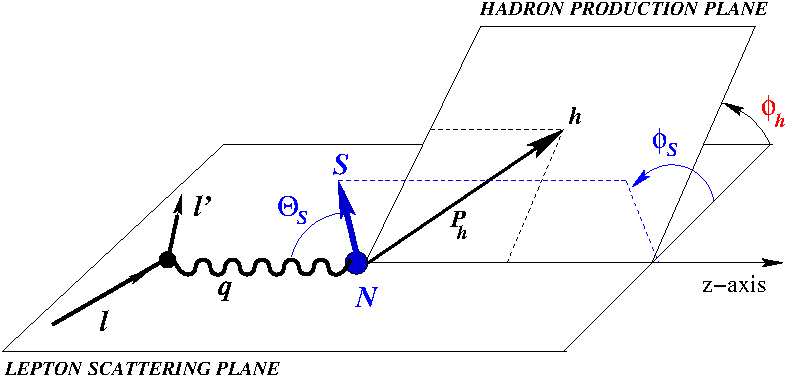
\includegraphics[width=7.5cm]{\FigPath/Fig02a-kin-SIDIS-UT.eps}
        \caption{\label{fig-kin-SIDIS}
    	Kinematics of SIDIS process $lN\to l^\prime h X$.} 
	% and the definitions of azimuthal angles in the lab frame.}
\vspace{-5mm}
\end{wrapfigure}
%------ END FIGURE 1 -------------------------------------------------

The SIDIS process is sketched in 
Fig.~\ref{fig-kin-SIDIS}. Here $l$ and $P$ are momenta of incoming 
lepton and nucleon, and $l^\prime$ and $P_h$ are the momenta of the outgoing
electron and produced hadron. The virtual photon momentum $q=l-l^\prime$ 
selects a z-axis, and $l^\prime$ points in the direction of the x-axis 
from which azimuthal angles are counted. The relevant kinematic invariants 
are
\ba
   x  = \frac{Q^2}{2\,P\cdot  q}, \;\;
   y = \frac{P \cdot  q}{P \cdot  l}, \;\;
   z = \frac{P \cdot  P_h}{P\cdot  q}, \;\;
%   \gamma = \frac{2 M x}{Q} \; .
   Q^2=-q^2.
\label{eq:xyz}\;\;\;\;\ea
In addition to $x$, $y$, $z$ the cross section is also differential 
in the azimuthal angle $\phi_h$ of the produced hadron, the square 
of its momentum component $\Phperp$ perpendicular with respect to the 
virtual photon momentum, and the azimuthal angle $\psi_l$ characterizing 
the overall orientation of the lepton scattering plane in the lab frame.
Notice that $d \psi_l \simeq d\phi_S$ where $\phi_S$ is the azimuthal angle
of the nucleon spin vector. It is convenient to define the unpolarized
lepton -- quark scattering cross section
\ba\label{Eq:sigma0-FUU}
	\sigma_0 \equiv \frac{d \sigma}{dy} 
	= 
	\frac{4 \pi \alpha_{em}^2}{x\,y\,Q^2}
	\biggl(1-y+\frac12y^2\biggr)\;
\ea


To leading order in $1/Q$ the SIDIS cross-section is given by  
\begin{subequations}\ba\hspace{-1cm}
   &&  \frac{d^6\sigma_{\rm leading}}{dx\,dy\,dz\,d\phi_S\,d\phi_h\,d \Phperp^2}
   =	 \frac{\sigma_0 }{4\pi}\; F_{UU}(x,z,\Phperp^2)
        \Biggl\{\;1 
        + \cos(2\phi_h)\,   p_1\,A_{UU}^{\cos(2\phi_h)} \nonumber\\
   && \hspace{2cm}
  	+ S_L\sin(2\phi_h)\,p_1\,A_{UL}^{\sin(2\phi_h)}    
	+ \lambda\,S_L\,    p_2\,A_{LL}  \phantom{\frac11}\nonumber\\
   && \hspace{2cm}
	+ \lambda\,S_T\cos(\phi_h-\phi_S)\,p_2\,A_{LT}^{\cos( \phi_h-\phi_S)}
       	+ S_T\sin( \phi_h-\phi_S)\, A_{UT}^{\sin( \phi_h-\phi_S)} \phantom{\frac11}
	\nonumber\\ 
   && \hspace{2cm}
	+ S_T\sin( \phi_h+\phi_S)\,p_1\,A_{UT}^{\sin( \phi_h+\phi_S)} 
        + S_T\sin(3\phi_h-\phi_S)\,p_1\,A_{UT}^{\sin(3\phi_h-\phi_S)}\Biggr\}
    \hspace{1cm} \label{Eq:SIDIS-leading}
\ea
where $F_{UU}$ is the structure function due to transverse
polarization of the virtual photon (sometimes denoted as $F_{UU,T}$),
and we systematically neglect $1/Q^2$ corrections in 
kinematic factors and a structure function arising from
longitudinal polarization of the virtual photon 
(sometimes denoted as $F_{UU,L}$). %  poorly known in SIDIS.
The structure functions (and asymmetries $A$) also depend on $Q^2$ via the scale dependence of 
TMDs and FFs, which we do not show in formulas throughout this work.

At subleading order one has
\ba\hspace{-1cm}
   &&   \frac{d^6\sigma_{\rm subleading}}{dx\,dy\,dz\,d\phi_S\,d\phi_h\,d \Phperp^2}
   =	\frac{\sigma_0 }{4\pi} \; F_{UU}(x,z,\Phperp^2)
        \Biggl\{ 
          \cos(\phi_h)\,p_3\,A_{UU}^{\cos(\phi_h)}
  	{}
	\nonumber\\ 
   && \hspace{2cm}
	+ \lambda\sin(\phi_h)\,p_4\,A_{LU}^{\sin(\phi_h)}+ S_L\sin(\phi_h)\,p_3\,A_{UL}^{\sin(\phi_h)}    
	+ S_T\sin(\phi_S)\,p_3\,A_{UT}^{\sin(\phi_S)} \phantom{\frac11}\nonumber\\ 
   && \hspace{2cm}
	+ S_T\sin(2\phi_h-\phi_S)\,p_3\,A_{UT}^{\sin(2\phi_h-\phi_S)}
        + \lambda\,S_L\cos(\phi_h)\,p_4\,A_{LL}^{\cos(\phi_h)}\phantom{\frac11}
	\nonumber\\
   && \hspace{2cm}
  	+ \lambda\,S_T\cos(\phi_S)\,p_4\,A_{LT}^{\cos(\phi_S)}
        + \lambda\,S_T\cos(2\phi_h-\phi_S)\,p_4\,A_{LT}^{\cos(2\phi_h-\phi_S)}
	\Biggr\}
   \hspace{1cm} \label{Eq:SIDIS-subleading}
\ea\end{subequations}
Neglecting $1/Q^2$ corrections, the kinematic prefactors $p_i$ are given by 
% \ba\label{Eq:y-prefactors}
% &&	p_1 = \varepsilon \equiv  
%        \frac{1-y -\frac{1}{4}\slim \gamma^2 y^2}{1-y
%        + \frac{1}{2}\slim y^2 +\frac{1}{4}\slim \gamma^2 y^2} 
%        \approx \frac{1-y}{1-y+\frac12\,y^2} 		\;,\nonumber\\
% &&	p_2 = \sqrt{1-\epsilon^2} \approx
%        \frac{y(1-\frac12\,y)}{1-y+\frac12\,y^2} 	\;,\nonumber\\
% &&	p_3 =  \sqrt{2\varepsilon(1+\varepsilon)}
%        \approx \frac{(2-y)\sqrt{1-y}}{1-y+\frac12\,y^2}\;,\nonumber\\
% &&	p_4 =  \sqrt{2\varepsilon(1-\varepsilon)}
%        \approx \frac{y\sqrt{1-y}}{1-y+\frac12\,y^2} 	\;,\;\;\;
% \ea
\be\label{Eq:y-prefactors}
	p_1 = \frac{1-y}{1-y+\frac12\,y^2} 		\, , \;\;\;
	p_2 = \frac{y(1-\frac12\,y)}{1-y+\frac12\,y^2}	\, , \;\;\;
	p_3 = \frac{(2-y)\sqrt{1-y}}{1-y+\frac12\,y^2} 	\, , \;\;\;
	p_4 = \frac{y\sqrt{1-y}}{1-y+\frac12\,y^2}     	\, .
\ee
and the asymmetries are defined as 
\be
	A_{XY}^{\rm weight}\equiv A_{XY}^{\rm weight}(x,z,\Phperp)=
	\frac{F_{XY}^{\rm weight}(x,z,\Phperp)}{F_{UU}(x,z,\Phperp)}.
\ee
Hereby the first index $X=U(L)$ denotes the unpolarized beam
(longitudinally polarized beam with helicity $\lambda$).
The second index $Y=U(L,T)$ refers to the target which can be unpolarized
(or longitudinally, transversely polarized with respect to virtual photon).
The superscript ``weight'' indicates the azimuthal dependence with no index 
indicating an isotropic angular distribution of the produced hadrons.

Experimental collaborations often define asymmetries in terms of counts 
$N(\phi_h)$. This means the kinematic prefactors $p_i$ and $1/(x\,y\,Q^2)$ 
are included in the numerators or denominators of the asymmetries which
are averaged over $y$ within experimental kinematics. We will call the 
corresponding asymmetries $\asympre{XY}{\rm weight}$.
For instance, in unpolarized case one has 
\be
	N(\phi) = \frac{N_0}{2\pi} \biggl(1
		+ \cos\phi\;\asympre{UU}{\cos\phi_h}+
		+ \cos2\phi\;\asympre{UU}{\cos2\phi_h}\Biggr)
\ee
where $N_0$ denotes the total $\phi_h$-averaged)\
number of counts in the kinematic bin of interest.
It would be preferable if asymmetries were analyzed with known kinematic 
prefactors divided out on event-by-event basis. One could then directly 
compare asymmetries $\asym{XY}{\rm weight}$ measured in different 
experiments and kinematics, and focus on effects of evolution 
or power suppression for twist-3. In practice, data analysis is easier
with kinematic factors included. Data for such asymmetries 
$\asympre{XY}{\rm weight}$ are more easily available. We will 
define and comment on the explicit expressions as needed.

For completeness we remark that after integrating the cross section
over transverse hadron momenta one obtains 
\begin{subequations}\ba
     	\frac{d^4\sigma_{\rm leading}}{dx\,dy\,dz\,d\phi_S}
   &=&	 \frac{\sigma_0 }{2\pi}\; F_{UU}(x,z) 
        \Biggl\{\;1 + \lambda\,S_L\,    p_2\,A_{LL} \Biggr\}
    	\label{Eq:SIDIS-leading-integrated} \\
	\frac{d^4\sigma_{\rm subleading}}{dx\,dy\,dz\,d\phi_S}
   &=&	 \frac{\sigma_0 }{2\pi}\; F_{UU}(x,z) 
        \Biggl\{ S_T\sin(\phi_S)\,p_3\,A_{UT}^{\sin(\phi_S)} 
  	+ \lambda\,S_T\cos(\phi_S)\,p_4\,A_{LT}^{\cos(\phi_S)}
          \Biggr\}
     \hspace{1cm} \label{Eq:SIDIS-subleading-integrated}
\ea\end{subequations}
where (and analog for the other structure functions)
\be\label{Eq:FUU-integrated}
	F_{UU}(x,z) = \int d^2\Phperp\;F_{UU}(x,z,\Phperp)
\ee
and the asymmetries are defined as
\be
	A_{XY}^{\rm weight}(x,z) = \frac{F_{XY}^{\rm weight}(x,z)}{F_{UU}(x,z)}\,.
\ee

The connection of ``collinear'' SIDIS structure functions
in (\ref{Eq:SIDIS-leading-integrated},~\ref{Eq:SIDIS-subleading-integrated})
to those known from inclusive DIS is established by integrating over $z$
and summing over hadrons as 
\begin{subequations}\begin{alignat}{4}
	&\sum\limits_h\int d z\;z\;F_{UU}(x,z) 
	&\equiv	&&	& 2\,x\,F_1(x) \;, 
	\label{Eq:DIS-F1}\\ % x\sum_q e_q^2\,f_1^q(x) 
	&\sum\limits_h\int d z\;z\;F_{LL}(x,z) 
	&\equiv && 	& 2\,x\,g_1(x) \;, 
	\label{Eq:DIS-g1}\\ % x\sum_q e_q^2\,g_1^q(x) 
	&\sum\limits_h\int d z\;z\;F_{LT}^{\cos\phi_S}(x,z) \;\;
	&\equiv && \;\; -\,\gamma\; & 2\,x\biggl(g_1(x)+g_2(x)\biggr) \;, 
	\label{Eq:DIS-gT}\\ % -\,\frac{2M_Nx^2}{Q} \sum_q e_q^2\,g_T^q(x) 
	&\sum\limits_h\int d z\;z\;F_{UT}^{\sin\phi_S}(x,z) 
	&=      && 	    & \;\; 0 \, ,
	\label{Eq:DIS-zero}
\end{alignat}\end{subequations}
where $\gamma=2M_Nx/Q$ signals the twist-3 character of $F_{LT}^{\cos\phi_S}(x,z)$.
We consequently neglect $1/Q^2$ effects, including the twist-4 DIS structure 
function $F_2(x)$. $F_{UT}^{\sin\phi_S}(x,z)$ has no DIS counterpart due to 
time reversal symmetry of strong interactions. 

\subsection{TMDs, FFs and structure functions}
\label{Sec-2.2:def-TMD-FF}

TMDs are defined in terms of light-front correlators
\be\label{Eq:correlator}
    	\Phi(x,\bfkperp)_{ij} = \int\frac{ d \xi^- d^2{\bm \xi}_\perp}{(2\pi)^3}
	\;e^{ik\xi}\;\la N(P,S)|\bar\psi_j(0)\,{\cal W}_{(0,\,\infty)}
	{\cal W}_{(\infty,\xi)}\,\psi_i(\xi)|N(P,S)\ra
    	\with{ }{\xi^+\!=\!0}{$k^+ = xP^+$}
	\ee
where the symbolic Wilson-lines refer to the SIDIS process 
\cite{Collins:2002kn}. For a generic four-vector $a^\mu$ we define
the light-cone coordinates $a^\mu=(a^+,a^-,a_\perp)$ with 
$a^\pm=(a^0\pm a^3)/\sqrt{2}$. 
The light-cone direction is singled out by the virtual photon momentum 
and transverse vectors like $\bfkperp$ are perpendicular to it. In the
virtual-photon--nucleon center-of-mass frame, nucleon and the partons 
inside it move in the $(+)$-lightcone direction, while the struck 
quark and the produced hadron move in $(-)$-light-cone direction.
In the nucleon rest frame the polarization vector is given by 
$S=(0,{\bm S}_T,S_L)$ with ${\bm S}_T^2+S_L^2=1$.


\newpage

The 8 leading-twist TMDs \cite{Boer:1997nt} are projected out from the
correlator (\ref{Eq:correlator}) as follows
(\blue{blue (online only): T-even}, \red{red  (online only): T-odd}; we suppress flavor
and renormalization scale dependence)
\begin{subequations}\ba
    \frac12\;{\rm Tr}\biggl[\gamma^+ \;\Phi(x,\bfkperp)\biggr]
    &=& \hspace{5mm}
    \blue{f_1}-\frac{\varepsilon^{jk}\kperp^j S_T^k}{M_N}\,\red{f_{1T}^\perp}\;, 
    \label{Eq:TMD-pdfs-I}\\
    \frac12\;{\rm Tr}\biggl[\gamma^+\gamma_5 \;\Phi(x,\bfkperp)\biggr] &=&
    S_L\,\blue{g_1} + \frac{\bfkperp \cdot{\bm S}_T}{M_N}\,\blue{g_{1T}^\perp}\;, 
    \label{Eq:TMD-pdfs-II}\\
    \frac12\;{\rm Tr}\biggl[i\sigma^{j+}\gamma_5 \;\Phi(x,\bfkperp)\biggr] &=&
    S_T^j\,\blue{h_1}  + S_L\,\frac{\kperp^j}{M_N}\,\blue{h_{1L}^\perp} +
    \frac{\kappa^{jk}S_T^k}{M_N^2}\,
    \blue{h_{1T}^\perp} + \frac{\varepsilon^{jk}\kperp^k}{M_N}\,\red{h_1^\perp}\;, 
    \label{Eq:TMD-pdfs-III} \hspace{15mm}
\ea
and the 16 subleading twist TMDs \cite{Mulders:1995dh,Bacchetta:2006tn}
are given by
\ba
\hspace{-5mm}    
	\frac12{\rm Tr}\biggl[\,1\;\Phi(x,\bfkperp)\biggr]         &=&
    	\frac{M_N}{P^+}\biggl[
	\hspace{5mm}\blue{e}
	-\frac{\varepsilon^{jk}\kperp^j S_T^k}{M_N}\,\red{e_T^\perp}
    	\biggr], \label{Eq:sub-TMD-pdfs-I}\\
\hspace{-5mm}    
	\frac12{\rm Tr}\biggl[i\gamma_5\Phi(x,\bfkperp)\biggr]        &=&
        \frac{M_N}{P^+}\biggl[
    	S_L\red{e_L} +\frac{\bfkperp \cdot {\bm S}_T}{M_N}\,\red{e_T}
    	\biggr], \label{Eq:sub-TMD-pdfs-II}\\
\hspace{-5mm}    
	\frac12{\rm Tr}\biggl[\,\gamma^j\,\Phi(x,\bfkperp)\biggr]        &=&
        \frac{M_N}{P^+}\biggl[
    	\frac{\kperp^j}{M_N}\blue{f^\perp}\!+\varepsilon^{jk}S_T^k\red{f_T}
	\!+\!S_L\frac{\varepsilon^{jk}\kperp^k}{M_N}\red{f_L^\perp}
	\!-\!\frac{\kappa^{jk}\varepsilon^{kl}S_T^l}{M_N^2}\red{f_T^\perp}\!
	\biggr], \label{Eq:sub-TMD-pdfs-III}\\
\hspace{-5mm}    
	\frac12{\rm Tr}\biggl[\,\gamma^j\gamma_5\Phi(x,\bfkperp)\biggr] &=&
    	\frac{M_N}{P^+}\biggl[
    	S_T^j\,\blue{g_T} 
	+ S_L\,\frac{\kperp^j}{M_N}\blue{g_L^\perp} +
	\frac{\kappa^{jk}S_T^k}{M_N^2}
    	\,\blue{g_T^\perp} 
	+\frac{\varepsilon^{jk}\kperp^k}{M_N}\,\red{g^\perp} 
	\biggr], \label{Eq:sub-TMD-pdfs-IV}\\
\hspace{-5mm}    
	\frac12{\rm Tr}\biggl[i\,\sigma^{jk}\gamma_5\Phi(x,\bfkperp)\biggr] &=&
    	\frac{M_N}{P^+}\biggl[
    	\frac{S_T^j \kperp^k-S_T^k \kperp^j}{M_N}\,\blue{h_T^\perp}
    	-\varepsilon^{jk}\,\red{h} 
	\biggr], \label{Eq:TMD-pdfs-V} \\
\hspace{-5mm}    
	\frac12{\rm Tr}\biggl[i\,\sigma^{+-}\,\gamma_5\,\Phi(x,\bfkperp)\biggr] 
	&=& \frac{M_N}{P^+}\biggl[
    	S_L\,\blue{h_L} + \frac{\bfkperp\cdot{\bm S}_T}{M_N}\,\blue{h_T}
    	\biggr]. \label{Eq:TMD-pdfs-VI}
\ea\end{subequations}
where $\kappa^{jk}\equiv (\kperp^j \kperp^k-\frac12\,\bfkperp^{\:2}\delta^{jk})$.
The indices $j,k,l$ refer to the plane transverse with respect to the
light-cone, $\epsilon^{ij}\equiv\epsilon^{-+ij}$ and $\epsilon^{0123}=+1$.
Dirac-structures not listed in (\ref{Eq:TMD-pdfs-I}--\ref{Eq:TMD-pdfs-VI}) 
are twist-4 \cite{Goeke:2005hb}.
Integrating out transverse momenta in the correlator (\ref{Eq:correlator})
leads to the `usual' PDFs known from collinear kinematics
\cite{Ralston:1979ys,Jaffe:1991ra}, namely at twist-2 level
\begin{subequations}\ba
    \frac12\;{\rm Tr}\biggl[\gamma^+ \;\Phi(x)\biggr]
    &=& \hspace{5mm}
    \blue{f_1}\;, 	\label{Eq:pdf-I}\\
    \frac12\;{\rm Tr}\biggl[\gamma^+\gamma_5 \;\Phi(x)\biggr] &=&
    S_L\,\blue{g_1}\;, 	\label{Eq:pdf-II}\\
    \frac12\;{\rm Tr}\biggl[i\sigma^{j+}\gamma_5 \;\Phi(x)\biggr] &=&
    S_T^j\,\blue{h_1}\;, \label{Eq:pdf-III} \hspace{75mm}
\ea
and at twist-3 level
\ba
    \frac12\;{\rm Tr}\biggl[\,1\;\Phi(x)\biggr] &=&
    \frac{M_N}{P^+}\;\blue{e}\;,  \label{Eq:sub-pdf-I}\\
    \frac12\;{\rm Tr}\biggl[\gamma^j\gamma_5 \;\Phi(x)\biggr] &=&
    \frac{M_N}{P^+}\;S_T^j\,\blue{g_T} \;, \label{Eq:sub-pdf-II}\\ \hspace{6mm}
    \frac12\;{\rm Tr}\biggl[\,i\,\sigma^{+-}\gamma_5 \;\Phi(x)\biggr] 
    &=& \frac{M_N}{P^+}\;S_L\,\blue{h_L}\,. \label{Eq:sub-pdf-III}\hspace{75mm}
\ea\end{subequations}
Other structures drop out either due to explicit $\kperp$-dependence,
or due to the sum rules \cite{Bacchetta:2006tn}
\be\label{Eq:sum-rules-T-odd}
	\int d^2\bfkperp\;f_T^a(x,\kperp^2)=
	\int d^2\bfkperp\;e_L^a(x,\kperp^2)=
	\int d^2\bfkperp\;h^a(x,\kperp^2)=0
\ee
imposed by time reversal constraints.

The fragmentation functions are similarly defined in terms of the correlator
\be\label{Eq:correlator-FF}
    \Delta(z,\bfpperp)_{ij} 
    = \sum\limits_X\!\int\!
    \frac{ d \xi^+ d^2 {\bm \xi}_\perp}{2z(2\pi)^3}\,e^{ip\xi}
    \, \la 0  |{\cal W}_{(\infty,\xi)}\psi_i(\xi)\,|h,X\ra\,
    \la h,X|\bar{\psi}_j(0){\cal W}_{(0,\infty)}|0\ra
    \with{\xi^-\!=\!0}
	 {p^- \!=\! P_h^-/z}
	 {${\bm p}_\perp \!=\! -\bfpperp/z$.}
    \ee
In this work we will consider only unpolarized final state hadrons.
If the produced hadron moves fast in the $(-)$ light cone direction, 
the twist-2 FFs are projected out as 
\begin{subequations}\ba
	\frac{1}{2}{\rm Tr}\big[\gamma^-\Delta(z,\bfpperp)\big]
	&=& \blue{D_1}\, , \label{eq:DeltaTr-twist-2a}\\
	\frac{1}{2}{\rm Tr}\big[i\sigma^{j-}\gamma_5\Delta(z,\bfpperp)\big]
	&=& \epsilon^{jk}\,\frac{\pperp^k}{zm_h}\red{H_1^\perp}\;, 
	\label{eq:DeltaTr-twist-2b}
\ea
and at twist-3 level
\ba
    \frac12\;{\rm Tr}\biggl[\,1\;\Delta(z,\bfpperp)\biggr]         &=&
    \phantom{-}\frac{M_h}{P^-_h}\;\blue{E}\;,  \label{eq:DeltaTr-twist-3a}\\
    \frac12\;{\rm Tr}\biggl[\;\,\gamma^j\;\Delta(z,\bfpperp)\biggr]  &=&
    -\frac{\pperp^j}{zP_h^-}\;\blue{D^\perp}\;, \label{eq:DeltaTr-twist-3b}\\
    \frac12\;{\rm Tr}\biggl[\gamma^j\gamma_5 \,\Delta(z,\bfpperp)\biggr] &=&
    \varepsilon^{jk}\,\frac{\pperp^k}{zP_h^-}\,\red{G^\perp}\;,  
	\label{eq:DeltaTr-twist-3c}\\
    \frac12\;{\rm Tr}\biggl[i\,\sigma^{jk}\gamma_5\,\Delta(z,\bfpperp)
	\biggr] &=&
    -\varepsilon^{jk}\,\frac{M_h}{P_h^-}\;\red{H}\;.  \label{eq:DeltaTr-twist-3d}
\ea\end{subequations}
Here besides scale and flavor dependence we also do not indicate
the type of hadron $h$. Integration over transverse hadron momenta leaves
us with $D_1(z)$, $E(z)$, $H(z)$ while the other structures drop out due to 
their $\pperp$ dependence.

%\subsection{Structure functions}

The structure functions in 
Eqs.~(\ref{Eq:SIDIS-leading},~\ref{Eq:SIDIS-subleading}) are described 
in Bjorken limit at tree level in terms of convolutions of TMDs 
and FFs. We define the unit vector $\bfhp   = \bfPhperp/\Phperp$ 
and use the following convolution integrals 
(see Appendix \ref{ApendixB1} for details) 
\be
 \label{Eq:def-convolution-integral}
 {\cal C}\biggl[\omega\;f\;D\biggr]
	= x \sum_a e_a^2\int d^2\bfkperp^{ } d^2\bfpperp
 	\; \delta^{(2)}(z \bfkperp^{ }+ \bfpperp^{ }-\bfPhperp^{ })\;\omega
	%\left(\bfkperp,-\frac{\bfpperp}{z}\right)
  	\; f^a(x,\bfkperp^2)\ D^a(z,\bfpperp^2)\;,
\ee
where $\omega$ is a weight function which in general depends on 
$\bfkperp$ and $\bfpperp$.
The 8 leading-twist structure functions are 
\begin{subequations}
\label{Eqs:structure-functions-twist-2}
\ba
 F_{UU}	&=&{\cal C}\biggl[\;\omega^{\{0\}}\,f_1 D_1 \;\biggr] \label{FUU}\\
 F_{LL}	&=&{\cal C}\biggl[\;\omega^{\{0\}}\,g_1 D_1 \;\biggr] \label{FLL}\\
 F_{UT}^{\sin\left(\phi_h +\phi_S\right)} 
	&=& {\cal C}\biggl[\;\omega^{\{1\}}_{\rm A} \,h_{1} H_1^{\perp}\;\biggr]
	\label{Eq:FUTCol}\\
 F_{UT}^{\sin\left(\phi_h -\phi_S\right)} 
	&=& {\cal C}\biggl[-\,\omega^{\{1\}}_{\rm B} \,f_{1T}^{\perp } D_1\,\biggr]
	\label{Eq:FUTSiv}\\
 F_{LT}^{\cos(\phi_h -\phi_S)} 
	&=& {\cal C}\biggl[\,\omega^{\{1\}}_{\rm B} \,g_{1T}^\perp D_1\biggr] 
	\label{Eq:FLT-twist-2}\\
 F_{UU}^{\cos 2\phi_h} 	
	&=& {\cal C}\biggl[\;\omega^{\{2\}}_{\rm AB}\,h_{1}^{\perp }\,H_{1}^{\perp }\;
	\biggr] \label{F_UUcos2phi}\\
 F_{UL}^{\sin 2\phi_h} 	
	&=& {\cal C}\biggl[\;\omega^{\{2\}}_{\rm AB}\,h_{1L}^{\perp } H_{1}^{\perp }\; 
	\biggr] \label{F_UUsin2phi}\\
 F_{UT}^{\sin\left(3\phi_h -\phi_S\right)} 
	&=& {\cal C}\biggl[\;\omega^{\{3\}}_{\rm { }}\,h_{1T}^{\perp } H_1^{\perp }\; 
	\biggr] \, . \hspace{75mm} \label{Eq:FUTpretzel}
\ea\end{subequations}
At subleading-twist we have the structure functions
\begin{subequations}
\label{Eqs:structure-functions-twist-3}
\ba
	F_{UU}^{\cos\phi_h}  
	&=& 
	\frac{2M}{Q}\,{\cal C}\biggl[\phantom{-}
   	\omega^{\{1\}}_{\rm A} 
	\biggl( x h\,H_{1}^{\perp } 
   	+ r_h^{ }\,\,f_1 \frac{\tilde{D}^{\perp }}{z}\biggr)
	- \omega^{\{1\}}_{\rm B} \biggl( x  f^{\perp } D_1
   	+ r_h^{ }\,\,h_{1}^{\perp } \frac{\tilde{H}}{z}\biggr)\biggr]\;
	\label{Eq:FUUcosphi}\\
	F_{LU}^{\sin\phi_h}  
	&=& 
	\frac{2M}{Q}\,{\cal C}\biggl[ \phantom{-}
	\omega^{\{1\}}_{\rm A}
   	\biggl( x \, e \, H_1^{\perp } 
   	+ r_h^{ }\,\,f_1\frac{\tilde{G}^{\perp }}{z}\,\biggr)
   	+\omega^{\{1\}}_{\rm B}
   	\biggl( x   g^{\perp }  D_1 
   	+ r_h^{ }\,\, h_1^{\perp } \,\frac{\tilde{E}}{z} \biggr)\biggr]\;
	\label{FLUsinphi}\\
	F_{UL}^{\sin\phi_h} 
 	&=& 
	\frac{2M}{Q}\,{\cal C}\biggl[\phantom{-}
   	\omega^{\{1\}}_{\rm A}
    	\biggl( x   h_L  H_1^{\perp } \! 
   	+ r_h^{ }\,\,g_{1}\frac{\tilde{G}^{\perp } }{z}\biggr)
   	+\omega^{\{1\}}_{\rm B}
    	\biggl( x  f_{L}^{\perp }  D_1 \!
   	- r_h^{ }\,\, h_{1L}^{\perp }  \frac{\tilde{H}}{z}\biggr)\biggr]\;
	\label{FULsinphi}\\
	F_{LL}^{\cos \phi_h} 
 	&=& 
	\frac{2M}{Q}\,{\cal C}\biggl[ 
	-\omega^{\{1\}}_{\rm A}
   	\biggl( x  e_L  H_1^{\perp }
   	- r_h^{ }\,\,g_{1}   \frac{\tilde{D}^{\perp }}{z}\biggr)
   	-\omega^{\{1\}}_{\rm B}
   	\biggl( x   g_L^{\perp }   D_1
   	+  r_h^{ }\,\,h_{1L}^{\perp } \frac{\tilde{E}}{z}\biggr)\biggr]
	\label{FLLcosphi}\;\;\;\;\\
	F_{UT}^{\sin \phi_S } 
	&=&  
	\frac{2M}{Q}\,{\cal C}\biggl[ \phantom{-}
	\omega^{\{0\}}\,\biggl(x   f_T   D_1 \;
   	- r_h^{ }\, \; h_{1} \, \frac{\tilde{H}}{z} \biggr)\nonumber\\
   	&&\hspace{1.2cm}
   	-\frac{\omega^{\{2\}}_{\rm B}}{2}
	\biggl( x   h_{T}  H_{1}^{\perp } 
   	+ r_h^{ }\, g_{1T}^\perp \,\frac{\tilde{G}^{\perp }}{z}
   	- x   h_{T}^{\perp }  H_{1}^{\perp } 
	+ r_h^{ }\, f_{1T}^{\perp } \,\frac{\tilde{D}^{\perp }}{z}
   	\biggr) \biggr]\; \label{FUTsinphiS}\\ 
	F_{LT}^{\cos \phi_S} 
	&=& 
	\frac{2M}{Q}\,{\cal C}\biggl[
   	- \omega^{\{0\}}\,\biggl(x   g_T   D_1
   	+ r_h^{ }\, \, h_{1}  \frac{\tilde{E}}{z} \biggr)\nonumber\\
   	&&\hspace{1.2cm}
	+\frac{\omega^{\{2\}}_{\rm B}}{2}
   	\biggl( x   e_{T}  H_{1}^{\perp } 
   	- r_h^{ }\, g_{1T}^\perp \,\frac{\tilde{D}^{\perp }}{z}
   	+  x   e_{T}^{\perp }  H_{1}^{\perp } 
   	+ r_h^{ }\,f_{1T}^{\perp }\,\frac{\tilde{G}^{\perp }}{z}\biggr)\biggr]
	\; \label{FLTcosphiS} \\ \hspace{-5mm}
	F_{UT}^{\sin(2\phi_h -\phi_S)} 
	&=& 
	\frac{2M}{Q}\,{\cal C}\biggl[\phantom{-}
   	\frac{\omega^{\{2\}}_{\rm AB}}{2}\,
   	\biggl( x   h_{T}  H_{1}^{\perp } 
   	+ r_h^{ }\, g_{1T}^\perp \,\frac{\tilde{G}^{\perp }}{z}
        + x   h_{T}^{\perp }  H_{1}^{\perp } 
   	- r_h^{ }\, f_{1T}^{\perp } \,\frac{\tilde{D}^{\perp }}{z}
	\biggr)\nonumber\\
	&&\hspace{1.3cm}
	+
   	\omega^{\{2\}}_{\rm C}
   	\biggl( x   f_T^{\perp } D_1
   	- r_h^{ }\, \, h_{1T}^{\perp }  \frac{\tilde{H}}{z}\biggr) \biggr]
\ea
\ba
	F_{LT}^{\cos(2\phi_h - \phi_S)} 
	&=& \frac{2M}{Q}\,{\cal C}\biggl[
   	- \frac{\omega^{\{2\}}_{\rm AB}}{2}
   	\biggl( x   e_{T}  H_{1}^{\perp } 
   	- r_h^{ }\, g_{1T}^\perp \,\frac{\tilde{D}^{\perp }}{z}
	- x   e_{T}^{\perp }  H_{1}^{\perp } 
   	- r_h^{ }\, f_{1T}^{\perp } \,\frac{\tilde{G}^{\perp }}{z}\biggr)\nonumber\\
	&&\hspace{1.3cm}
   	- \omega^{\{2\}}_{\rm C}
   	\biggl( x   g_T^{\perp }   D_1
   	+ r_h^{ }\, \, h_{1T}^{\perp }  \frac{\tilde{E}}{z}\biggr)\biggr]\; 
	\label{FLTsin(2phi-phiS)}
\ea\end{subequations}
where $r_h = m_h/M_N$ and 
$F_{XY}^{\rm weight}\equiv F_{XY}^{\rm weight}(x,z,\Phperp)$.
The weight functions are defined as
\ba
&& \omega^{\{0\}}  	= 1 \, , \nonumber\\
&& \omega^{\{1\}}_{\rm A} 	= \frac{\bfhp\cdot\bfpperp^{ }}{z m_h}  \, , \;\;\;
   \omega^{\{1\}}_{\rm B} 	= \frac{\bfhp\cdot\bfkperp^{ }}{M_N}\,,\nonumber\\
&& \omega^{\{2\}}_{\rm A} 	=  \frac{2\, \bigl(\bfhp\cdot\bfpperp^{ }\bigr)\,
			\bigl(\bfhp\cdot\bfkperp^{ }\bigr)}{zM_Nm_h}\,,\;\;\;
   \omega^{\{2\}}_{\rm B}	= -\frac{\bfpperp^{ }\cdot\bfkperp^{ }}{zM_Nm_h}\,,\;\;\;
   \omega^{\{2\}}_{\rm C}	= \frac{2\,(\bfhp\cdot\bfkperp^{ })^2-\bfkperp^2}{2M_N^2}
			\, ,\nonumber\\
&& \omega^{\{3\}}_{\rm{ }}	= \frac{
			 4\,(\bfhp\cdot\bfpperp^{ })\,(\bfhp\cdot\bfkperp^{ })^2
			-2\,\bigl(\bfhp\cdot\bfkperp^{ }\bigr)\, 
        		\bigl(\bfkperp^{ }\cdot\bfpperp^{ }\bigr)
   			-\bigl(\bfhp\cdot\bfpperp^{ }\bigr)\,\bfkperp^2\
   			}{2 z M_N^2 m_h}\,,
			\label{Eq:wi} \ea
and $\omega^{\{2\}}_{\rm AB} = \omega^{\{2\}}_{\rm A} + \omega^{\{2\}}_{\rm B}$.
In $\omega^{\{n\}}_{i}$ the index $n=0,\,1,\,2,\,3$ indicates the (maximal)
power $(\Phperp)^N$ with which the corresponding contribution scales,
and index $i$ (if any) distinguishes different types of contributions
at the given order $N$.
Notice that twist-3 structure functions in 
Eqs.~(\ref{Eq:FUUcosphi}--\ref{FLTsin(2phi-phiS)}) contain an explicit 
factor $M/Q$. We also recall that we neglect two structure functions 
due to longitudinal virtual photon polarization which contribute,
in the TMD factorization framework, at order ${\cal O}(M^2/Q^2)$, 
one being $F_{UU,L}$ and the other contributing to the 
$\sin(\phi_h-\phi_S)$ angular distribution \cite{Bacchetta:2006tn}.

The structures surviving $\Phperp$-integration of the SIDIS cross section in 
(\ref{Eq:SIDIS-leading-integrated},~\ref{Eq:SIDIS-subleading-integrated})
are associated with the trivial weights $\omega^{\{0\}}$ and expressed in 
terms of collinear PDFs and FFs as follows (here the 
sum rules (\ref{Eq:sum-rules-T-odd}) are used)
\begin{subequations}\ba
	F_{UU}(x,z) &=& x\sum\limits_ae_a^2\,f_1^a(x)\,D_1^a(z)
	\label{Eq:FUU-collinear}\\
	F_{LL}(x,z) &=& x\sum\limits_ae_a^2\,g_1^a(x)\,D_1^a(z)
	\label{Eq:FLL-collinear}\\
 	F_{LT}^{\cos\phi_S}(x,z) &=& -\,\frac{2M_N}{Q}\; x\sum_a e_a^2\,
	\biggl(x\,g_T^q(x) + r_h\,h_1^a(x)\frac{\tilde{E}^a(z)}{z}\biggr)
	\label{Eq:FLT-collinear}\\
	 F_{UT}^{\sin\phi_S}(x,z) &=& -\,\frac{2\,m_h}{Q}\; x\sum_a e_a^2\,
	h_1^a(x)\frac{\tilde{H}^a(z)}{z}
	\label{Eq:FUT-collinear}
\ea\end{subequations}
Finally, using the sum rules for the T-odd FFs 
$\sum_h\int d z\;\tilde{E}^a(z)=0$ and
$\sum_h\int d z\;\tilde{H}^a(z)=0$ we recover
Eqs.~(\ref{Eq:DIS-F1}--\ref{Eq:DIS-zero}) and obtain for the DIS structure 
functions
\begin{subequations}\ba
    F_1(x) & = & \frac{1}{2}\sum_a e_a^2\,f_1^a(x) \label{Eq:DIS-F1-II}\\
    g_1(x) & = & \frac{1}{2}\sum_a e_a^2\,g_1^a(x) \label{Eq:DIS-g1-II}\\
    g_2(x) & = & \frac{1}{2}\sum_a e_a^2\,g_T^a(x)\;-\;g_1(x) \label{Eq:DIS-g2}
	\hspace{25mm}
\ea\end{subequations}
Having established the notation we now define and discuss the
approximations. 


%======= SECTION 3: WW APPROXIMATIONS ================================
\section{WW and WW-type approximations}
\label{Sec-3:WW}

In this section we will define the approximations and review what is
known about them.
The basic idea of the approximations is simple. One assumes that the 
contributions from $\bar{q}gq$-terms can be neglected with respect to 
$\bar{q}q$-terms with a useful accuracy,
\be\label{Eq:WW-generic}
	\biggl|\frac{\la\bar{q}gq\ra}{\la\bar{q}q\ra}\biggr| \ll 1\,.
\ee

\subsection{WW approximation for PDF\lowercase{s}}
\label{Sec-3.1:WW-classic}

The WW approximation applies in principle to all twist-3 PDFs,
Eqs.~(\ref{Eq:sub-pdf-I},~\ref{Eq:sub-pdf-II},~\ref{Eq:sub-pdf-III}).
It was established first for $g_T^a(x)$ \cite{Wandzura:1977qf}, and 
later for $h_L^a(x)$ \cite{Jaffe:1991ra}. The situation of $e^a(x)$ 
is somewhat special, see below and the review \cite{Efremov:2002qh}.

The origin of the approximations is as follows.
The operators defining $g_T^a(x)$ and~$h_L^a(x)$ can be decomposed by means 
of QCD equations of motion in twist-2 parts, and pure twist-3 
(interaction dependent) $\bar qgq$-terms and current quark mass
terms. We denote $\bar qgq$-terms and mass-terms collectively 
and symbolically by functions with a tilde.
Such decompositions are possible because $g_T^a(x)$ and $h_L^a(x)$ are 
``twist-3'' not according to the ``strict QCD definition''
(twist $=$ mass dimension of associated local operator minus its spin).
Rather they are classified according to the ``working definition'' 
\cite{Jaffe:1996zw}  
(a function is ``twist $t$'' if it contributes to cross sections
suppressed by $(M/Q)^{t-2}$ with $M$ a generic hadronic and $Q$ the 
hard scale).
The two definitions coincide for twist-2 quantities, but higher twist
observables in general contain ``contaminations'' by leading twist.

In this way one obtains the decompositions and, if they apply, WW 
approximations \cite{Wandzura:1977qf,Jaffe:1991ra} (keep in mind 
here tilde terms contain pure twist-3 and current quark mass terms)
\begin{subequations}\begin{alignat}{3}
   	g_T^a(x) &=& 
        \phantom{2x}\;\int_x^1\frac{ d y}{y}\,g_1^a(y) + &\tilde{g}_T^a(x)
        \stackrel{\rm WW}{\approx} 
        \phantom{2x}\;\int_x^1\frac{ d y}{y}\,g_1^a(y) \;, 
	\label{Eq:WW-original1} \\
   	h_L^a(x) &=& 2x\int_x^1\frac{ d y}{y^2}\,h_1^a(y) + &\tilde{h}_L^a(x)
        \stackrel{\rm WW}{\approx} 2x\int_x^1\frac{ d y}{y^2}\,h_1^a(y)\;,
	\label{Eq:WW-original2}\\
   	x\,e^a(x) &=& x\,&\tilde{e}^a(x) \;\stackrel{\rm WW}{\approx} 
	\;\;\;\; 0
\end{alignat}\end{subequations}
where we included $e^a(x)$ which ia a special case in the sense that it 
receives no twist-2 contribution. Notice that a prefactor of $x$ is
provided to cancel a $\delta(x)$-type singularity \cite{Efremov:2002qh}.
After introducing the WW-type approximations for TMDs and FFs,
we will come back to (\ref{Eq:WW-original1},~\ref{Eq:WW-original2}) and 
review the theoretical predictions and experimental data supporting them.

\subsection{WW-type approximations for TMDs and FFs}
\label{Sec-3.2:WW-type-TMD-FF}

Analog to WW approximations for PDFs discussed in 
Sec.~\ref{Sec-3.1:WW-classic}, also certain TMDs and FFs
can be decomposed in twist-2 contributions and tilde-terms.
The latter may be assumed, in the spirit of (\ref{Eq:WW-generic}),
to be small. Hereby it is important to keep in mind that one deals 
with different types of (``unintegrated'') $\bar qgq$-correlations,
and we prefer to refer to them as WW-type approximations.

In the T-even case one obtains the following approximations,
where the terms on the left-hand-side are twist-3, those on the 
right-hand-side (if any) are twist-2,
\begin{subequations}\ba
xe^q(x,\kperp^2)	&\stackrel{\rm WW-type}{\approx}& 
			0, 
			\label{Eq:WW-type-1}\\
xf^{\perp q}(x,\kperp^2)  &\stackrel{\rm WW-type}{\approx}& 
			f_{1}^q(x,\kperp^2),
			\label{Eq:WW-type-Cahn}\phantom{\frac11}\\
xg_L^{\perp q}(x,\kperp^2)&\stackrel{\rm WW-type}{\approx}& 
			g_{1}^q(x,\kperp^2),
			\label{Eq:WW-type-gLperp}\phantom{\frac11}\\
xg_T^{\perp q}(x,\kperp^2)&\stackrel{\rm WW-type}{\approx}& 
			g_{1T}^{\perp q}(x,\kperp^2),\phantom{\frac11}
			\label{Eq:WW-type-gTperp}\\
xg_T^q(x,\kperp^2)   	&\stackrel{\rm WW-type}{\approx}& 
             		g_{1T}^{\perp(1)q}(x,\kperp^2), 
			\label{Eq:WW-type-5}\\
xh_L^q(x,\kperp^2)	&\stackrel{\rm WW-type}{\approx}& -2 \,
                       	h_{1L}^{\perp(1)q}(x,\kperp^2),\phantom{\frac11}
                       	\label{Eq:WW-type-6}\\
xh_T^q(x,\kperp^2)      &\stackrel{\rm WW-type}{\approx}& 
                       	- h_1^q(x,\kperp^2) - h_{1T}^{\perp(1)}(x,\kperp^2),
                       	\label{Eq:WW-type-7}\\
xh_T^{\perp q}(x,\kperp^2)&\stackrel{\rm WW-type}{\approx}& 
                       	\phantom{-}h_1^q(x,\kperp^2)-h_{1T}^{\perp(1)}(x,\kperp^2).
                       	\phantom{\frac11} \label{Eq:WW-type-8}
\ea\end{subequations}
In the T-odd case one obtains the approximations
\begin{subequations}\ba
xe_L^q(x,\kperp^2)         	&\stackrel{\rm WW-type}{\approx}& 0, \\
xe_T^q(x,\kperp^2)         	&\stackrel{\rm WW-type}{\approx}& 0, \\
xe_T^{\perp q}(x,\kperp^2) 	&\stackrel{\rm WW-type}{\approx}& 0, \\
xg^{\perp q}(x,\kperp^2)   	&\stackrel{\rm WW-type}{\approx}& 0, 
                       	\label{Eq:WW-type-gperp}\\
xf_L^{\perp q}(x,\kperp^2) 	&\stackrel{\rm WW-type}{\approx}& 0, 
			\phantom{\frac11}\\
xf_T^{\perp q}(x,\kperp^2) 	&\stackrel{\rm WW-type}{\approx}& 
                       	\phantom{-}\,f_{1T}^{\perp q}(x,\kperp^2),
			\phantom{\frac11}
                       	\label{Eq:WW-type-fTperp}\\
xf_T^{q}(x,\kperp^2)       	&\stackrel{\rm WW-type}{\approx}& 
                       	-\,f_{1T}^{\perp(1)q}(x,\kperp^2), \label{Eq:WW-type-fT}\\
xh^q(x,\kperp^2)           	&\stackrel{\rm WW-type}{\approx}& 
                       	- 2\,{h_1^{\perp(1)}(x,\kperp^2)},\phantom{\frac11 XXXXx} 
                       	\label{Eq:WW-type-last} 
\ea\end{subequations}
where the superscript ``(1)'' denotes transverse 
moments of TMDs defined generically as  
\ba
f^{(1)}(x,\kperp^2) = \frac{\kperp^2}{2M^2}\,f(x, \kperp^2)\; , \;\;\;
f^{(1)}(x ) = \int d^2 \bfkperp f^{(1)}(x,\kperp^2) \; . 
\ea 

Two very useful WW-type approximations follow from combining the
WW approximations (\ref{Eq:WW-original1},~\ref{Eq:WW-original2}) with the
WW-type approximations (\ref{Eq:WW-type-5},~\ref{Eq:WW-type-6}).
This yields \cite{Tangerman:1994bb,Mulders:1995dh,Avakian:2007mv}
\begin{subequations}\ba
   	g_{1T}^{\perp(1)a}(x)&\stackrel{\rm WW-type}{\approx}& 
        \phantom{-} x\,\int_x^1\frac{d y}{y\;}\,g_1^a(y) \;,
	\label{Eq:WW-approx-g1T}\\
    	h_{1L}^{\perp(1)a}(x)&\stackrel{\rm WW-type}{\approx}& -
	x^2\!\int_x^1\frac{d y}{y^2\;}\,h_1^a(y)\;.
	\label{Eq:WW-approx-h1L}
\ea\end{subequations}
Aspects and phenomenological applications of some of the above
WW-type approximations were discussed in 
\cite{Tangerman:1994bb,Kotzinian:1995cz,Mulders:1995dh,Kotzinian:1997wt,
Kotzinian:2006dw,Avakian:2007mv,Metz:2008ib,Teckentrup:2009tk}.

WW-relations for FFs are actually not needed: in Eqs.~%
(\ref{Eqs:structure-functions-twist-2},~\ref{Eqs:structure-functions-twist-2})
either twist-2 FFs $D_1^a$, $H_1^{\perp a}$ enter or tilde FFs, as a consequence 
of how the azimuthal angles are defined \cite{Bacchetta:2006tn}. 
For completeness we quote the WW-type approximations for FFs
\cite{Bacchetta:2006tn}
\begin{subequations}\ba
	E(z,\pperp^2)      &\stackrel{\rm WW-type}{\approx}& 0 \, ,
	\label{Eq:WW-type-FF-1}\\
	G^\perp(z,\pperp^2) &\stackrel{\rm WW-type}{\approx}& 0 \, ,
	\label{Eq:WW-type-FF-2}\\
	D^\perp(z,\pperp^2) &\stackrel{\rm WW-type}{\approx}
	& \hspace{11mm}z\,D_1(z,\pperp^2)\,, \label{Eq:WW-type-FF-3}\\
	H(z,\pperp^2) &\stackrel{\rm WW-type}{\approx}& 
	-\frac{\pperp^2}{zM_h^2}\;H_1^\perp(z,\pperp^2)\,. \label{Eq:WW-type-FF-4}
\ea\end{subequations}
Having introduced the WW- and WW-type approximations, we will review
in the following what is currently known from theory and experiment 
about our approximations.

\subsection{Predictions from instanton vacuum model}
\label{Sec-3.3:WW-classic-instanton}

Insights on the relatve size of hadronic matrix elements, such as 
Eq.~(\ref{Eq:WW-generic}), require a non-perturbative approach. It is 
by no means obvious which small parameter in the strong interaction 
regime would allow to explain such results.

A powerful non-perturbative approach is provided by the instanton model 
of the QCD vacuum \cite{Shuryak:1981ff,Diakonov:1983hh,Diakonov:1995qy}.
This semi-classical approach assumes that properties of the QCD vacuum 
are dominated by instantons and anti-instantons, topological non-perturbative 
gluon field configurations, which form a strongly interacting medium.
The approach provides a natural mechanism for dynamical chiral symmetry 
breaking, the dominant feature of strong interactions in the nonperturbative
regime. It was shown with variational and numerical methods that the strongly
interacting instanton medium is dilute. The ratio of average instanton size 
$\rho_{\rm av}$ and average instanton separation $R_{\rm av}$ is a non-trivial
small parameter, numerically $\rho_{\rm av}/R_{\rm av}\sim1/3$ 
\cite{Shuryak:1981ff,Diakonov:1983hh,Diakonov:1995qy}, 
which can be explored.

Applying the instanton vacuum model to studies of $g_T^a(x)$ and $h_L^a(x)$
it was predicted that matrix elements of the $\bar qgq$ operators defining 
$\tilde{g}_T^a(x)$ \cite{Balla:1997hf} and $\tilde{h}_L^a(x)$ 
\cite{Dressler:1999hc} are strongly suppressed by powers of the small
parameter $\rho_{\rm av}/R_{\rm av}$ with respect to contributions from the 
respective twist-2 parts which are of the order $(\rho_{\rm av}/R_{\rm av})^0$. 
Numerically it was found 
\be\label{Eq:WW-instanoton}
	\biggl|\frac{\la\bar{q}gq\ra}{\la\bar{q}q\ra}\biggr| \sim 
	\biggl(\frac{\rho}{R}\biggr)^{\!4} \log\biggl(\frac{\rho}{R}\biggr)
	\sim 10^{-2}
\ee
in these 2 cases. This result strongly supports the generic approximation
in Eq.~(\ref{Eq:WW-generic}) with the instanton packing fraction providing 
the non-trivial small parameter justifying the neglect of tilde-terms. 
The instanton calculus has not yet been applied to $\tilde{e}^a(x)$.

Noteworthy, the instanton vacuum predictions for $\tilde{g}_T^a(x)$
were made before the advent of the first precise data on $g_2(x)$
which we discuss in the next section.

\newpage
\subsection{Tests of WW approximation in DIS experiments}
\label{Sec-3.4:WW-classic-experiment}

The presently available phenomenological information on $g_T^a(x)$ is due 
to measurements of the structure function $g_2(x)$, Eq.~(\ref{Eq:DIS-g2}),
in DIS off various transversely polarized targets. In the WW-approximation 
(\ref{Eq:WW-original1}) one can write $g_2(x)$ as a total derivative
expressed in terms of the experimentally well known twist-2
structure function $g_1(x)$ as follows
\be
    	g_2(x) \stackrel{\rm WW}{\approx} g_2(x)_{\rm WW} \equiv
	\frac{ d\;}{ d x}\;\Biggl[\frac{x}{2}\int_x^1\frac{ d y}{y}
	\;g_1(y)\Biggr]\,.\label{Eq:g2-in-WW-approximation}
\ee
Data support (\ref{Eq:g2-in-WW-approximation}) to a good accuracy
\cite{Anthony:2002hy,Abe:1998wq}, although especially at smaller 
$x$ more stringent tests are not yet possible. Overall it has been
estimated that the WW approximation for $g_2(x)$ and $g_T^a(x)$ works 
with an accuracy of about $40\,\%$ or better \cite{Accardi:2009au}. 

%%%%%%%%%%%%%%%%%%%%%%%%%%%%%%%%%%%%%%%%%%%%%%%%%%%%%%%%%%%%%%%%%%%%%%%%%%%%%%%
\begin{figure}[t!]
\centering
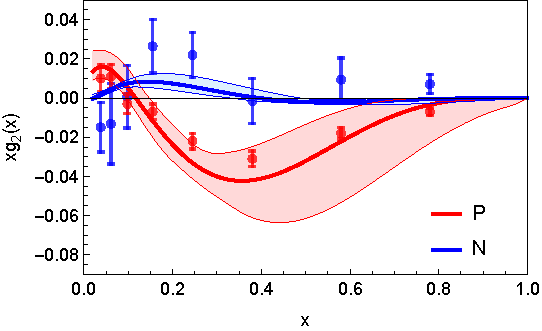
\includegraphics[width=0.6\textwidth]{\FigPath/g2.pdf} 
\caption{\label{Fig:g2} 
$g_{2}$ structure function in  WW-approximation, 
Eq.~(\ref{Eq:g2-in-WW-approximation}), for proton (P) and neutron (N)
targets. The data are from \cite{Anthony:2002hy,Abe:1998wq}.
The error band procedure is described in the text.}
\end{figure}
%%%%%%%%%%%%%%%%%%%%%%%%%%%%%%%%%%%%%%%%%%%%%%%%%%%%%%%%%%%%%%%%%%%%%%%%%%%%%%%

We present calculations of $g_2(x)_{WW}$ in Fig.~\ref{Fig:g2}.
How well does the WW approximation describe data if we allow for a
theoretical ``error band'' of about $40\,\%$ as deduced in 
\cite{Accardi:2009au}? In order to investigate this question, 
we split this uncertainty in two parts, $\varepsilon_1=\pm 20\,\%$ and 
$\varepsilon_2(x)=\pm 20\,\%(1-x)^\epsilon$ with a small $\epsilon>0$,
and estimate the impact of this uncertainty as 
\be\label{Eq:g2-in-WW-model-violation}
    g_2(x)_{\rm WW} = (1\pm\varepsilon_1)\frac{ d\;}{ d x}\;\Biggl[
    x\int_x^1\frac{ d y}{y} \,\biggl(
    \frac12\sum_ae_a^2\,g_1^a(y(1\pm\varepsilon_2))\biggr)\Biggr]\,.
\ee
The effect of $\varepsilon_1$ is to change the magnitude
of $g_2(x)_{\rm WW}$, $\varepsilon_2$ varies the position of its zero.
The $x$-dependence of $\varepsilon_2$ preserves $\lim_{x\to1}g_2(x)= 0$; 
we use $\epsilon=0.05$ which yields $\varepsilon_2\approx 20\,\%$ up to 
the highest measured $x$-bin.
The good agreement of $g_2(x)_{\rm WW}$ with data is encouraging,
and in line with theory predictions \cite{Balla:1997hf}.
Our estimate with the splitted uncertainties 
$\varepsilon_{1,2}$ may overestimate in certain $x$-bins the 
$40\,\%$-``error band'' estimated in \cite{Accardi:2009au}. This however 
helps us to display a conservative estimate of possible uncertainties.

Presently $h_L^a(x)$ is unknown.
With phenomenological information on $h_1^a(x)$
\cite{Efremov:2006qm,Anselmino:2007fs,Anselmino:2008jk}, 
the WW approximation (\ref{Eq:WW-original2}) for $h_L^a(x)$ could 
be tested experimentally in Drell-Yan \cite{Koike:2008du}.


\subsection{Tests in lattice QCD}
\label{Sec-3.5:WW-lattice}

\blue{The lowest Mellin moments of the PDF $g_T^q(x)$ were studied in
lattice QCD in the quenched approximation \cite{Gockeler:2000ja} 
and with $N_f = 2$ flavors of light dynamical quarks \cite{Gockeler:2005vw}.
The obtained results were compatible with a small $\tilde{g}_T^q(x)$. 
We are not aware of lattice QCD studies related to the PDF $h_L^a(x)$,
and turn now our attention to TMD studies in lattice QCD.

After first exploratory investigations of TMDs on the lattice
\cite{Hagler:2009mb,Musch:2010ka}, recent years have witnessed considerable
progress and} improvements with regard to rigor, realism and methodology
\cite{Yoon:2016dyh,%Proceedings of Science LATTICE 2015 (2016) 116, 
Engelhardt:2015xja,%Phys.Rev. D93 (2016) no.5, 054501, 
Ji:2014hxa,%Phys.Rev. D91 (2015) 074009, 
Musch:2011er%Phys.Rev. D85 (2012) 094510
}.
However, numerical results from recent calculations are only available 
for a subset of observables, and the quantities calculated are not in a 
form that lends itself to straighforward tests of the WW-type relations 
as presented in this paper. Details about recent works and future 
perspectives are discussed at the end of this section.

For the time being, we content ourselves with rather crude comparisons 
based on the data published in Refs.~\cite{Hagler:2009mb,Musch:2010ka}. 
These early works explored all nucleon and quark polarizations, but 
they used a gauge link that does not incorporate the final or initial 
state interactions present in SIDIS or Drell-Yan experiments. In other 
words, the transverse momentum dependent quantities computed in
\cite{Hagler:2009mb,Musch:2010ka} are not precisely the TMDs measurable 
in experiment. More caveats will be discussed along the way.

Let us now translate the approximations
(\ref{Eq:WW-approx-g1T},~\ref{Eq:WW-approx-h1L}) into expressions
for which we have a chance to compare them with available lattice data.
For that we multiply the
Eqs.~(\ref{Eq:WW-approx-g1T},~\ref{Eq:WW-approx-h1L}) by $x^N$
with $N=0,\,1,\,2,\,\dots$ and integrate over $x\in[-1,1]$ which yields
\ba
        \int_{-1}^1 d x\;x^N
       g_{1T}^{\perp(1)q}(x)&\stackrel{\rm WW-type}{\approx}&
        \phantom{-} \,\frac{1}{N+2} \int_{-1}^1 d x \;x^{N+1}g_1^q(x)
        \;,
    \label{Eq:WW-approx-g1T-d}\\
        \int_{-1}^1 d x\;x^N
        h_{1L}^{\perp(1)q}(x)&\stackrel{\rm WW-type}{\approx}&
        -\,\frac{1}{N+3} \int_{-1}^1 d x\: x^{N+1}\,h_1^q(x)
        \;.
    \label{Eq:WW-approx-h1L-d}
\ea
with the understanding that
negative $x$ refer to antiquark distributions
$g_1^{\bar q}(x) = +\,g_1^{q}(-x)$,
$h_1^{\bar q}(x) = -\,h_1^{q}(-x)$,
$g_{1T}^{\perp(1)\bar q}(x) =- g_{1T}^{\perp(1)q}(-x)$,
$h_{1L}^{\perp(1)\bar q}(x) = +\,h_{1L}^{\perp(1)q}(-x)$
depending on $C$-parity of the involved operators \cite{Mulders:1995dh}.
The right hand sides of 
Eqs.~(\ref{Eq:WW-approx-g1T-d},~\ref{Eq:WW-approx-h1L-d}) are $x$-moments 
of parton distributions, and those can be obtained from lattice QCD using 
well-established methods based on operator product expansion. 
The left hand sides are moments of TMDs in $x$ and $\bfkperp$. We have to 
keep in mind that TMDs diverge for large $\bfkperp$. Therefore, without 
regularizing these divergences in a scheme suitable for the comparison of 
left and right hand side, a test of the above relations is meaningless, 
even before we get to address the issues of lattice calculations. Let us 
not give up at this point and take a look at the lattice observables of 
Ref.~\cite{Musch:2010ka}. Here, the TMDs are obtained from amplitudes 
$\tilde A_i(l^2,\ldots)$ in Fourier space, where $\bfkperp$ is encoded 
in the Fourier conjugate variable $\bflperp$, which is the transverse 
displacement of quark operators in the correlator evaluated on the lattice. 
In Fourier-space, the aforementioned divergent behavior for large $\bfkperp$ 
translates into strong lattice scale and scheme dependences at short distances
$\bflperp$ between the quark operators. The $\bfkperp$ integrals needed for 
the left hand sides of Eqs.~(\ref{Eq:WW-approx-g1T-d},~\ref{Eq:WW-approx-h1L-d})
correspond to the amplitudes at $\bflperp = 0$, where scheme and 
scale-dependence is greatest.  In Ref.~\cite{Musch:2010ka} Gaussian fits 
have been performed to the amplitudes \emph{excluding} data at short quark 
separations $\bflperp$. The Gaussians describe the long range data quite well 
and bridge the gap at short distances $\bflperp$. 
Taking the Gaussian fit at $\bflperp = 0$, we get a value which is 
(presumably) largely lattice scheme and scale independent. We have thus 
swept the problem of divergences under the rug. The Gaussian fit acts as 
a crude regularization of the divergences that appear in TMDs at large 
$\bfkperp$ and manifest themselves as short range artefacts on the lattice. 
Casting this line of thought into Mathematics, we get
\ba
    	\int_{-1}^1 d x\; g_{1T}^{\perp(1)q}(x) 
	= & \int_{-1}^1 d x\; \int  d^2 \bfkperp 
	\frac{\kperp^2}{2M^2} g_{1T}^{\perp q}(x,\kperp) 
	= -2 \tilde{A}_{7,q}( \ell = 0 ) 
	\stackrel{\text{Gaussian}}{=} -c_{7,q}\\
    	\int_{-1}^1 d x\; h_{1L}^{\perp(1)q}(x) 
	= & \int_{-1}^1 d x\; \int  d^2 \bfkperp 
	\frac{\kperp^2}{2M^2} h_{1T}^{\perp q}(x,\kperp) 
	= -2 \tilde{A}_{10,q}( \ell = 0 ) 
	\stackrel{\text{Gaussian}}{=} -c_{10,q}
\ea
We have thus expressed the left hand side of 
Eqs.~(\ref{Eq:WW-approx-g1T-d},~\ref{Eq:WW-approx-h1L-d}) in terms of 
amplitudes $c_{7,q}$ and $c_{10,q}$ of the Gaussian fits on the lattice.
Before quoting numbers, a few more comments are in order. The overall 
multiplicative renormalization had been fixed by setting the Gaussian 
integral $c_{2,u-d}$ of the unpolarized TMD $f_1$ in the isovector channel 
(u-d) to the nucleon quark content, namely, to 1. The validity the 
assumption that renormalization is mutliplicative and flavor-independent 
for the non-local lattice operators is under investigation 
\cite{Micheal-new}.
% [cite Michael Engelhardts upcoming paper, to be published]. 
The gauge link that goes into the evaluation of the quark-quark correlator 
introduces a power divergence that has to be subtracted. The subtraction 
scheme that was chosen on the lattice is not known to have a clear relation 
to a ``real world'' subtraction scheme designed for experimental TMDs and 
the corresponding gauge link geometry. The gauge link renormalization mainly 
influences the width of the Gaussian fits; the amplitudes are only slightly 
affected, so it may not play a big role for our discussion. Altogether, the 
significance of our numerical ``tests'' of WW-relations should be taken 
with a grain of salt.

For the test of Eq.~(\ref{Eq:WW-approx-g1T-d}), we use the numbers 
$\int d x\;g_{1T}^{\perp(1)u}(x)\stackrel{\text{Gaussian}}{=}-c_{7,u}= 0.1041(85)$ 
and
$\int d x\;g_{1T}^{\perp(1)d}(x)\stackrel{\text{Gaussian}}{=}-c_{10,d}=-0.0232(42)$
from \cite{Musch:2010ka}. %[Phys.Rev. D83 (2011) 094507]:
Lattice data for
$\int d x \,x^{N}g_1^q(x)$
\cite{Hagler:2003is,Hagler:2007xi} and
$\int d x \,x^{N}h_1^q(x)$
\cite{Gockeler:2005cj} are available for $N=0,\,1,\,2,\,3$ .
These values have been computed using (quasi-) local operators which 
have been renormalized to the $\overline{MS}$ scheme at the scale 
$\mu^2 = 4\,\text{GeV}^2$.
According to \cite{Hagler:2007xi} (data set 4:
% lattice spacing $a$ and current quark masses $m_{u,d}$ such that
with $am_{u,d} = 0.020$ with $m_\pi\approx 500\,{\rm MeV}$)
one has $\int d x \;x\,g_1^{u-d}(x)= 0.257(10)$ and
$\int d x \;x\,g_1^{u+d}(x)= 0.159(14)$.
Decomposing the results from  \cite{Hagler:2007xi} into
individual flavors, and inserting them into
Eq.~(\ref{Eq:WW-approx-g1T-d}) we obtain
\ba
        \underbrace{\int d x\;g_{1T}^{\perp(1)u}(x)}
        _{= 0.1041(85) \;\mbox{\footnotesize Ref.~\cite{Musch:2010ka}}}
        &\stackrel{!}{\approx}
        \underbrace{\frac{1}{2}\int d x\;x\,g_1^u(x)}
        _{= 0.104(9) \;\mbox{\footnotesize Ref.~\cite{Hagler:2007xi}}}
        \hspace{3mm} , \nonumber \\
        \underbrace{\int d x\;g_{1T}^{\perp(1)d}(x)}
        _{= -0.0232(42) \;\mbox{\footnotesize Ref.~\cite{Musch:2010ka}}}
        &\stackrel{!}{\approx}
        \underbrace{\frac{1}{2}\int d x\;x\,g_1^u(x)}
        _{= -0.025(9) \;\mbox{\footnotesize Ref.~\cite{Hagler:2007xi}}}
        \hspace{3mm}, 
        \label{Eq:test-WW-type-lattice-g1T}
\ea
which confirms the approximation (\ref{Eq:WW-approx-g1T-d}) for $N=0$
within the statistical uncertainties of the lattice calculations.
%
In order to test (\ref{Eq:WW-approx-h1L-d}) we use
$\int d x\;h_{1L}^{\perp(1)u}(x) = -0.0931(73)$ and
$\int d x\;h_{1L}^{\perp(1)d}(x) = 0.0130(40)$ from \cite{Hagler:2009mb}
and the lattice data 
$\int d x \;x\,h_1^u(x)= 0.28(1)$ and
$\int d x \;x\,h_1^d(x)= -0.054(4)$
from QCDSF \cite{Gockeler:2005cj}.\footnote{
  These numbers are read off from a figure in \cite{Gockeler:2005cj},
  and were computed on a different lattice. We interpolate them to a
  common value of the pion mass $m_\pi\approx500\,{\rm MeV}$, and
  estimate the error conservatively in order to take systematic effects
  into account due to the use of a different lattice.}
Inserting these numbers into  (\ref{Eq:WW-approx-h1L-d}) for the case
$N=0$ we obtain
\ba
        \underbrace{\int d x\;h_{1L}^{\perp(1)u}(x)}
        _{= -0.0931(73)\;\mbox{\footnotesize Ref.~\cite{Hagler:2009mb}}}
        \stackrel{!}{\approx}
        \underbrace{-\,\frac{1}{3}\int d x\;x\,g_1^u(x)}
        _{= -0.093(3) \;\mbox{\footnotesize Ref.~\cite{Hagler:2007xi}}}
        \hspace{3mm} , \hspace{7mm} \nonumber \\
        \underbrace{\int d x\;h_{1L}^{\perp(1)d}(x)}
        _{= 0.0130(40) \;\mbox{\footnotesize Ref.~\cite{Hagler:2009mb}}}
        \stackrel{!}{\approx}
        \underbrace{-\,\frac{1}{3}\int d x\;x\,h_1^u(x)}
        _{= 0.018(1) \;\mbox{\footnotesize Ref.~\cite{Hagler:2007xi}}}
        \hspace{3mm}. 
        \label{Eq:test-WW-type-lattice-h1L}
\ea
which again confirms the WW-type approximation within the statistical
uncertainties of the lattice calculations.

Several more comments are in order concerning the, at first glance, remarkably
good confirmation of the  WW-type approximations by lattice data in
Eqs.~(\ref{Eq:test-WW-type-lattice-g1T},~\ref{Eq:test-WW-type-lattice-h1L}).

First, the relations refer to lattice parameters corresponding
to pion masses of $500\,{\rm MeV}$. We do not
need to worry about that too much. The lattice results do provide
a valid test of the approximations in a ``hadronic world'' with
somewhat heavier pions and nucleons. All that matters in our
context is that the relative size of $\bar qgq$-matrix elements
is small with respect to $\bar qq$-matrix elements.
% (Other lattice artifacts, such as finite lattice spacing and
% finite volume effects could potentially play a role, but in the
% context of TMDs such effects are presently beyond systematic control,
% and we assume the associated uncertainties to be not larger than
% the statistical error bars of the lattice data.)

Second, we have to revisit carefully which approximations the above
lattice calculations actually test. As mentioned above, in
the lattice study \cite{Hagler:2007xi} a specific choice for
the path of the gauge link was chosen, which is actually different
from the paths required in SIDIS or DY. With the path choice of
\cite{Hagler:2007xi} there are effectively only (T-even)
$A_i$ amplitudes, the $B_i$ amplitudes are absent.
Therefore, see \cite{Metz:2008ib,Teckentrup:2009tk} and
Sec.~\ref{Sec-3.6:models},
the test (\ref{Eq:test-WW-type-lattice-g1T}) of the WW-type
approximation (\ref{Eq:WW-approx-g1T-d}) actually constitutes a test
of the WW-approximation (\ref{Eq:WW-original1}) and confirms
earlier lattice work \cite{Gockeler:2000ja,Gockeler:2005vw}.
Similarly, the test (\ref{Eq:test-WW-type-lattice-h1L}) of the
WW-type approximation (\ref{Eq:WW-approx-h1L-d}) actually constitutes
a test of the WW-approximation (\ref{Eq:WW-original2}). The latter
however has not been reported previously in literature, and is a
new result.

Third, to be precise:
(\ref{Eq:test-WW-type-lattice-g1T},~\ref{Eq:test-WW-type-lattice-h1L})
test the first Mellin moments of the WW approximations
(\ref{Eq:WW-original1},~\ref{Eq:WW-original2}), which corresponds to the
Burkardt-Cottingham sum rule for $g_T^a(x)$ and an analog sum rule for
$h_L^a(x)$, see \cite{Jaffe:1996zw} and references there in.
In view of the long debate on the validity of those sum rules
\cite{Burkardt:2001iy,Bass:2003vp,Efremov:2002qh}, this is in
an interesting result in itself.

It is important to stress that in view of the pioneering and
exploratory status of the TMD lattice calculations
\cite{Hagler:2007xi}, this is already a remarkable and very
interesting result. Thus, apart from the instanton calculus
\cite{Dressler:1999hc} also lattice data provide support for
the validity of the WW approximation (\ref{Eq:WW-original2}).
At the same time, however, we also have to admit that we do
not really reach our goal of testing the WW-type approximations
on the lattice. With the presently available lattice data
this is not yet possible. Future lattice data on higher
Mellin moments will provide further insights.
Meanwhile we may try to gain insights into the quality of
WW-type approximations from experiment.

\subsection{Tests in models}
\label{Sec-3.6:models}

Effective approaches and models such as bag 
\cite{Jaffe:1991ra,Stratmann:1993aw,Signal:1996ct,Avakian:2010br},
spectator \cite{Jakob:1997wg}, chiral quark-soliton 
\cite{Wakamatsu:2000ex}, or light-cone 
constituent \cite{Pasquini:2008ax,Lorce:2011dv} models
support the approximations (\ref{Eq:WW-original1},~\ref{Eq:WW-original2}) 
for PDFs within an accuracy of $(10-30)\,\%$ at low hadronic scale 
below $1\,{\rm GeV}$. 

Turning to TMDs, we recall that in models without gluon 
degrees of freedom certain relations among TMDs hold, the 
so-called quark model Lorentz-invariance relations (qLIRs).
%\cite{Metz:2008ib,Teckentrup:2009tk}. 
Initially thought to be exact \cite{Tangerman:1994bb,Mulders:1995dh}
qLIRs were shown in models with gluons \cite{Kundu:2001pk,Schlegel:2004rg} 
and in QCD \cite{Goeke:2003az} to be invalid.
They originate from decomposing the (completely unintegrated)
quark correlator in terms of Lorentz-invariant amplitudes, and 
TMDs are certain integrals over those amplitudes.
When gluons are absent, the correlator consists
of 12 amplitudes \cite{Tangerman:1994bb,Mulders:1995dh}, i.e.\ fewer 
amplitudes than TMDs which implies relations, qLIRs. 
In QCD the correct Lorentz decomposition requires the consideration of 
gauge links. This generates further amplitudes. As a result one has 
as many amplitudes as TMDs and no relations exist \cite{Goeke:2003az}. 
However, qLIRs ``hold'' in QCD in the WW-type approximation 
\cite{Metz:2008ib}. In models without gluon degrees of freedom 
they are exact
\cite{Metz:2008ib,Teckentrup:2009tk,Avakian:2010br,Jakob:1997wg}. 

The bag, spectator and light-cone constituent quark models support 
the approximations (\ref{Eq:WW-approx-g1T},~\ref{Eq:WW-approx-h1L}) 
within an accuracy of $(10-30)\,\%$ 
\cite{Avakian:2010br,Jakob:1997wg,Lorce:2011dv,Pasquini:2008ax}.
The spectator and bag model support WW-type approximations 
within $(10-30)\,\%$ \cite{Avakian:2010br}. 
As they are defined in terms of quark bilinear expressions 
(\ref{Eq:correlator}) it is possible to evaluate twist-3 functions
in quark models \cite{Jaffe:1991ra}. The tilde-terms arise due to
the different model interactions, and it is important to discuss
critically how realistically they describe the $\bar{q}gq$-terms
of QCD \cite{Lorce:2014hxa,Lorce:2016ugb}.

In the covariant parton model with intrinsic 3D-symmetric parton 
orbital motion \cite{Zavada:1996kp}  quarks are free, $\bar qgq$ 
correlations absent, and all WW and WW-type relations exact
\cite{Efremov:2010mt,Efremov:2009ze}.
The phenomenological success of this approach \cite{Zavada:1996kp} may 
hint at a general smallness of $\bar qgq$ terms, although many of the 
predictions from this model have yet to be tested \cite{Efremov:2010mt}.

Let us finally discuss quark-target models, 
where gluon degrees of freedom are included and WW(-type)
approximations badly violated
\cite{Kundu:2001pk,Schlegel:2004rg,Meissner:2007rx,Mukherjee:2009uy}.
This is natural in this class of models for two
reasons. First, quark-mass terms are of ${\cal O}(m_q/M_N)$ 
and negligible in the nucleon case, but of ${\cal O}(100\,\%)$
in a quark target where $m_q$ plays also the role of $M_N$. 
Second, even if one refrains from mass terms the approximations are 
spoiled by gluon radiation, see for instance \cite{Harindranath:1997qn} 
in the context of (\ref{Eq:WW-original1}).
This means that perturbative QCD does not support the WW-approximation:
they are certainly not preserved by evolution. However, scaling violations
{\it per se} do not need to be large. What is crucial in this context are 
dynamical reasons for the smallness of the {\sl matrix elements} of
$\bar qgq$-operators. This requires the consideration of chiral symmetry 
breaking effects reflected in the hadronic spectrum, as considered in the
instanton vacuum model \cite{Balla:1997hf,Dressler:1999hc} but 
out of scope in quark-target models.

We are not aware of systematic tests of WW-type approximations for FFs. One 
information worth mentioning in this context is that in spectator models 
\cite{Jakob:1997wg} tilde-contributions to FFs are proportional to the 
offshellness of partons % in complete analogy to the case of TMDs 
\cite{Lorce:2014hxa,Lorce:2016ugb}. This
natural feature may indicate that in the region dominated by effects of
small $P_T$ tilde-terms might be small. On the other hand, quarks have 
sizable constituent masses of the order of few hundred MeV in spectator models 
and the mass-terms are not small. 
The applicability of WW-type approximations to FFs 
remains the least tested point in our approach.




\subsection{Basis functions \& limitations of WW-type approximations}
\label{Sec-3.7:basis+limitations}

The leading-twist 6 TMDs 
$f_1^a, \; f_{1T}^{\perp a}, \; g_1^a, \; h_1^a, \;h_1^{\perp a},\; h_{1T}^{\perp a}$
and 2 FFs $D_1^a, \; H_1^{\perp a}$ provide a basis.
Below we shall see that, under the assumption of the validity of WW-type 
approximations, it is possible to express all SIDIS structure
in terms of the basis functions. 
Notice that SIDIS alone is of course not sufficient to determine the basis
functions uniquely: the 8 basis functions appear in 6 SIDIS structure functions.
It is crucial to take advantage of other processes: Drell-Yan for PDFs and TMDs
and hadron production in $e^+e^-$ annihilation for FFs, though other processes 
play also important roles.

The basis functions allow us to describe in WW-type approximation all other 
TMDs, and experiments will decide how well the approximations work.
In two instances, however, we know in advance of limitations, namely in the
description of T-odd TMDs which appear in the decomposition of the 
correlator (\ref{Eq:correlator}) with no prefactor of $\kperp$.
There are three cases: $f_T^a(x,k_\perp)$, $h^a(x,\kperp)$, $e_L^a(x,\kperp)$.
Such TMDs in principle survive integration of the correlator over $\kperp$
and would have PDF counterparts if there were not the sum rules in 
Eq.~(\ref{Eq:sum-rules-T-odd}). These sum rules arise because hypothetical
PDF versions of T-odd TMDs vanish: they have a simple straight gauge link
along the lightcone, and such objects vanish due to parity and time-reversal 
symmetry of strong interactions. This argument does not apply to other T-odd 
TMDs because they drop out from the $\kperp$-integrate correlator due to 
explicit factors of e.g.\ $\kperp^j$ in the case of the Sivers function.

Let us first discuss the case of $f_T^a(x,k_\perp)$. Taking the  
WW-type approximation (\ref{Eq:WW-type-fT}) literally, implies
$x\int d^2 k_\perp\,f_T^a(x,k_\perp)=-f_{1T}^{\perp(1)a}(x) \neq 0$ 
at variance with the sum rule (\ref{Eq:sum-rules-T-odd}). We 
have $xf_T^a(x,k_\perp)=x\tilde{f}_T^a(x,k_\perp)-f_{1T}^{\perp(1)a}(x,k_\perp)$ 
from QCD equations of motion \cite{Bacchetta:2006tn} which yields
(\ref{Eq:WW-type-fT}). The point is of course 
that in this case it is essential to keep the tilde-function. 
The situation for the chirally and T-odd twist-3 
TMD $h^a(x,k_\perp)$ is completely analog. The third function in
(\ref{Eq:sum-rules-T-odd}) is $e_L^a(x,k_\perp)$ and causes no issues
since $e_L^a(x,k_\perp)=\tilde{e}_L^a(x,k_\perp)\approx0$ in WW-type approximation.

Does this mean WW-type approximations fail for $f_T^a(x,k_\perp)$ 
and $h^a(x,k_\perp)$? Not necessarily. One has to keep in mind
the formal character of the sum rules (\ref{Eq:sum-rules-T-odd})
which include integration in the large-$k_\perp$ region where the TMD 
description does not apply. Thus, issues with the sum rules 
(\ref{Eq:sum-rules-T-odd}) do not need to exclude the
possibility that the WW-type approximations for $f_T^a(x,k_\perp)$ and
$h^a(x,k_\perp)$ in (\ref{Eq:WW-type-fT},~\ref{Eq:WW-type-last}) 
may work at small $k_\perp$ where we use them in our TMD approach.
This would mean the UV region is essential to realize the sum rules 
(\ref{Eq:sum-rules-T-odd}). Alternatively, one could also envision 
the sum rules (\ref{Eq:sum-rules-T-odd}) to be sensitive to the
IR region through gluonic or fermionic pole contributions manifest
in tilde-terms. 

At the present stage too little is known in the theory of subleading
twist TMDs. Below in Sec.~\ref{Sec-7.6:FUTsinphiS} and \ref{Sec-7.7:FUUcosphi} 
we will discuss how one could deal with the TMDs $f_T^a(x,k_\perp)$ and 
$h^a(x,k_\perp)$ phenomenologically. For now let us keep in mind that 
one has to keep a vigilant eye on all WW-type approximations, and 
especially on those for $f_T^a(x,k_\perp)$ and $h^a(x,k_\perp)$.


\newpage
%======= SECTION 4: SIDIS IN WW APPROXIMATION ========================
\section{SIDIS in WW-type approximation}
\label{Sec-4:SIDIS-in-WW-approximation}

In this section we consequently apply the WW- and WW-type approximation
to SIDIS.

\subsection{Leading structure functions amenable to WW-type approximations}
\label{Sec-4.1:WW-twist-2}

The WW- and WW-type approximations are useful for the following
two leading-twist structure functions 
\begin{subequations}\ba
 F_{LT}^{\cos(\phi_h -\phi_S)}
	&\stackrel{\rm WW}{=}& 
	{\cal C}\biggl[\omega^{\{1\}}_{\rm B}\, {g_{1T}^\perp}D_1 \biggr]
        \with{ }{g_{1T}^{\perp a}\to g_1^a}{Eq.~(\ref{Eq:WW-approx-g1T})}
        \label{F_LTcos(phi-phiS)-WW} \\
 F_{UL}^{\sin 2\phi_h} 	
        &\stackrel{\rm WW}{=}& 
	{\cal C}\biggl[\omega^{\{2\}}_{\rm AB}\,
    	{h_{1L}^{\perp }} H_{1}^{\perp }\biggr]  
        \with{ }{h_{1L}^{\perp a}\to h_1^a}{Eq.~(\ref{Eq:WW-approx-h1L})} 
        \label{F_UUsin2phi-WW}
\ea\end{subequations}


\subsection{Subleading structure functions in WW-type approximations}
\label{Sec-4.2:WW-twist-3}

In the case of the subleading twist structure functions the WW-type 
approximations in Eqs.~(\ref{Eq:WW-type-1}--\ref{Eq:WW-type-last})
lead to considerable simplifications. We obtain the approximations
\begin{subequations}\ba
F_{LU}^{\sin\phi_h} &\stackrel{\rm WW}{=}& 0\,, \phantom{\frac11}
	\label{Eq:WW-type-FLUsinphi}\\
F_{LT}^{\cos \phi_S}&\stackrel{\rm WW}{=}& \frac{2M}{Q}\,
	{\cal C}\biggl[-  \omega^{\{0\}}\, x\,g_T D_1 \biggr]
        \with{ }
	{g_T^a\to g_1^a}
	{Eq.~(\ref{Eq:WW-original1}),}\\
F_{LL}^{\cos \phi_h} &\stackrel{\rm WW}{=}& \frac{2M}{Q}\,{\cal C}\biggl[ 
   	-\omega^{\{1\}}_{\rm B}\,
   	xg_L^{\perp} D_1 \biggr]
        \with{ }
	{g_L^{\perp a}\to g_1^a}
	{Eq.~(\ref{Eq:WW-type-gLperp}),}\\
F_{LT}^{\cos(2\phi_h - \phi_S)} &\stackrel{\rm WW}{=}& \frac{2M}{Q}\,{\cal C}\biggl[
   	- \omega^{\{2\}}_{\rm C}\,
   	x g_T^{\perp } D_1 \biggr]
        \with{ }
	{g_T^{\perp a}\to g_1^a}
	{Eqs.~(\ref{Eq:WW-type-gTperp},~\ref{Eq:WW-approx-g1T}),}\\
F_{UL}^{\sin\phi_h} &\stackrel{\rm WW}{=}& \frac{2M}{Q}\,{\cal C}\biggl[
   	\phantom{-}\omega^{\{1\}}_{\rm A}\,
    	x\,h_L  H_1^{\perp } \biggr]
        \with{ }
	{h_L^a\to h_{1L}^{\perp a}}
	{with Eq.~(\ref{Eq:WW-type-6}),}
	\label{Eq:WW-type-FULsinphi}\\
F_{UU}^{\cos\phi_h} &\stackrel{\rm WW}{=}&\frac{2M}{Q}\,{\cal C}\biggl[\phantom{-}
	 \omega^{\{1\}}_{\rm A}\,x\,h\,H_{1}^{\perp } 
   	-\omega^{\{1\}}_{\rm B}\,x\,f^\perp D_1\biggr]
        \with{ }
	{f^{\perp a}\to f_1^a, \; h^a\to h_1^{\perp a}}
	{with Eqs.~(\ref{Eq:WW-type-Cahn},~\ref{Eq:WW-type-last}),}
	\label{Eq:WW-type-FUUcosphi}\\
F_{UT}^{\sin \phi_S } &\stackrel{\rm WW}{=}& \frac{2M}{Q}\,
	{\cal C}\biggl[ \phantom{-}\omega^{\{0\}} \, x\,f_TD_1
	-\frac{\omega^{\{2\}}_{\rm B}}{2}\,(xh_T-xh_T^\perp)\,H_{1}^{\perp } \biggr]
        \with
	{f_T^a \to f_{1T}^{\perp a},}
	{h_T^a-h_T^{\perp a}\to h_1^a}
	{(\ref{Eq:WW-type-fT},~\ref{Eq:WW-type-7},~\ref{Eq:WW-type-8}),}\\
F_{UT}^{\sin(2\phi_h -\phi_S)} &\stackrel{\rm WW}{=}& \frac{2M}{Q}\,{\cal C}\biggl[
   	\;\omega^{\{2\}}_{\rm C}\,
   	{  x\,f_T^\perp}D_1
        + \frac{\omega^{\{2\}}_{\rm AB}}{2} 
	{x(h_T+h_T^\perp)}H_1^\perp \biggr]
        \with
	{f_T^{\perp a}\to f_{1T}^{\perp a},}
	{(h_T^a+h_T^{\perp a})\to h_{1T}^{\perp a}}{with 
	(\ref{Eq:WW-type-fTperp},~\ref{Eq:WW-type-7},~\ref{Eq:WW-type-8}).}
	\;\;\;\;
\ea\end{subequations}


%%%%%%%%%%%%%%%%%%%%%%%%%%%%%%%%%%%%%%%%%%%%%%%%%%%%%%%%%%%%%%%%%%%%%%%%%%%%%%%
\begin{figure}[b!]
\centering
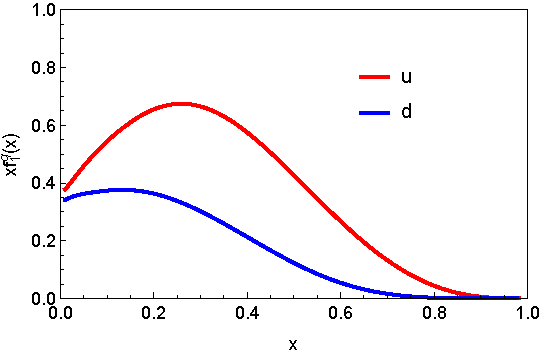
\includegraphics[width=0.4\textwidth]{\FigPath/f1} 
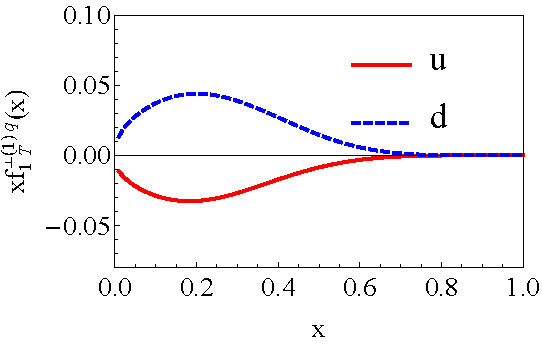
\includegraphics[width=0.4\textwidth]{\FigPath/f1Tperp}
  
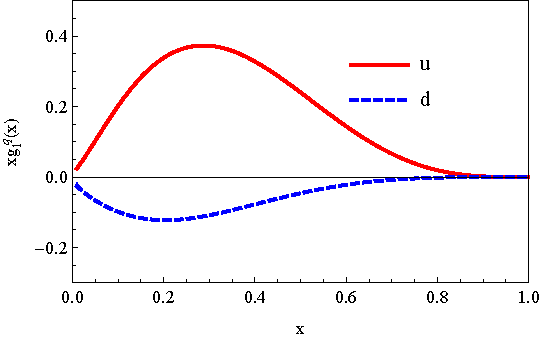
\includegraphics[width=0.4\textwidth]{\FigPath/g1}  
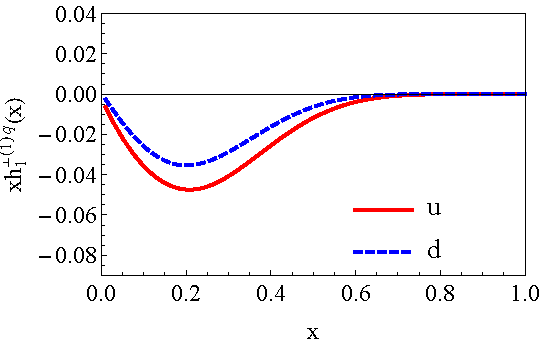
\includegraphics[width=0.4\textwidth]{\FigPath/h1perpBM}  

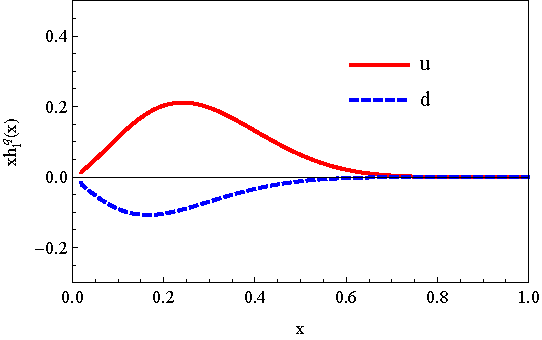
\includegraphics[width=0.4\textwidth]{\FigPath/h1}  
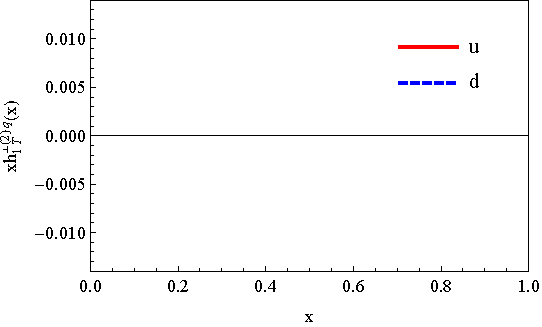
\includegraphics[width=0.4\textwidth]{\FigPath/h1Tperp}


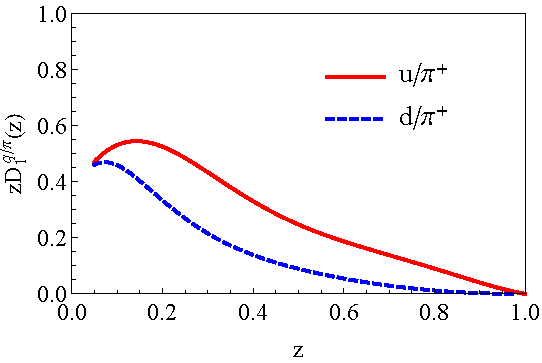
\includegraphics[width=0.4\textwidth]{\FigPath/D1} 
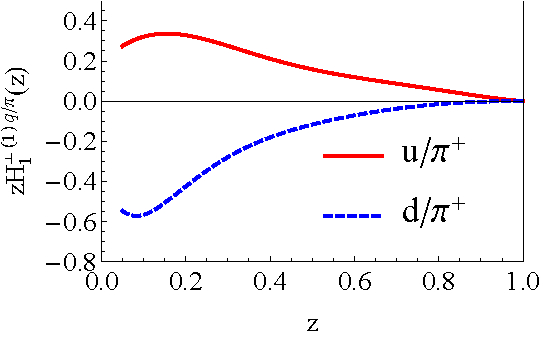
\includegraphics[width=0.4\textwidth]{\FigPath/H1perp} 
\caption{\label{basis} 
	The basis functions $f_1^a, \; g_1^a, \; h_1^a, 
	f_{1T}^{\perp a}, \;h_1^{\perp a},\; h_{1T}^{\perp a}; \; 
	D_1^a, \; H_1^{\perp a} \,$. For details see App.~\ref{App:basis}.}
\end{figure}
%%%%%%%%%%%%%%%%%%%%%%%%%%%%%%%%%%%%%%%%%%%%%%%%%%%%%%%%%%%%%%%%%%%%%%%%%%%%%%%


\subsection{Phenomenological information on basis functions}
\label{Sec-4.3:plot-basis-functions}

We have seen that the following 6 TMDs and 2 FFs provide a basis 
(Sec.~\ref{Sec-3:WW}) and allow us to express all SIDIS structure 
functions (Sec.~\ref{Sec-4:SIDIS-in-WW-approximation})  
in WW-type approximation: 
\be\label{Eq:basis}
   \mbox{basis: \ \ } 
   f_1^a, \; f_{1T}^{\perp a}, \; g_1^a, \; h_1^a, \;h_1^{\perp a},\; h_{1T}^{\perp a};
   \; D_1^a, \; H_1^{\perp a} \, .
\ee
Phenomenological information is available for all basis functions at 
least to some extent. 
In Fig.~\ref{basis} we present plots of the basis functions, and refer
to App.~\ref{App:basis} for details.
The four functions $f_1^a, \; g_1^a, \; h_1^a,\; D_1^a$  
are related to twist-2 collinear functions. All collinear functions are calculated at $Q^2 = 2.4$ (GeV$^2$). Collinear $f_1(x)$ are from Ref.~\cite{Martin:2009iq},  $g_1(x)$ are from Ref.~\cite{Gluck:1998xa}, and $D_1(z)$ are from Ref. ~\cite{deFlorian:2007aj}.The other four 
$f_{1T}^{\perp a},  \;h_1^{\perp a},\; H_1^{\perp a} \,$  
have no collinear counterparts, and we consider their (1)-moments, while 
for $ h_{1T}^{\perp a}$  we consider the (2)-moment,
such that parametrizations of TMD functions read
\begin{subequations}\ba
f^a_1(x,\kperp^2) &=& f^a_1(x)\;
    \frac{e^{-\kperp^2/\avkperp_{f_1}}}{\pi\avkperp_{f_1}} \, ,\\
    D^a_1(z,\pperp^2) &=& D_1^a(z)\,
    \frac{e^{-\pperp^2/\avpperp_{D_1}}}{\pi\avpperp_{D_1}} \, ,\\
g^a_1(x,\kperp^2) &=& g^a_1(x)\;
    \frac{e^{-\kperp^2/\avkperp_{g_1}}}{\pi\avkperp_{g_1}} \, ,\\    
f_{1T}^{\perp q}(x,\kperp^2) &=&  f_{1T}^{\perp (1) q}(x)   \frac{2 M^2}{\pi \avkperp_{f_{1T}^\perp}^2} e^{-\kperp^2/{\avkperp_{f_{1T}^\perp}}} \, ,\\
h_{1}^{q} (x, \kperp^2) &=&h_{1}^{q} (x)  \frac{e^{-{\kperp^2}/{\avkperp_{h_1} }}}{\pi \avkperp_{h_1}}\, ,\\
H_{1}^{\perp}(z,\pperp^2) &=&  H_{1}^{\perp (1)}(z)   \frac{2 z^2 m_h^2}{\pi \avpperp_{H_{1}^\perp}^2} e^{-\pperp^2/{\avpperp_{H_{1}^\perp}}}\, ,\\
h_{1}^{\perp q}(x,\kperp^2) &=&  h_{1}^{\perp (1) q}(x)   \frac{2 M^2}{\pi \avkperp_{h_{1}^\perp}^2} e^{-\kperp^2/{\avkperp_{h_{1}^\perp}}}\, ,\\
h_{1T}^{\perp q}(x,\kperp^2) &=&  h_{1T}^{\perp (2) q}(x)   \frac{2 M^4}{\pi \avkperp_{h_{1T}^\perp}^3} e^{-\kperp^2/{\avkperp_{h_{1T}^\perp}}} \, ,
\ea\end{subequations}
see App.~\ref{App:basis} for details.





%======= SECTION 5: TWIST-2 AND BASIS FUNCTIONS ======================
\section{Leading twist asymmetries and basis functions}
\label{Sec-5:twist-2+basis}
In this section we review how the basis functions describe available
SIDIS data. This is of importance to asses the reliability of the
predictions presented in the next sections.

\subsection{\boldmath Gauss Ansatz and $F_{UU}$ structure function}
\label{Sec-5.1:FUU-basis}

Throughout this work we use the so-called Gauss Ansatz for the
transverse momentum dependent distribution and fragmentation functions. 
This Ansatz is popular not only because it considerably simplifies the
calculations. In fact, all convolution integrals of the type 
(\ref{Eq:def-convolution-integral}) can be solved analytically with 
this Ansatz.
Far more important is the fact that it works phenomenologically
with a good accuracy in many practical applications
\cite{Anselmino:2005nn,Collins:2005ie,D'Alesio:2007jt,Schweitzer:2010tt,
Signori:2013mda,Anselmino:2013lza}.
It should be kept in mind that the Gauss Ansatz can, of course, 
be only a rough approximation. For instance, it is not 
consistent with general matching expectations when $\kperp$ 
becomes large \cite{Bacchetta:2008xw}. Nevertheless, if
one limits oneself to work in a region where the transverse
momenta (of hadrons produced in SIDIS,  dileptons produced
in the Drell-Yan process, etc) are small with respect to the hard
scale in the process, then the Ansatz works quantitatively
very well. The most recent and detailed tests were reported in 
\cite{Schweitzer:2010tt}, where the Gauss Ansatz was shown to
describe the most recent SIDIS data. No deviations could
be observed within the error bars of the data provided one
takes into account the broadening of the Gaussian widths
with increasing energy \cite{Schweitzer:2010tt} according
with expectations from QCD \cite{Aybat:2011zv}.
Remarkably, the Gauss Ansatz is approximately compatible with 
the $\kperp$-shapes obtained from evolution \cite{Aybat:2011zv}
or fits to high-energy Tevatron data on weak-boson production
\cite{Landry:2002ix}. On the other end, effective models at 
low \cite{Pasquini:2008ax,Avakian:2010br} and intermediate 
\cite{Efremov:2009ze} energies also support it approximately.

The Gaussian Ansatz for the unpolarized TMD and unpolarized FF 
is given by
\be\label{Eq:Gauss-f1-D1}
    f^a_1(x,\kperp^2) = f^a_1(x)\;
    \frac{e^{-\kperp^2/\avkperp_{f_1}}}{\pi\avkperp_{f_1}} \;,\;\;\;
    D^a_1(z,\pperp^2) = D_1^a(z)\,
    \frac{e^{-\pperp^2/\avpperp_{D_1}}}{\pi\avpperp_{D_1}}\;.
\ee
The parameters $\avkperp_{f_1}$ and $\avpperp_{D_1}$ can
be assumed to be flavor- and $x$- or $z$-dependent, as present
data do not allow us to constrain too many parameters, see
App.~\ref{App:basis-f1-D1} for a review. This assumption can be
relaxed, e.g. theoretical studies in chiral effective field theories 
predict a strong flavor-dependence in the $\kperp$-behavior
of sea and valence quark TMDs \cite{Schweitzer:2012hh}.

The structure function $F_{UU}$ needed for our analysis reads
\begin{subequations}\ba
	F_{UU}(x,z,\Phperp) 
	&=& x \sum_q e_q^2\,f^q_1(x)\,D_1^q(z)\,{\cal G}(\Phperp)\,, 
	\label{Eq:FUU-Phperp}\\
	F_{UU}(x,z) \equiv \int d^2 \Phperp \, F_{UU}(x,z,\Phperp) 
	&=& x \sum_q e_q^2\,f^q_1(x)\,D_1^q(z)  \, ,
	\label{Eq:FUU}
\ea\end{subequations}
where we introduce the notation ${\cal G}(\Phperp)$, which is defined as
\be\label{Eq:def-Gaussian-lambda}
	{\cal G}(\Phperp) = \frac{\exp(-\Phperp^2/\lambda)}{\pi\,\lambda}
	\, , \;\;\; 
	\lambda = z^2\,\la\kperp^2\ra_{f_1} + \la\pperp^2\ra_{D_1} \,,
\ee
with the understanding that the convenient abbreviation $\lambda$ is expressed 
in terms of the Gaussian widths of the {\it preceding} TMD and FF. Notice 
that ${\cal G}(\Phperp)\equiv {\cal G}(x,z,\Phperp)$ and that in general
${\cal G}(\Phperp)$ appears under the flavor sum due to a possible 
flavor-dependence of the involved Gaussian widths.
The normalization $\int d^2\Phperp \,{\cal G}(\Phperp)=1$ 
correctly connects the structure function $F_{UU}(x,z,\Phperp)$ 
in (\ref{Eq:FUU-Phperp}) with its $\Phperp$-integrated counterpart
(\ref{Eq:FUU}). In our effective description this is step is trivial. In 
QCD the connection of TMDs to PDFs is far more subtle \cite{Collins:2016hqq}.
Fig.~\ref{FUU-show-pT-dependence} illustrates how the Gauss Ansatz
describes selected SIDIS data. In Fig.~\ref{FUU-show-pT-dependence} (b) we plot HERMES multiplicity \cite{Airapetian:2012ki}
\be
M_n^h(x,z,\Phperp)  \equiv 2 \pi \Phperp \frac{F_{UU}(x,z,\Phperp) }{ x \sum_q e_q^2\,f^q_1(x)}
\ee
at $\la Q^2\ra=2.87\,{\rm GeV}^2$,
$\la x\ra  =0.15$, $\la z\ra  =0.22$ for $\pi^+$ production on the proton target.
In Fig.~\ref{FUU-show-pT-dependence} (c) we plot COMPASS multiplicity \cite{Aghasyan:2017ctw}
\be
n^h(x,z,\Phperp)  \equiv \pi \frac{F_{UU}(x,z,\Phperp) }{ x \sum_q e_q^2\,f^q_1(x)}
\ee
at $\la Q^2\ra=20\,{\rm GeV}^2$,
$\la x\ra  =0.15$, $\la z\ra  =0.2$ for $h^+$ production on the deuterium target.

To streamline the presentation we refer to the comprehensive Appendix 
on the used parametrizations (App.~\ref{App:basis}), and for 
technical details on the Gauss Ansatz (App.~\ref{App:factor}).

%%%%%%%%%%%%%%%%%%%%%%%%%%%%%%%%%%%%%%%%%%%%%%%%%%%%%%%%%%%%%%%%%%%%%%%%%%%%%%%
\begin{figure}[t!]
\centering
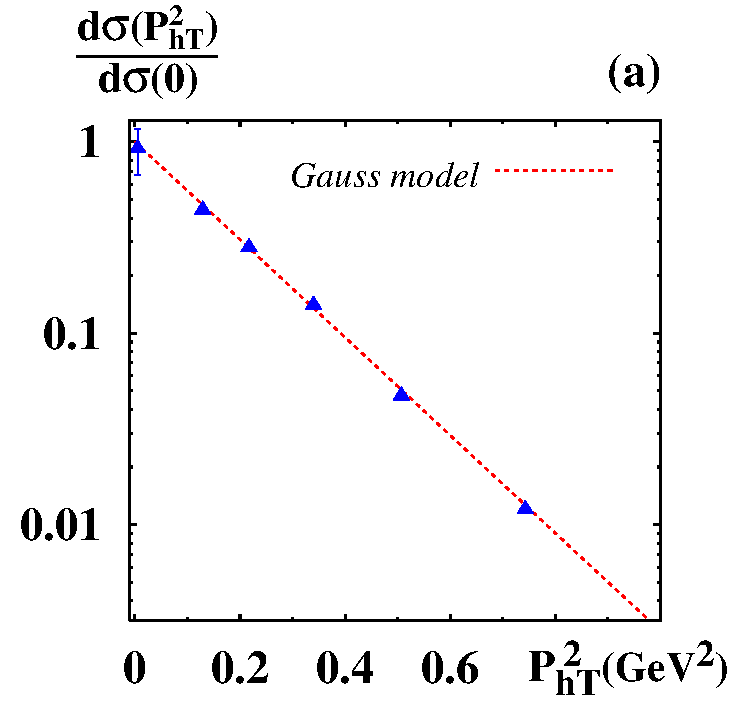
\includegraphics[width=0.3\textwidth]{\FigPath/Fig02a-JLab-ratio-pT-v5.pdf}  (a)
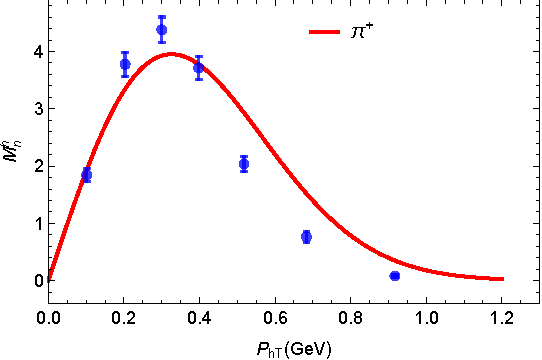
\includegraphics[width=0.37\textwidth]{\FigPath/hermes_pip.pdf} (b)
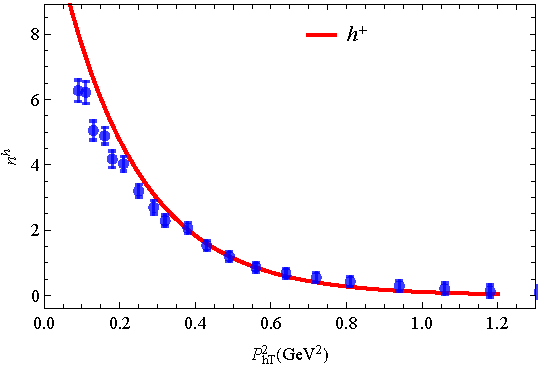
\includegraphics[width=0.37\textwidth]{\FigPath/compass_hp.pdf} (c)
\caption{\label{FUU-show-pT-dependence}
Examples of the description of transverse momenta of hadrons in 
unpolarized SIDIS. 
(a) Differential cross section at $\la Q^2\ra=2.37\,{\rm GeV}^2$,
$\la x\ra  =0.24$, $\la z\ra  =0.30$ measured at JLab with a 5.75 GeV 
beam \cite{Osipenko:2008aa}. Theoretical curve from Gauss model 
following Ref.~\cite{Schweitzer:2010tt}.
(b) Example for HERMES multiplicities \cite{Airapetian:2012ki} at $\la Q^2\ra=2.87\,{\rm GeV}^2$,
$\la x\ra  =0.15$, $\la z\ra  =0.22$.
(b) Example for COMPASS multiplicities \cite{Aghasyan:2017ctw} at $\la Q^2\ra=20\,{\rm GeV}^2$,
$\la x\ra  =0.15$, $\la z\ra  =0.2$.}
\end{figure}
%%%%%%%%%%%%%%%%%%%%%%%%%%%%%%%%%%%%%%%%%%%%%%%%%%%%%%%%%%%%%%%%%%%%%%%%%%%%%%%



%\newpage
%========= SECTION 6: TESTING APPROACH WITH A_LL =====================
\subsection{\boldmath Leading twist $A_{LL}$: 
           first test of intrinsic $\kperp$ beyond unpolarized case}
\label{Sec-5.2:FLL-basis}

In this Section we discuss the leading twist double spin asymmetry 
$A_{LL} \propto g_{1}^a D_1^a$ which does not require a WW-type approximation
but is important for two reasons. First, we review one of our 
``basis functions'' $g_1^a(x)$, and similarly we will review below 
also other ``basis functions.'' Second, throughout this work we use the 
Gaussian Ansatz demonstrated to provide good services in unpolarized case 
\cite{Anselmino:2005nn,Collins:2005ie,D'Alesio:2007jt,Schweitzer:2010tt,
Signori:2013mda,Anselmino:2013lza}. However, nothing is known about
the applicability of the Gaussian Ansatz in polarized case.
The JLab data \cite{Avakian:2010ae} on $A_{LL}(\Phperp)$ put us 
in the position to conduct a first ``test'' of our understanding of 
the $\kperp$-behavior of polarized partons. To have an ``informed idea''
about the Gaussian width of $g_{1}(x,\kperp)$ we will explore information
from the exploratory lattice QCD study of TMDs \cite{Hagler:2009mb}.

We assume Gaussian form for $g_{1}^{a}(x,\kperp^2)$
\ba\label{eq:g1}
	g_{1}^{a}(x,\kperp^2) = g_{1}^{a}(x)\,
	\frac{e^{-\kperp^2/{\avkperp_{g_{1}}}}}{\pi \avkperp_{g_{1}}}\,\; ,
\ea
and resort to the lattice QCD results \cite{Hagler:2009mb} to gain 
an estimate on width $\avkperp_{g_{1}}$, see App.~\ref{App:basis-g1}.

With $\lambda=z^2\la\kperp^2\ra_{g_1}+\la\pperp^2\ra_{D_1}$ implicit in 
${\cal G}(\Phperp)$, the structure function $F_{LL}$  reads
\begin{subequations}\ba
	F_{LL}(x,z,\Phperp) 
	&=& x \sum_q e_q^2\,g^q_1(x)\,D_1^q(z)\,{\cal G}(\Phperp)\,, 
	\label{Eq:FLL-Phperp}\\
	F_{LL}(x,z)  
	&=& x \sum_q e_q^2\,g^q_1(x)\,D_1^q(z)  \, ,
	\label{Eq:FLL}
\ea\end{subequations}




%%%%%%%%%%%%%%%%%%%%%%%%%%%%%%%%%%%%%%%%%%%%%%%%%%%%%%%%%%%%%%%%%%%%%%%%%%%%%%%
\begin{figure}[t]
\centering 
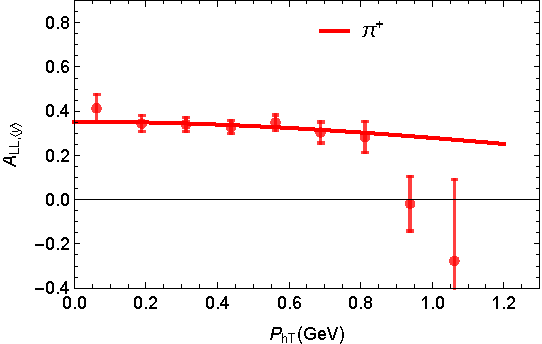
\includegraphics[width=0.32\textwidth]{\FigPath/all_jlab_pip}  
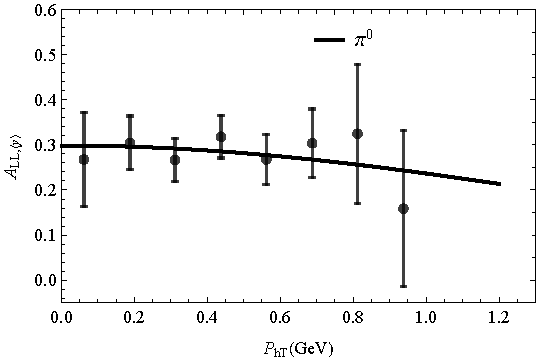
\includegraphics[width=0.32\textwidth]{\FigPath/all_jlab_pi0}  
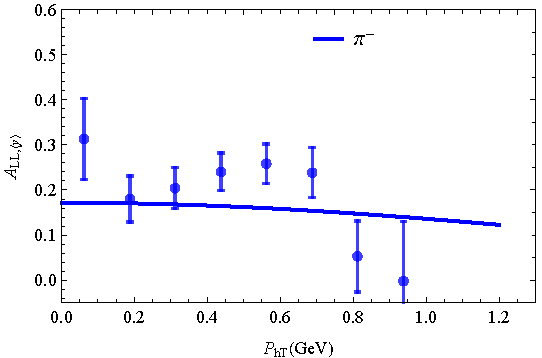
\includegraphics[width=0.32\textwidth]{\FigPath/all_jlab_pim}  
\caption{\label{jlab_ALL} 
	$A_{LL,\la y\ra}$ asymmetry compared with Jefferson Lab experimental 
	results Ref.~\cite{Avakian:2010ae} for $\pi^+$ (left panel) and 
	$\pi^-$ (right panel). Solid lines are computations with mean 
	values of kinematic variables  $\langle x \rangle = 0.25$, 
	$\langle z \rangle = 0.5$, $\langle Q^2 \rangle = 1.7$ GeV$^2$.
}
\end{figure}
%%%%%%%%%%%%%%%%%%%%%%%%%%%%%%%%%%%%%%%%%%%%%%%%%%%%%%%%%%%%%%%%%%%%%%%%%%%%%%%

The first experimental results on the 
$\Phperp$-dependence of $A_{LL} = F_{LL}/F_{UU}$ were presented by
Jefferson Lab \cite{Avakian:2010ae}. The definition of the asymmetry 
in  \cite{Avakian:2010ae} was
\be\label{Eq:ALLy}
	A_{LL,\la y\ra}(x,z,\Phperp) 
	= \la p_2 \,A_{LL}(x,z,\Phperp) \ra \, 
	= \frac{\la y (2-y) \; F_{LL}(x,z,\Phperp)\ra}
	{\la(1+(1-y)^2) \; F_{UU}(x,z,\Phperp)\ra} 
\ee 
where $p_2 = y (2-y)/(1+(1-y)^2)$ and averaging (separately in numerator 
and denominator) over the kinematics of \cite{Avakian:2010ae} is implied. 
We  compare our results for $A_{LL,\la y\ra}(\Phperp)$ to Jefferson Lab data 
\cite{Avakian:2010ae} in Fig.~\ref{jlab_ALL}.

In our approach we use lattice results from \cite{Hagler:2009mb} to
constrain the Gaussian width $\la\kperp^2\ra_{g_1}$, see App.~\ref{App:basis-g1}.
All other ingredients in (\ref{Eq:ALLy}) are known and 
tested through other observables, see Sec.~\ref{Sec-5.1:FUU-basis}.
Therefore Fig.~\ref{jlab_ALL} provides several important tests.
First, the Jefferson Lab data \cite{Avakian:2010ae} is compatible
with the Gauss Ansatz within error bars. Second, the lattice QCD results 
in the way we use them in App.~\ref{App:basis-g1} give an appropriate 
description of these data.\footnote{
	Another important test was already presented in 
	\cite{Avakian:2010ae}: the $\Phperp$-integrated (``collinear'')
	asymmetry (\ref{Eq:FLL}) is compatible with data
	from other experiments and with theoretical results obtained from
	parametrizations of $f_1^a(x)$, $g_1^a(x)$, $D_1^a(z)$. This 
	shows that even at the moderate beam energies of the pre-12GeV era 
	one was indeed already probing DIS at Jefferson Lab,
	at least to a very good approximation \cite{Avakian:2010ae}.}

Encouraged by these findings we will use lattice predictions from 
Ref.~\cite{Hagler:2009mb} below also for the Gaussian widths of 
$g_{1T}^{\perp(1)a}$ and $h_{1L}^{\perp(1)a}$.
Of course, at this point one could argue that the WW- and WW-type 
approximations (\ref{Eq:WW-approx-g1T},~\ref{Eq:WW-approx-g1T}) also
dictate that $g_{1T}^\perp$ and $h_{1L}^\perp$ have the same Gaussian
widths as $g_1$ and $h_1$. In fact, the lattice results for the 
respective widths are numerically similar, which can be interpreted as 
yet another argument in favor of the usefulness of the approximations. 
The practical predictions depend only weakly on the choice of parameters.

\newpage
\subsection{\boldmath Leading twist $A_{UT}^{\sin(\phi_h-\phi_S)}$ Sivers asymmetry}
\label{Sec-5.3:Sivers-basis}

The $F_{UT}^{\sin(\phi_h-\phi_S)}$ modulation of SIDIS cross section is related to  the Sivers function~\cite{Sivers:1989cc}, which describes the number density of unpolarized quarks inside a 
transversely polarized proton, has so far received the widest attention, 
from both phenomenological and experimental points of view. 

The Sivers function $f_{1T}^\perp$ is related to initial and final state interactions of the struck quark and the rest of the nucleon and could not exist 
without the contribution of the orbital angular momentum of partons to the spin of the nucleon. 
As such it encodes the correlation between the partonic intrinsic motion and the transverse spin of the nucleon, and it generates a dipole deformation in momentum space.

Over the years, the Sivers function has been extracted from SIDIS data
by several groups, with consistent results 
\cite{Anselmino:2010bs,Anselmino:2005ea,Anselmino:2005an,Collins:2005ie,Vogelsang:2005cs,Anselmino:2008sga,Bacchetta:2011gx,Echevarria:2014xaa}. 

The structure function $F_{UT}^{\sin(\phi_h-\phi_S)}$ reads
\begin{subequations}\ba
	F_{UT}^{\sin(\phi_h-\phi_S)}(x,z,\Phperp) 
	&=& - x\sum_q e_q^2\,f_{1T}^{\perp (1) q}(x)\,D_1^{q}(z)\; 
	b^{(1)}_{\rm B}\,\biggl(\frac{z \Phperp} {\lambda}\biggr)\,
	{ \cal G}(\Phperp ) \, , \label{FUTsiv-Gauss-Phperp}\\ 
	F_{UT}^{\sin(\phi_h-\phi_S)}(x,z,\la\Phperp\ra) 
	&=& - x\sum_q e_q^2\,f_{1T}^{\perp (1) q}(x)\,D_1^{q}(z)\;
	c^{(1)}_{\rm B}\,\biggl(\frac{z} {\lambda^{1/2}}\biggr)\,,\label{FUTsiv-Gauss}
\ea\end{subequations}
where $\lambda=z^2 \avkperp_{f_{1T}^\perp} + \avpperp_{D_1}$ and
$b^{(1)}_{\rm B}=2M_N$ and $c^{(1)}_{\rm B} = \sqrt{\pi}\,M_N$, 
see App.~\ref{App:convol-details} for details.

Notice that integrating structure functions over $\Phperp$
is different from integrating the cross section over $\Phperp$
where azimuthal hadron modulations drop out. 
Only if the relevant weight is $\omega^{\{0\}}$ we obtain
``collinear structure functions:''  $F_{UU}(x,z)$, $F_{LL}(x,z)$ 
in Secs.~\ref{Sec-5.1:FUU-basis}, \ref{Sec-5.2:FLL-basis}
and below in Secs.~\ref{Sec-7.2:FLTcosphiS}, \ref{Sec-7.6:FUTsinphiS}.
In all other cases, despite integration over $\Phperp$, we end up 
always with true convoluted TMDs (here within Gauss model).
We stress this important point by displaying the dependence of 
the structure functions on the mean hadron momenta, for instance
$F_{UT}^{\sin(\phi_h-\phi_S)}(x,z,\la\Phperp\ra) = 
\int d^2\Phperp F_{UT}^{\sin(\phi_h-\phi_S)}(x,z,\Phperp)$
in (\ref{FUTsiv-Gauss}).




The asymmetries $A_{UT}^{\sin(\phi_h-\phi_S)}= F_{UT}^{\sin(\phi_h-\phi_S)}/F_{UU}$  
and comparison to HERMES data \cite{Airapetian:2009ae} are plotted in Fig.~\ref{aut_f1t_jlab}.



%%%%%%%%%%%%%%%%%%%%%%%%%%%%%%%%%%%%%%%%%%%%%%%%%%%%%%%%%%%%%%%%%%%%%%%%%%%%%%%
\begin{figure}[b!]
\centering
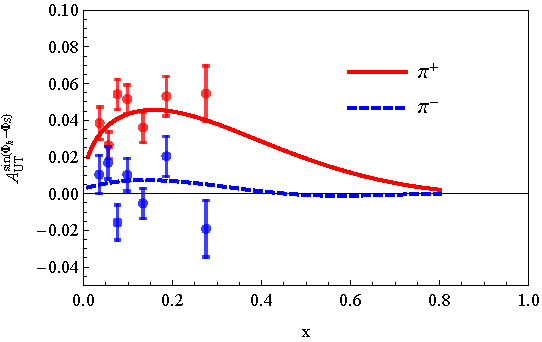
\includegraphics[width=0.45\textwidth]{\FigPath/AUTSivers_x.pdf}  
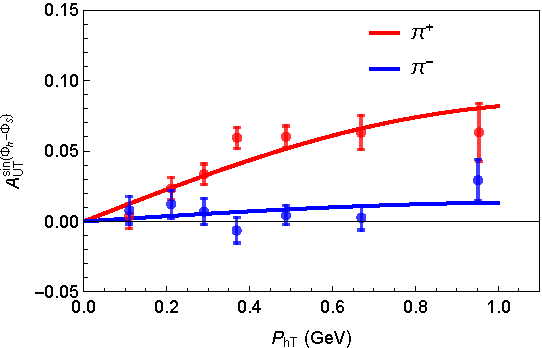
\includegraphics[width=0.45\textwidth]{\FigPath/AUTSivers_PT.pdf}
\caption{\label{aut_f1t_jlab} Comparison of calculation of $A_{UT}^{\sin(\phi_h-\phi_S)}$  using fit results of Ref.~\cite{Anselmino:2011gs} as a function of $ x $ (left panel), and   as a function of $P_{hT}$ (right panel) at $\la x\ra = 0.15$, $\la z\ra = 0.34$, $\la Q^2\ra = 2.4$ GeV$^2$ and HERMES data \cite{Airapetian:2009ae}.
}
\end{figure}
%%%%%%%%%%%%%%%%%%%%%%%%%%%%%%%%%%%%%%%%%%%%%%%%%%%%%%%%%%%%%%%%%%%%%%%%%%%%%%%

\newpage

\subsection{\boldmath Leading twist $A_{UT}^{\sin(\phi_h+\phi_S)}$ Collins asymmetry}
\label{Sec-5.4:Collins-basis}

The $F_{UT}^{\sin(\phi_h+\phi_S)}$ modulation of the SIDIS cross section is due to convolution of the transversity distribution $h_1$, which is the only source of information on the tensor charge of the 
nucleon, and the Collins FF $H_1^\perp$, that decodes the fundamental correlation between
the transverse spin of a fragmenting quark and the transverse momentum
of the final produced hadron. 

There are many extractions of $h_1$ and $H_1^\perp$ from a combined fit of SIDIS and $e^+e^-$ data, for instance those of Refs.~\cite{Anselmino:2013vqa,Kang:2014zza,Anselmino:2015sxa}.


The structure function $F_{UT}^{\sin(\phi_h+\phi_S)}$ reads
\begin{subequations}\ba
	F_{UT}^{\sin(\phi_h+\phi_S)}(x,z,\Phperp) 
	&=& x\sum_q e_q^2\,h_{1}^{q}(x)\,H_1^{\perp(1)q}(z)\; 
	b^{(1)}_{\rm A}\,\biggl(\frac{z \Phperp} {\lambda}\biggr)\,
	{ \cal G}(\Phperp ) \, , \\
	F_{UT}^{\sin(\phi_h+\phi_S)}(x,z,\la\Phperp\ra) 
	&=& x\sum_q e_q^2\,h_{1}^{q}(x)\,H_1^{\perp(1)q}(z)\;  
	c^{(1)}_{\rm A}\,\biggl(\frac{z} {\lambda^{1/2}}\biggr)\,,
	\label{eq:asymmetry_aut_h1}
\ea\end{subequations}
where $\lambda=z^2 \avkperp_{h_1} + \avpperp_{H_1^\perp}$ and
$b^{(1)}_{\rm A}=2m_h$ and $c^{(1)}_{\rm A} = \sqrt{\pi}\,m_h$,
see App.~\ref{App:convol-details} for details.

The asymmetries $A_{UT}^{\sin(\phi_h+\phi_S)}=F_{UT}^{\sin(\phi_h+\phi_S)}/F_{UU}$
and comparison to HERMES data \cite{Airapetian:2010ds} are plotted in Fig.~\ref{aut_h1_jlab}.




%%%%%%%%%%%%%%%%%%%%%%%%%%%%%%%%%%%%%%%%%%%%%%%%%%%%%%%%%%%%%%%%%%%%%%%%%%%%%%%
\begin{figure}[b!]
\centering
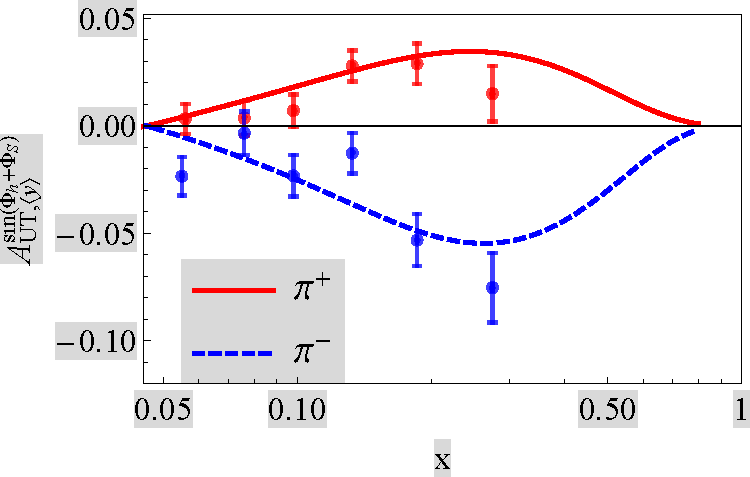
\includegraphics[width=0.45\textwidth]{\FigPath/AUTCollins_x.pdf}  
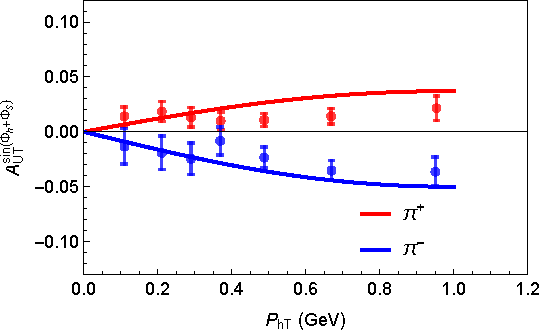
\includegraphics[width=0.45\textwidth]{\FigPath/AUTCollins_PT.pdf}
\caption{\label{aut_h1_jlab} Comparison of calculation of $A_{UT}^{\sin(\phi_h+\phi_S)}$  using fit results of Ref.~\cite{Anselmino:2013vqa} as a function of $ x $ (left panel), and   as a function of $P_{hT}$ (right panel) at $\la x\ra = 0.15$, $\la z\ra = 0.34$, $\la Q^2\ra = 2.4$ GeV$^2$ and HERMES data \cite{Airapetian:2009ae}.
}
\end{figure}
%%%%%%%%%%%%%%%%%%%%%%%%%%%%%%%%%%%%%%%%%%%%%%%%%%%%%%%%%%%%%%%%%%%%%%%%%%%%%%%

\newpage
\subsection{\boldmath Leading twist $A_{UU}^{\cos(2\phi_h)}$ Boer-Mulders asymmetry}
\label{Sec-5.5:BM-basis}

The structure function $F_{UU}^{\cos(2\phi_h)}$ reads
\begin{subequations}\ba
	F_{UU}^{\cos(2\phi_h)}(x,z,\Phperp) 
	&=& x \sum_q e_q^2\,h_{1}^{\perp (1) q}(x)\,H_1^{\perp(1) q}(z)\; 
	b^{(2)}_{\rm AB}\,\biggl(\frac{z \Phperp} {\lambda}\biggr)^{\!2}\,
	{ \cal G}(\Phperp)\, , \\
	F_{UU}^{\cos2\phi_h}(x,z,\la\Phperp\ra) 
	&=& x\sum_q e_q^2\,h_{1}^{\perp(1) q}(x)\,H_1^{\perp(1)q}(z)\;  
	c^{(2)}_{\rm AB}\,\biggl(\frac{z} {\lambda^{1/2}}\biggr)^{\!2}\,,
	\label{eq:asymmetry_auu_cos2phi}
\ea\end{subequations}
where $\lambda=z^2 \avkperp_{h_1^\perp} + \avpperp_{H_1^\perp}$ and
$b^{(2)}_{\rm AB}=4M_Nm_h$ and $c^{(2)}_{\rm AB} = 4M_Nm_h$,
see App.~\ref{App:convol-details}.



%%%%%%%%%%%%%%%%%%%%%%%%%%%%%%%%%%%%%%%%%%%%%%%%%%%%%%%%%%%%%%%%%%%%%%%%%%%%%%%
\begin{figure}[b!]
\centering
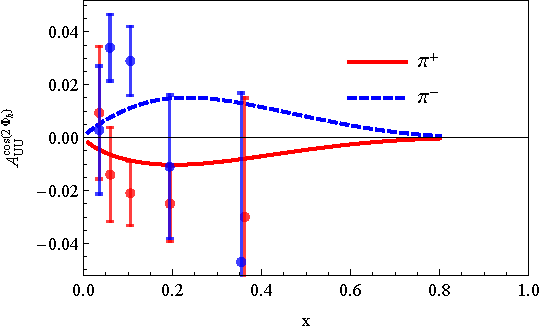
\includegraphics[width=0.45\textwidth]{\FigPath/AUUcos2phi_x.pdf} 
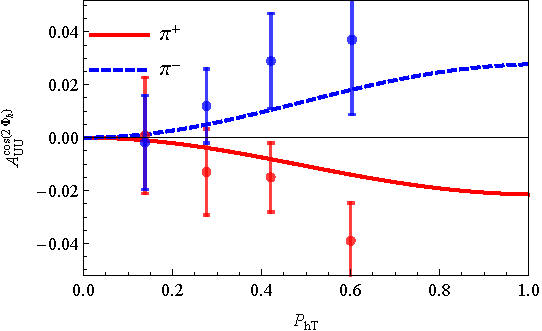
\includegraphics[width=0.45\textwidth]{\FigPath/AUUcos2phi_PT.pdf}
\caption{\label{auu_cos2phi_jlab} Comparison of calculation of $A_{UU}^{\cos(2\phi_h)}$  using fit results of Ref.~\cite{Barone:2015ksa} as a function of $ x $ (left panel), and   as a function of $P_{hT}$ (right panel) at $\la x\ra = 0.15$, $\la z\ra = 0.34$, $\la Q^2\ra = 2.4$ GeV$^2$ and HERMES data \cite{Giordano:2009hi}.
}
\end{figure}
%%%%%%%%%%%%%%%%%%%%%%%%%%%%%%%%%%%%%%%%%%%%%%%%%%%%%%%%%%%%%%%%%%%%%%%%%%%%%%%

Asymmetries $A_{UU}^{\cos(2\phi_h)}=F_{UU}^{\cos(2\phi_h)}/F_{UU}$  for  
HERMES are plotted in Fig.~\ref{auu_cos2phi_jlab}.
In the Fig.~\ref{auu_cos2phi_jlab} we plot only the
Boer-Mulders contribution to $A_{UU}^{\cos(2\phi_h)}$ which does not describe
the data accurately. In fact, it is suspected that this observable receives 
a significant contribution from the Cahn effect \cite{Cahn:1978se}, a 
term of higher twist character of the type $\la\Phperp^2\ra/Q^2$ which 
is not negligible in fixed target experiments \cite{Schweitzer:2010tt}. 
This contribution was estimated and corrected for in the phenomenological 
works \cite{Barone:2009hw,Barone:2010gk,Barone:2015ksa} which was of
importance to obtain a picture of the Boer-Mulders function undistorted 
from Cahn effect. The point is that this substantial twist-4 contamination 
can be estimated phenomenologically, even though there is no rigorous 
theoretical basis for the description of such power-suppressed terms. 
In this work we consistently neglect power-suppressed contributions of 
order $1/Q^2$, and do so also in Fig.~\ref{auu_cos2phi_jlab}. 
Nevertheless we of course use the parametrizations of 
\cite{Barone:2009hw,Barone:2010gk,Barone:2015ksa} offering
the best currently available parametrizations for $h_1^{\perp}$
which were corrected for Cahn effect as good as it is possible at
the current stage of art. It is unknown whether other asymmetries
could be similarly effected by such type of power-corrections.
This is an important point to be kept in mind as the lesson 
from Fig.~\ref{auu_cos2phi_jlab} shows.


\newpage
\subsection{\boldmath Leading twist $A_{UT}^{\sin(3\phi_h-\phi_S)}$  asymmetry}
\label{Sec-5.6:pretzel-basis}

The structure function $F_{UT}^{\sin(3\phi_h-\phi_S)}$ reads
\begin{subequations}\ba
	F_{UT}^{\sin(3\phi_h-\phi_S)}(x,z,\Phperp)
	&=& x \sum_q e_q^2\,h_{1T}^{\perp (2) q}(x)\,H_1^{\perp(1) q}(z)\; 
	b^{(3)}\,\biggl(\frac{z \Phperp} {\lambda}\biggr)^{\!3}\,
	{ \cal G}(\Phperp) \, , \;\;\;\;
	\label{eq:asymmetry_aut_h1tp} \\
	F_{UT}^{\sin(3\phi_h-\phi_S)}(x,z,\la\Phperp\ra) 
	&=& x\sum_q e_q^2\,h_{1T}^{\perp (2) q}(x)\,H_1^{\perp(1)q}(z)\;  
	c^{(3)}\,\biggl(\frac{z} {\lambda^{1/2}}\biggr)^{3}\,,
\ea\end{subequations}
where $\lambda=z^2 \avkperp_{h_{1T}^\perp} + \avpperp_{H_1^\perp}$ and
$b^{(3)}=2M_N^2m_h$ and $c^{(3)}_{\rm  } = 3/2\sqrt{\pi} \,M_N^2m_h$,
see App.~\ref{App:convol-details}.

Asymmetries $A_{UT}^{\sin(3 \phi_h - \phi_S)}=F_{UT}^{\sin(3 \phi_h - \phi_S)}/F_{UU}$ for 
COMPASS data \cite{Parsamyan:2010se} are plotted in Fig.~\ref{aut_h1tp_jlab}.
Clearly, the pretzelosity TMD is the least known of the basis TMDs.
Nevertheless it is of fundamental importance, as it provides one of the
basis functions in our approach. It is so difficult to access it 
experimentally, because its contribution to the SIDIS cross section
is proportional to $\Phperp^3$, the TMD approach requires us to
necessarily operate at $\Phperp\ll Q$, and so far only moderate
values of $Q$ could be achieved in the fixed target experiments.
A notable exception is COMPASS where the largest $x$-bins 
(where $Q^2$ is largest) bear the best hints on this TMD,
see Fig.~\ref{aut_h1tp_jlab}.
Future high luminosity data from Jefferson Lab 12 are expected 
to significantly improve our knowledge of this TMD.


%%%%%%%%%%%%%%%%%%%%%%%%%%%%%%%%%%%%%%%%%%%%%%%%%%%%%%%%%%%%%%%%%%%%%%%%%%%%%%%
\begin{figure}[b!]
\centering
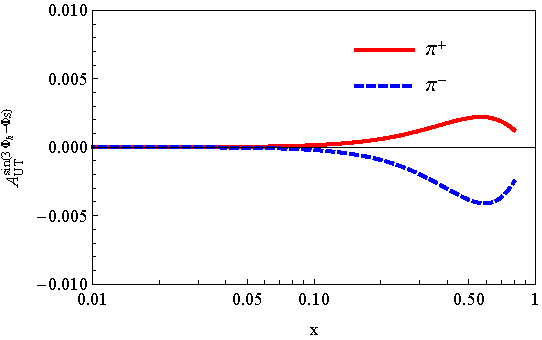
\includegraphics[width=0.45\textwidth]{\FigPath/AUTPretzelosity_x.pdf}  
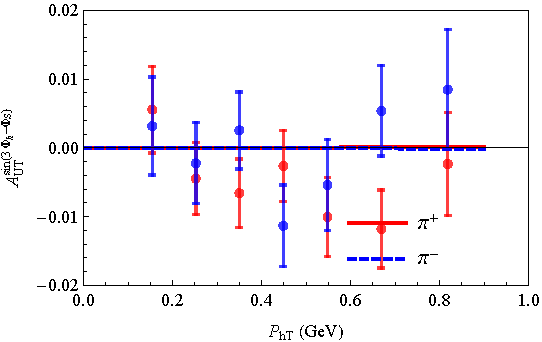
\includegraphics[width=0.45\textwidth]{\FigPath/AUTPretzelosity_PT.pdf}
\caption{\label{aut_h1tp_jlab}  Comparison of calculation of $A_{UT}^{\sin(3 \phi_h - \phi_S)}$  using fit results of Ref.~\cite{Lefky:2014eia} as a function of $ x $ (left panel), and   as a function of $P_{hT}$ (right panel) at $\la x\ra = 0.15$, $\la z\ra = 0.34$, $\la Q^2\ra = 2.4$ GeV$^2$ and preliminary COMPASS data \cite{Parsamyan:2010se}.
}
\end{figure}
%%%%%%%%%%%%%%%%%%%%%%%%%%%%%%%%%%%%%%%%%%%%%%%%%%%%%%%%%%%%%%%%%%%%%%%%%%%%%%%


\newpage
%======= SECTION 6: TWIST-2 AND WW-APROXIMATION ======================
\section{Leading twist asymmetries in WW-type approximation}
\label{Sec-6:twist-2-and-WW}

Two out of the 8 leading-twist structure functions can be 
described in the WW-type approximation thanks to the relations 
(\ref{Eq:WW-approx-g1T},~\ref{Eq:WW-approx-h1L}) which allow us
to express $g_{1T}^{\perp (1) q}(x)$ and $h_{1L}^{\perp (1) q}(x)$ on 
the basis of available information on $g_1^q(x)$ and $h_1^a(x)$,
see Fig.~\ref{g1t_h1l_functions}.
In this section we discuss the associated asymmetries.

\begin{figure}[h!]
\centering
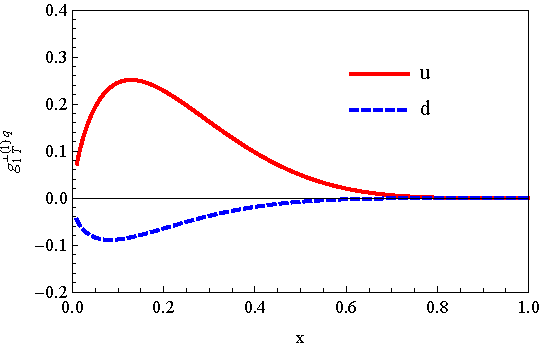
\includegraphics[width=0.45\textwidth]{\FigPath/g1t.pdf} 
\includegraphics[width=0.45\textwidth]{\FigPath/h1lperp.pdf}
	\caption{\label{g1t_h1l_functions} 
	$g^{\perp (1) q}_{1T}(x)$ (left panel) and
	$h^{\perp (1) q}_{1L}(x)$ distributions (right panel) for 
	$u$- and $d$-flavor. 
}
\end{figure}

\subsection{\boldmath Leading twist $A_{LT}^{\cos(\phi_h-\phi_S)}$}
\label{Sec-6.1:FLTcosphi-phiS}

We assume for $g^{\perp}_{1T}$ the Gaussian Ansatz as follows 
\cite{Kotzinian:2006dw} 
\be
	g^{\perp q}_{1T}(x,\kperp^2) = 
	g^{\perp (1) q}_{1T}(x)\,\frac{2 M^2}{\pi \avkperp_{g_{1T}^\perp}^2}\,
	e^{-\kperp^2/{\avkperp_{g_{1T}^\perp}}}\;,
	\label{eq:g1t}
\ee
and evaluate $g^{\perp (1) q}_{1T}(x)$ using Eq.~(\ref{Eq:WW-approx-g1T})
which yields the result shown in Fig.~\ref{g1t_h1l_functions}.
For our numerical estimates we use $\avkperp_{g_{1T}^\perp} = \avkperp_{g_{1}}$ 
which is supported by lattice results \cite{Hagler:2009mb}.

In the Gauss Ansatz the structure function $F_{LT}^{\cos(\phi_h -\phi_S)}$ 
has the form
\begin{subequations}\ba
	F_{LT}^{\cos(\phi_h -\phi_S)}(x,z,\Phperp) 
	&=& x\sum_q e_q^2\,g_{1T}^{\perp (1) q}(x)\,D_1^{q}(z)\; 
	b^{(1)}_{\rm B}\,\biggl(\frac{z \Phperp} {\lambda}\biggr)\,
	{ \cal G}(\Phperp ) \\
	F_{LT}^{\cos(\phi_h-\phi_S)}(x,z,\la\Phperp\ra) 
	&=&  x\sum_q e_q^2\,g_{1T}^{\perp (1) q}(x)\,D_1^{q}(z)\;
	c^{(1)}_{\rm B}\,\biggl(\frac{z} {\lambda^{1/2}}\biggr)\,
	\label{eq:asymmetry_g1t_pt-II}
\ea\end{subequations}
where 
$\lambda  = z^2 \avkperp_{g_{1T}^\perp} + \avpperp_{D_1}$,
$b^{(1)}_{\rm B} = 2M_N$,
$c^{(1)}_{\rm B} = \sqrt{\pi}\,M_N$,
see App.~\ref{App:convol-details} for details.
The $g^{\perp q}_{1T}$ and the Sivers function $f^{\perp q}_{1T}$ are both 
constrained by the positivity bound \cite{Bacchetta:1999kz} 
\be
	\frac{\kperp^2}{M^2}\left( (g^{\perp q}_{1T}(x,\kperp^2))^2 
	+ (f_{1T}^{\perp q}(x,\kperp^2))^2\right) \le (f_{1}^{q}(x,\kperp^2))^2 
\ee
so that using our Gaussian parametrizations from Eqs.~(\ref{Eq:Gauss-f1-D1},\ref{eq:g1t},\ref{sivers_new}) one has
\be
\frac{(f_{1}^{q}(x))^2}{16\pi M^2} - \frac{(f_{1T}^{\perp q}(x))^2}{4\pi \avkperp_{f_{1T}^\perp} } -
\frac{(g_{1T}^{\perp q}(x))^2}{4\pi \avkperp_{g_{1T}^\perp} } \ge 0
\label{eq:positivity}
\ee
see Fig.~\ref{g1t_pos} where RHS of this equation multiplied by $16\pi M^2$ is shown.

%%%%%%%%%%%%%%%%%%%%%%%%%%%%%%%%%%%
\begin{figure}[h!]
\centering
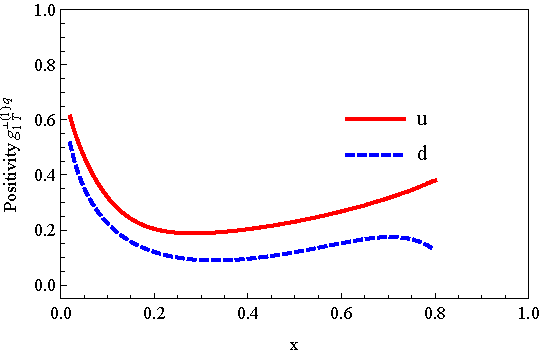
\includegraphics[width=0.45\textwidth]{\FigPath/g1t_positivity.pdf}  
	\caption{\label{g1t_pos} 
	LHS of Eq.~\eqref{eq:positivity}.
}
\end{figure}
%%%%%%%%%%%%%%%%%%%%%%%%%%%%%%%%%%%%%%%%%%%%

%%%%%%%%%%%%%%%%%%%%%%%%%%%%%%%%%%%%%%%%%%%%%%%%%%%%%%%%%%%%%%%%%%%%%%%%%%%%%%%
\begin{figure}[h!]
\centering
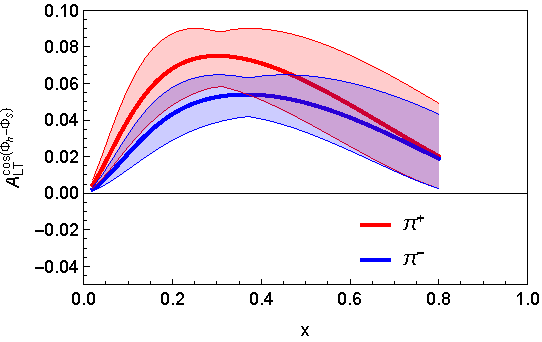
\includegraphics[width=0.45\textwidth]{\FigPath/ALT_COMPASS_x.pdf}  
	\caption{\label{g1t_jlab} 
	$A_{LT}^{\cos(\phi_h -\phi_S)}$  as a function of $ x $  at typical kinematics 
	of COMPASS, 
	$\la x\ra = 0.05$, $\la z\ra = 0.36$, $\la Q^2\ra = 2.4$ GeV$^2$.
	\newline\PS{Can we compare here to COMPASS data from 
	\cite{Kotzinian:2007uv}?}}
\end{figure}
%%%%%%%%%%%%%%%%%%%%%%%%%%%%%%%%%%%%%%%%%%%%%%%%%%%%%%%%%%%%%%%%%%%%%%%%%%%%%%%

The asymmetry  $A_{LT}^{\cos(\phi_h -\phi_S)}$ as a function of $x$  
for COMPASS is plotted in Fig.~\ref{g1t_jlab}.


\newpage
\subsection{\boldmath 
	Leading twist $A_{UL}^{\sin2\phi_h}$ Kotzinian-Mulders  asymmetry}
\label{Sec-6.2:FULsin2phi}


We assume Gaussian form for Kotzinian-Mulders function $h_{1L}^{\perp a}$:
\be
	h_{1L}^{\perp a}(x,\kperp^2) = h_{1L}^{\perp (1) a}(x)\,
	\frac{2 M^2}{\pi{\avkperp_{h_{1L}^\perp}^2}}\,e^{-\kperp^2/{\avkperp_{h_{1L}^\perp}^2}}
	\;,\label{eq:h1l_final}
\ee
We will use WW-type approximation from Eq.~(\ref{Eq:WW-approx-h1L}) 
for calculation of $h_{1L}^{\perp (1) a}(x)$ and for the estimates of the 
asymmetry $\avkperp_{h_{1L}^\perp} = \avkperp_{h_{1}} = 0.25$ (GeV$^2$).
Notice that the Kotzinian-Mulders function and $h^{\perp q}_{1L}$ obey the
positivity bound \cite{Bacchetta:1999kz}
\be
	\frac{\kperp^2}{M^2}\left( (h^{\perp q}_{1L}(x,\kperp^2))^2 + 
	(h_{1}^{\perp q}(x,\kperp^2))^2\right) \le (f_{1}^{q}(x,\kperp^2))^2 \, .
\ee
so that using our Gaussian parametrizations from Eqs.~(\ref{Eq:Gauss-f1-D1},\ref{eq:h1l_final},\ref{bm_new})  one has
\be
\frac{(f_{1}^{q}(x))^2}{16\pi M^2} - \frac{(h_{1}^{\perp q}(x))^2}{4\pi \avkperp_{h_{1}^\perp} } -
\frac{(h_{1L}^{\perp q}(x))^2}{4\pi \avkperp_{h_{1TL}^\perp} } \ge 0
\label{eq:positivity1}
\ee
which, multiplied by $16\pi M^2$,  is plotted in Fig.~\ref{h1l_pos}. Notice that for $d$-quark the positivity is violated that may be due to the big Boer-Mulders $d$-quark function from Ref.~\cite{Barone:2015ksa}. As far as determination of the size of Boer-Mulders functions is far from ideal, we cautiously keep the present result. Future determinations of Boer-Mulders functions will help to clarify the issue of positivity constraints.

The structure function $F_{UL}^{\sin(2\phi_h)}$ reads
\begin{subequations}\ba
	F_{UL}^{\sin(2\phi_h)}(x,z,\Phperp) 
	&=& 
	x \sum_q e_q^2\,h_{1L}^{\perp (1) q}(x)\,H_1^{\perp(1) q/h}(z)  
	\biggl(\frac{z\Phperp}{\lambda}\biggr)^{\!\!2} \;
	b^{(2)}_{\rm AB}\;{ \cal G}(\Phperp )\, , \\
	F_{UL}^{\sin(2\phi_h)}(x,z,\la\Phperp\ra) 
	&=& 
	x \sum_q e_q^2\,h_{1L}^{\perp (1) q}(x)\,H_1^{\perp(1) q/h}(z)  
	\biggl(\frac{z}{\lambda^{1/2}}\biggr)^{\!\!2} \;
	c^{(2)}_{\rm AB}\,,
\ea\end{subequations}
where $\lambda= z^2 \avkperp_{h_{1L}^\perp} + \avpperp_{H_1^\perp}$ and
$b^{(2)}_{\rm AB}=c^{(2)}_{\rm AB}=4M_Nm_h$,
see App.~\ref{App:convol-details} for details.

Resulting distributions $h^{\perp(1)q}_{1L}(x)$ are plotted in 
Fig.~\ref{g1t_h1l_functions}. 
The asymmetries $A_{UL}^{\sin(2\phi_h)}=F_{UL}^{\sin(2\phi_h)}/F_{UU}$  for 
Jefferson Lab 12 GeV are plotted in Fig.~\ref{aul_jlab}.
 
%%%%%%%%%%%%%%%%%%%%%%%%%%%%%%%%%%%
\begin{figure}[h!]
\centering
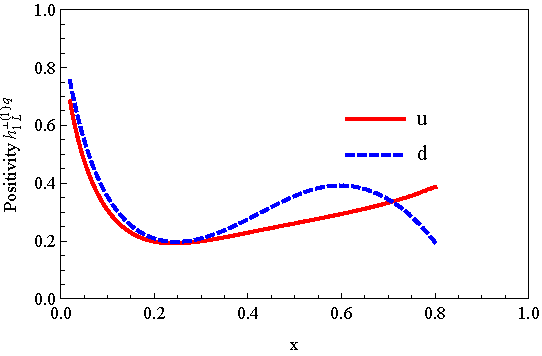
\includegraphics[width=0.45\textwidth]{\FigPath/h1lperp_positivity.pdf}  
	\caption{\label{h1l_pos} 
	LHS of Eq.~\eqref{eq:positivity1}.
}
\end{figure}
%%%%%%%%%%%%%%%%%%%%%%%%%%%%%%%%%%%%%%%%%%%%

%%%%%%%%%%%%%%%%%%%%%%%%%%%%%%%%%%%%%%%%%%%%%%%%%%%%%%%%%%%%%%%%%%%%%%%%%%%%%%%
\begin{figure}[h!]
\centering
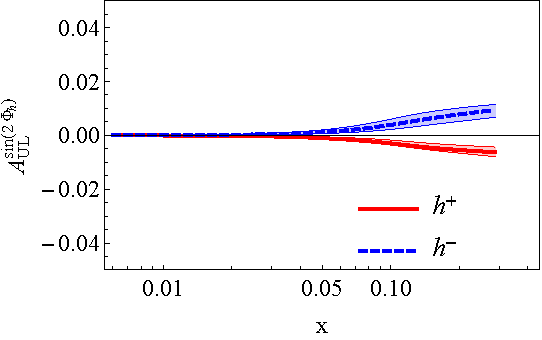
\includegraphics[width=0.45\textwidth]{\FigPath/AULsin2phi_COMPASS_x.pdf}  
	\caption{\label{aul_jlab} 
	$A_{UL}^{\sin(2\phi_h)}$  as a function of $ x $  at typical kinematics 
	of COMPASS, 
	$\la x\ra = 0.05$, $\la z\ra = 0.36$, $\la Q^2\ra = 2.4$ GeV$^2$.
	}
\end{figure}
%%%%%%%%%%%%%%%%%%%%
\newpage
%========= SECTION 8: TWIST-3 IN WW-TYPE APPROXIMATION ===============
\section{Subleading twist asymmetries in WW-type approximation}
\label{Sec-7:twist-3-and-WW}

The WW-type approximations are useful for all 8 subleading-twist observables,
as shown in Sec.~\ref{Sec-4.2:WW-twist-3}. In view of the complex 
structure of subleading-twist structure functions, WW-type approximations
might be particularly useful for the interpretation of twist-3 
observables. 

\subsection{\boldmath Subleading twist  $A_{LU}^{\sin\phi_h}$}
\label{Sec-7.1:FLU}

We start our discussion with the structure function $F_{LU}^{\sin\phi_h}$,
Eq.~(\ref{FLUsinphi}), containing 4 terms: 
2 are proportional to pure twist-3 fragmentation functions 
$\tilde{G}^{\perp a}$ and $\tilde{E}^a$ and neglected; the other 2
terms are proportional to the twist-3 TMDs $e^a$ and $g^{\perp a}$ which
also turn out to be given in terms of pure twist-3 terms upon the 
inspection of Eqs.~(\ref{Eq:WW-type-1},~\ref{Eq:WW-type-gperp}).
Hence, after consequently applying the WW-type approximation we are left 
with no term. Our approximation predicts this structure function to be zero.

Instead, data from Jefferson Lab and HERMES show a small but 
clearly non-zero effect of the order of (2-3)\,$\%$ 
\cite{Avakian:2003pk,Airapetian:2006rx,Gohn:2009zz,Aghasyan:2011ha,
Adolph:2014pwc,Gohn:2014zbz}.
What may seem at first glance to be a failure of the approach is in 
fact in line with it.
The important point is that in this case, the entire effect is due 
to $\bar qgq$-terms only. More precisely, the numerator of the 
asymmetry is proportional to $\bar q g q$-correlators, while the 
denominator is of course give by $f_1^aD_1^a$, i.e.\ in terms of
$q q$-correlators. Therefore we may formulate this approximation 
as follows
\be\label{Eq:ALU-small}
    A_{LU}^{\sin\phi_h}  
	\;\; \propto \;\;\frac{\la\bar qgq\ra}{\la\bar qq\ra}
    	\;\;\stackrel{\rm exp}{=} \;\; 
	{\cal O}\biggl( (2-3)\,\%\biggr)
    	\;.
\ee
We should keep in mind several reservations. First,
the experimental result quoted in (\ref{Eq:ALU-small})
contains also kinematic prefactors which help to reduce the value. 
Second, the denominator contains $f_1^a$ and $D_1^a$ which are the
largest TMD and FF because of positivity constraints. Third, the 
numerator is a sum of 4 terms, so its overall smallness could also 
result from cancellation of different terms, rather than indicating
that all 4 terms are small.
Keeping these reservations cautiously in mind, we may nevertheless 
consider the experimental observation of a (2-3)\,$\%$ asymmetry 
$A_{LU}^{\sin\phi_h}$ 
\cite{Avakian:2003pk,Airapetian:2006rx,Gohn:2009zz,Aghasyan:2011ha,
Adolph:2014pwc,Gohn:2014zbz}
as an encouraging indication that $\bar qgq$-terms are smaller than 
$\bar qq$ terms, in line with the generic expectation (\ref{Eq:WW-generic}).

To conclude, the WW-type approximation does not fail in the case of 
$F_{LU}^{\sin\phi}$. This is a unique observable, the only twist-3 SIDIS 
structure not ``contaminated'' by leading twist terms. 
Our WW-type approximation qualitatively predicts the asymmetry 
$A_{LU}^{\sin\phi}$ to be small which is in agreement with experiment.
It is beyond our approach to make in this case a quantitative prediction. 
We notice that one obtains a zero result for this asymmetry also in
the parton model motivated approach limited to leading twist TMDs 
\cite{Anselmino:2011ch}. 

\ \\
\blue{\bf
  COMPASS: https://arxiv.org/pdf/1401.6284.pdf \\
  data: https://hepdata.net/record/ins1278730}


\newpage
\subsection{\boldmath Subleading twist  $A_{LT}^{\cos\phi_S}$}
\label{Sec-7.2:FLTcosphiS}

In the WW-type approximation the structure function
$F_{LT}^{\cos\phi_S}$ is due to $g_T^a(x,\kperp)$ and $D_1^a(z,\pperp)$ 
whose collinear counterparts are more or less well known, see
Secs.~\ref{Sec-3.4:WW-classic-experiment} and \ref{Sec-5.1:FUU-basis}.

We assume the Gaussian Ansatz for $g_T^a(x,\kperp)$ 
\be
	g^{q}_{T}(x,\kperp^2) = 
	g^{q}_{T}(x)\,\frac{1}{\pi \avkperp_{g_{T}}}\,
	e^{-\kperp^2/{\avkperp_{g_{T}}}}\;,
	\label{eq:gtnew}
\ee
where $g^{q}_{T}(x)$ is calculated according to Eq.~\ref{Eq:WW-original1}.
Notice that we could have used WW-type relation of Eq.~(\ref{Eq:WW-type-6}) to relate $g^{q}_{T}(x,\kperp^2)$
and $g^{\perp q}_{1T}(x,\kperp^2)$ however we choose not to do it. In fact Eq.~(\ref{Eq:WW-type-6}) suggests kinematical zero 
$g^{q}_{T}(x, 0) = 0$  which is not supported by the model calculations \cite{Avakian:2010br} and thus  Eq.~(\ref{Eq:WW-type-6}) can be used only in its integrated form. 
The Eq.~(\ref{Eq:WW-type-6}) is not exact and is not on the same footing as WW-approximation of Eq.~(\ref{Eq:WW-original1}), and we parametrize directly $g^{q}_{T}(x,\kperp^2)$ using the Gaussian shape. For illustrative purpose we show ``violation'' of  Eq.~(\ref{Eq:WW-type-6}) in Fig.~\ref{altcosphi_wwtype}.


$F_{LT}^{\cos\phi_S}$
structure function then reads 
\begin{subequations}\ba
	F_{LT}^{\cos\phi_S}(x,z,\Phperp) 
	&=& -\frac{2M}{Q}\; x^2 \sum_q e_q^2\,g_T^q(x)\,D_1^q(z)\;   
	{ \cal G}(\Phperp)\, , \label{Eq:FLTcosphiS-Gauss}\\
	F_{LT}^{\cos\phi_S}(x,z)
	&=& -\frac{2M}{Q}\; x^2 \sum_q e_q^2\, g_T^q(x)\,D_1^q(z)\, ,
\ea\end{subequations}
with the width $\lambda= z^2 \avkperp_{g_T} + \avpperp_{D_1}$
in the Gaussian ${\cal G}(\Phperp)$. We estimate $g_T^a(x)$ in terms 
of $g_1^a(x)$ according to Eq.~(\ref{Eq:WW-original1}) assuming for 
the Gaussian width $\avkperp_{g_T}=\avkperp_{g_1}$.\footnote{
	Notice that one could also proceed in a different way: 
	explore first the WW-type-relation (\ref{Eq:WW-type-5}), and
	assume then the Gauss Ansatz for $g_{1T}^{\perp}(x,\kperp)$ 
	according to (\ref{eq:g1t}). Solving then the convolution integral 
	yields a result different from (\ref{Eq:FLTcosphiS-Gauss})
	which depends much more strongly on Gaussian model parameters.
	The operations of applying the WW-type approximations and 
	employing the Gauss Ansatz do not commute in general.
	The solution presented in (\ref{Eq:FLTcosphiS-Gauss}) is 
	preferable as it helps to minimize model dependence.}

Asymmetries $A_{LT}^{\cos\phi_S} = F_{LT}^{\cos\phi_S}/F_{UU}$ for 
COMPASS are plotted in Fig.~\ref{altcosphi_jlab}.
Notice that the asymmetry scales at small transverse hadron
momenta as $A_{LT}^{\cos\phi_S} \propto (\Phperp)^0$ which makes
it easier to measure if longitudinally polarized lepton beams
and transversely polarized targets are available.

\ \\
\PS{We should include a comparison to 
COMPASS data \cite{Kotzinian:2007uv,Parsamyan:2010se}.}


%%%%%%%%%%%%%%%%%%%%%%%%%%%%%%%%%%%%%%%%%%%%%%%%%%%%%%%%%%%%%%%%%%%%%%%%%%%%%%%
\begin{figure}[h!]
\centering
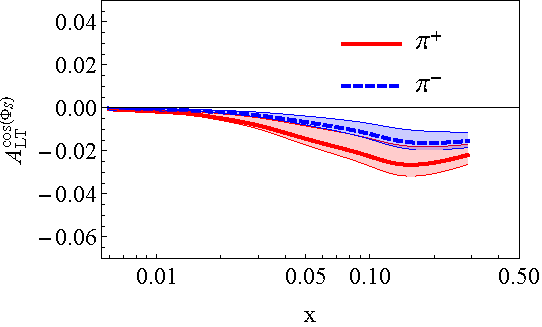
\includegraphics[width=0.45\textwidth]{\FigPath/ALTcosPhi_COMPASS_x.pdf} 
\caption{\label{altcosphi_jlab} $A_{LT}^{\cos\phi_S}$  as a function of $ x $.
}
\end{figure}
%%%%%%%%%%%%%%%%%%%%%%%%%%%%%%%%%%%%%%%%%%%%%%%%%%%%%%%%%%%%%%%%%%%%%%%%%%%%%%%

 %%%%%%%%%%%%%
\begin{figure}[h!]
\centering
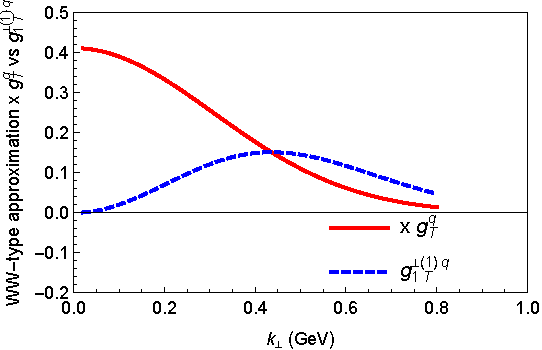
\includegraphics[width=0.45\textwidth]{\FigPath/gT_vs_g1Tperp_wwtype.pdf} 
\caption{\label{altcosphi_wwtype} RHS and LHS of Eq.~\ref{Eq:WW-type-6}.
}
\end{figure}
%%%%%%%%%%%%%%%%%%%%%%%%%%%%%%%%%%%%%%%%%%%%%%%%%%%%%%%%%%%%%%%%%%%%%%%%%%%%%%%



\newpage
\subsection{\boldmath   Subleading twist  $A_{LL}^{\cos\phi_h}$}
\label{Sec-7.3:FLLcosphi}

The structure function $F_{UL}^{\cos\phi_h}$ reads
\begin{subequations}\ba
	F_{LL}^{\cos \phi_h}(x,z,\Phperp)
	&=& -\,\frac{2M}{Q}\;x\sum_q e_q^2\,x\,g_{L}^{\perp (1) q}(x)\,D_1^{q}(z)\; 
	b^{(1)}_{\rm B}\,\biggl(\frac{z \Phperp} {\lambda}\biggr)\,
	{ \cal G}(\Phperp ) \, , \\ 
	F_{LL}^{\cos\phi_h}(x,z,\la\Phperp\ra) 
	&=& -\,\frac{2M}{Q}\;x\sum_q e_q^2\,x\,g_{L}^{\perp (1) q}(x)\,D_1^{q}(z)\;
	c^{(1)}_{\rm B}\,\biggl(\frac{z} {\lambda^{1/2}}\biggr)\, , 
\ea\end{subequations}
where $\lambda=z^2 \avkperp_{g_{L}^\perp} + \avpperp_{D_1}$, 
$b^{(1)}_{\rm B}=2M_N$,
$c^{(1)}_{\rm B} = \sqrt{\pi}\,M_N$, see App.~\ref{App:convol-details}.
We approximate the Gaussian width $\avkperp_{g_{L}^\perp}=\avkperp_{g_1}$ and 
estimate $g_L^{\perp(1) a}(x)$ according to Eq.~(\ref{Eq:WW-type-gLperp}) as
\be
	x\,g_L^{\perp(1) a}(x) = \frac{\la \kperp^2\ra_{g_1}}{2\,M_N^2}\,
	g_1^a(x) \,.
\ee
The asymmetries $A_{LL}^{\cos\phi_S}=F_{LL}^{\cos\phi_S}/F_{UU}$  for 
COMPASS are plotted in Fig.~\ref{allcosphi_jlab}.

\ \\
\PS{We should include a comparison to 
COMPASS data \cite{Kotzinian:2007uv,Parsamyan:2010se}.}

\



%%%%%%%%%%%%%%%%%%%%%%%%%%%%%%%%%%%%%%%%%%%%%%%%%%%%%%%%%%%%%%%%%%%%%%%%%%%%%%%
\begin{figure}[h!]
\centering
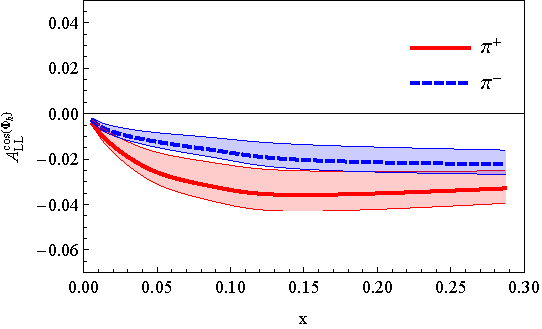
\includegraphics[width=0.45\textwidth]{\FigPath/ALLcosphi_COMPASS_x.pdf}  
	\caption{\label{allcosphi_jlab} 
	$A_{LL}^{\cos(\phi_h)}$  as a function of $ x $  at typical kinematics 
	of COMPASS, 
	$\la x\ra = 0.05$, $\la z\ra = 0.36$, $\la Q^2\ra = 2.4$ GeV$^2$.
	}
\end{figure}
%%%%%%%%%%%%%%%%%%%%

\newpage
\subsection{\boldmath Subleading twist $A_{UL}^{\sin\phi_h}$ }
\label{Sec-7.4:FULsinphi}

This twist-3 asymmetry has played a special role, as it was historically 
the first single spin asymmetry ever measured in SIDIS 
\cite{Airapetian:1999tv,Airapetian:2001eg,Airapetian:2002mf,Airapetian:2005jc}.
See also the recent COMPASS data \cite{Alekseev:2010dm}.
This asymmetry is sizable despite being twist-3. Although it was subject to 
numerous phenomenological studies, this asymmetry still remains unexplained.

Retaining the only non-zero term in the WW-type approximation, and
assuming for $h_L^q(x,\kperp)$ a Gaussian Ansatz 
\be
h_L^q(x,\kperp^2) = h_L^q(x) \,\frac{1}{\pi \avkperp_{h_{L}}}\,
	e^{-\kperp^2/{\avkperp_{h_{L}}}}\;,
	\label{eq:hLnew}
\ee
we obtain
for the structure function 
\begin{subequations}\ba
	F_{UL}^{\sin\phi_h}(x,z,\Phperp) 
	&=& \frac{2M}{Q}\,x\sum_q e_q^2\,x\,h_{L}^{q}(x)\,H_1^{\perp(1)q}(z)\; 
	b^{(1)}_{\rm A}\,\biggl(\frac{z \Phperp} {\lambda}\biggr)\,
	{ \cal G}(\Phperp ) \, , \\
	F_{UL}^{\sin\phi_h}(x,z,\la\Phperp\ra) 
	&=& \frac{2M}{Q}\,x\sum_q e_q^2\,x\,h_{L}^{q}(x)\,H_1^{\perp(1)q}(z)\;  
	c^{(1)}_{\rm A}\,\biggl(\frac{z} {\lambda^{1/2}}\biggr)\,
\ea\end{subequations}
where $\lambda=z^2 \avkperp_{h_L} + \avpperp_{H_1^\perp}$ and
$b^{(1)}_{\rm A}=2m_h$ and $c^{(1)}_{\rm A} = \sqrt{\pi}\,m_h$,
see App.~\ref{App:convol-details} for details. We now approximate 
$\avkperp_{h_L}=\avkperp_{h_1}$ and explore (\ref{Eq:WW-type-6}) to estimate
\be
	xh_L^q(x) = -2 h_{1L}^{\perp(1)q}(x)
\ee
and finally express $h_{1L}^{\perp(1)q}(x)$ in terms of $h_1^a(x)$
using (\ref{Eq:WW-approx-h1L}). $h_{1L}^{\perp(1)q}(x)$  is shown in Fig.~\ref{g1t_h1l_functions}.

The asymmetries $A_{UL}^{\sin\phi_h}=F_{UL}^{\sin\phi_h}/F_{UU}$  as a function of $x$  
for COMPASS is plotted in Fig.~\ref{aulsinphi_jlab} (a). We also compare our calculations to HERMES data \cite{Airapetian:2005jc} in Fig.~\ref{aulsinphi_jlab} (b).




%%%%%%%%%%%%%%%%%%%%%%%%%%%%%%%%%%%%%%%%%%%%%%%%%%%%%%%%%%%%%%%%%%%%%%%%%%%%%%%
\begin{figure}[ht]
\centering
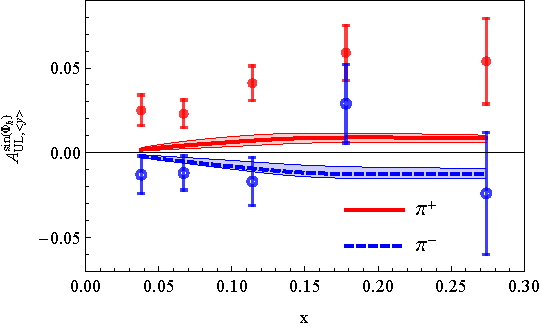
\includegraphics[width=0.45\textwidth]{\FigPath/AULsinphi_HERMES_x.pdf} (a)
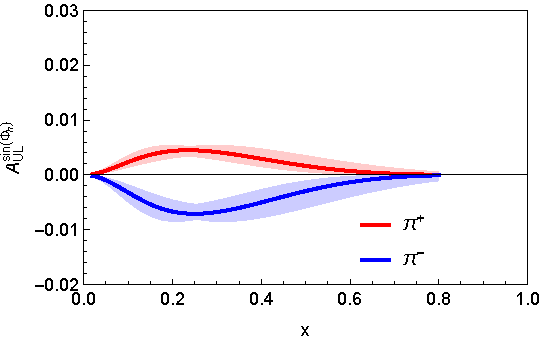
\includegraphics[width=0.45\textwidth]{\FigPath/AULsinphi_COMPASS_x.pdf} (b)
\caption{\label{aulsinphi_jlab} $A_{UL}^{\sin\phi_h}$  as a function of $ x $ , comparison to HERMES data \cite{Airapetian:2005jc} (a), and predictions for COMPASS (b).
}
\end{figure}
%%%%%%%%%%%%%%%%%%%%%%%%%%%%%%%%%%%%%%%%%%%%%%%%%%%%%%%%%%%%%%%%%%%%%%%%%%%%%%%


 

\newpage
\subsection{\boldmath Subleading twist  $A_{LT}^{\cos(2\phi_h - \phi_S)}$}
\label{Sec-7.5:FLTcos2phi-phiS}

Retaining the only non-zero term in the WW-type approximation, and
assuming for $g_T^{\perp a}(x,\kperp)$ a Gaussian Ansatz
\be
	g^{\perp q}_{T}(x,\kperp^2) = 
	g^{\perp (2) q}_{T}(x)\,\frac{2 M^4}{\pi \avkperp^3_{g_{T}^{\perp} }}\,
	e^{-\kperp^2/{\avkperp_{g_{T}^{\perp} }}}\;,
	\label{eq:gtperpnew}
\ee
We estimate $\avkperp_{g_{T}^\perp}=\avkperp_{g_1}$ and explore
the WW-type approximation (\ref{Eq:WW-type-gTperp}), 
\be
	xg_T^{\perp(2)q}(x) = \frac{\la\kperp^2\ra_{g_{1T}^\perp}}{M_N^2}\;
	g_{1T}^{\perp (1)q}(x)\,,
\ee
where we finally express $g_{1T}^{\perp (1)q}(x)$ in terms of $g_1^q(x)$ 
according to Eq.~(\ref{Eq:WW-approx-g1T}).

We obtain
for the structure function 
\begin{subequations}\ba
	F_{LT}^{\cos(2\phi_h - \phi_S)}(x,z,\Phperp) 
	&=& -\frac{2M}{Q} x \sum_q e_q^2\,x\,g_{T}^{\perp (2) q}(x)\,D_1^q(z)\; 
	b^{(2)}_{C}\,\biggl(\frac{z \Phperp} {\lambda}\biggr)^{\!2}\,
	{ \cal G}(\Phperp)\, , \\
	F_{LT}^{\cos(2\phi_h - \phi_S)}(x,z,\la\Phperp\ra) 
	&=& -\frac{2M}{Q} x \sum_q e_q^2\,x\,g_{T}^{\perp (2) q}(x)\,D_1^q(z)\;  
	c^{(2)}_{C}\,\biggl(\frac{z} {\lambda^{1/2}}\biggr)^{\!2}\,
	\label{eq:asymmetry_auu_cos2phi}
\ea\end{subequations}
where $\lambda=z^2 \avkperp_{g_{T}^\perp} + \avpperp_{D_1}$ and 
$b^{(2)}_{\rm C}=c^{(2)}_{\rm C} = M_N^2$, 
see App.~\ref{App:convol-details} for details. 


The asymmetry  $A_{LT}^{\cos(\phi_h -\phi_S)}=F_{LT}^{\cos(\phi_h -\phi_S)}/F_{UU}$ 
as a function of $x$ and $P_{hT}$ for COMPASS is plotted in 
Fig.~\ref{altcos2phi_jlab}.

\ \\
\PS{We should include a comparison to 
COMPASS data \cite{Kotzinian:2007uv,Parsamyan:2010se}.}

\

%%%%%%%%%%%%%%%%%%%%%%%%%%%%%%%%%%%%%%%%%%%%%%%%%%%%%%%%%%%%%%%%%%%%%%%%%%%%%%%
\begin{figure}[ht]
\centering
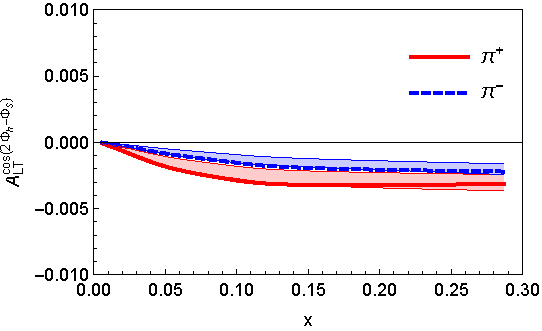
\includegraphics[width=0.45\textwidth]{\FigPath/ALTcos2PhiminusPhiS_COMPASS_x.pdf} 
\caption{\label{altcos2phi_jlab} $A_{LT}^{\cos(2\phi_h - \phi_S)}$  as a function of $ x $ for COMPASS.
}
\end{figure}
%%%%%%%%%%%%%%%%%%%%%%%%%%%%%%%%%%%%%%%%%%%%%%%%%%%%%%%%%%%%%%%%%%%%%%%%%%%%%%%


\newpage
\subsection{\boldmath Subleading twist  $A_{UT}^{\sin\phi_S}$}
\label{Sec-7.6:FUTsinphiS}

In the structure function $F_{UT}^{\sin\phi_S}$ we encounter 3 interesting 
new features. This is the first case with more than 1 contribution after 
applying the WW-type approximation. Assuming Gauss Ans\"atze for the TMDs
$f_T^q(x,\kperp)$, $h_T^{\perp q}(x,\kperp)$, $h_T^q(x,\kperp)$ 
we obtain 
\begin{subequations}\begin{alignat}{1}
	F_{UT}^{\sin\phi_S}(x,z,\Phperp) 
	&= \,\frac{2M}{Q}\;x\sum_q e_q^2\,\Biggl[
	  x\,f_T^q(x)
	\, D_1(z) \, { \cal G}(\Phperp)  \label{Eq:FUTsinphiS-Gauss-I-PhT}\\
	&- {\textstyle\frac12}\,x\,\left(h_T^{(1)q}(x)-h_T^{\perp(1)q}(x)\right)
	\,H_1^{\perp(1)q}(z)\; \frac{4z^2 m_h\,M_N}{\lambda} 
	\left(1-\frac{\Phperp^2}{\lambda}\right) {\cal G}(\Phperp) \Biggr] 
  	\nonumber\\
	F_{UT}^{\sin\phi_S}(x,z) 
	&= \,\frac{2M}{Q}\;x\sum_q e_q^2\, x\,f_T^q(x)\, D_1(z) 
	\label{Eq:FUTsinphiS-I-naive}\
\end{alignat}\end{subequations}
with  respectively
$\lambda=z^2\la\kperp^2\ra_{f_T}+\la\pperp^2\ra_{D_1}$ in the first, and  
$\lambda=z^2\la\kperp^2\ra_{h_T^\perp}+\la\pperp^2\ra_{H_1^\perp}$ in the 
second term of Eq.~(\ref{Eq:FUTsinphiS-Gauss-I-PhT}) where we 
assumed $\la\kperp^2\ra_{h_T^\perp}=\la\kperp^2\ra_{h_T^{ }}$. 

The second interesting feature not encountered before is that a contribution
drops out upon integrating the structure function over $\Phperp$, cf.\ 
Eq.~(\ref{Eq:FUTsinphiS-Gauss-I-PhT}) vs.\ (\ref{Eq:FUTsinphiS-I-naive}).
This is a property of the weight $\omega^{\{2\}}_{\rm B}$,
see Eq.~(\ref{Eq:wi}) and App.~\ref{App:factor}, which appears
also in $F_{LT}^{\cos\phi_S}$, Eq.~(\ref{FLTcosphiS}), where it however drops
out in WW-type approximation. In principle, this property could  help to 
discriminate experimentally the terms associated with this weight.

Exploring the WW-type approximations (\ref{Eq:WW-type-7},~\ref{Eq:WW-type-8}) 
the chiral odd twist-3 TMDs can be unambiguously related to transversity
\begin{subequations}\be
   	-\,{\textstyle\frac12}\,x \left(h_T^{(1)q}(x) - h_T^{\perp(1)q}(x)\right)
	= h_1^{(1)q}(x) = \frac{\la\kperp^2\ra_{h_1}}{2M_N^2}\,h_1^q(x)\, .
\ee
Now we encounter the third interesting feature, namely the treatment 
of $f_T^q(x)$ is not unambiguous. We could explore the sum rule 
(\ref{Eq:sum-rules-T-odd}) or employ the WW-type approximation 
(\ref{Eq:WW-type-fT}) to obtain 
\be
   	x \, f_T^q(x) 
	\stackrel{!?}{=} \begin{cases} 
	\phantom{-}\, 0 	
	& \mbox{due to sum rule (\ref{Eq:sum-rules-T-odd}),} \cr
	- \, f_{1T}^{\perp (1)q}(x) 
		& \mbox{due to WW-type (\ref{Eq:WW-type-fT}),} 
		\end{cases}\label{WW-type-fTperp-discuss-II}
		\;\;\;\;\;\;\;\;\;\;\;\;\;\;\;
\ee\end{subequations}
We recall that the twist-3 TMD $f_T^q(x,\kperp) \neq 0$ in general, 
but the collinear T-odd PDF $f_T^q(x) = 0$ due to time reversal, 
Eq.~(\ref{Eq:sum-rules-T-odd}). This was discussed in 
Sec.~\ref{Sec-3.7:basis+limitations}. 

Notice that in Eq.~(\ref{Eq:FUTsinphiS-Gauss-I-PhT}) we really have a 
choice, because we strictly speaking deal with the convoluted non-zero 
TMD $f_T^q(x,\kperp)$, and the Gauss model only {\it artificially} 
introduces the collinear function $f_T^q(x)$ expected to be zero.
However, in Eq.~(\ref{Eq:FUTsinphiS-I-naive}) we have no choice.
Here we really deal with the collinear function $f_T^q(x)$ which
must vanish due to the sum rule (\ref{Eq:sum-rules-T-odd}).
How should one proceed?

If we wish to respect the sum rule (\ref{Eq:sum-rules-T-odd}), 
we have to describe $f_T^q(x,\kperp)$ by a function with a node 
in $\kperp$. A simple Gaussian is not adequate for that. But from
phenomenological point of view, one of course could work with a 
superposition of Gaussians\footnote{
	The possibility of TMDs with nodes is not unrealistic.
	For instance in the covariant parton model the helicity TMDs 
	exhibit nodes for the $u$ and $d$- flavor \cite{Efremov:2010mt}.
	We will have to revise our description of $g_1^q(x,\kperp)$ 
	in Eq.~(\ref{eq:g1}) and App.~\ref{App:basis-g1} to something 
	of the type (\ref{Eq:multiple-Gauss}), if this prediction is 
	confirmed experimentally. }
with different widths, 
\begin{alignat}{1}
	x \, f_T^q(x,\kperp) =  - \, f_{1T}^{\perp (1)q}(x)\;
	&\sum\limits_{i=1}^{n} a_i\;
	\frac{\exp(-\kperp^2/\la\kperp^2\ra_i^{ }}{\pi\la\kperp^2\ra_i^{ }}\,,
	\nonumber\\
	&\sum\limits_{i=1}^n a_i = 0\,, \;\;
	\la\kperp^2\ra_i^{ }\neq\la\kperp^2\ra_j^{ }\;\;\forall\;i\neq j,
	\; 1\le i,\,j\le n,\;n\ge 2.\label{Eq:multiple-Gauss}
\end{alignat}
The minimal choice would be $n=2$ with $a_1=-a_2=1$ and
$\la\kperp^2\ra_1^{ } = \la\kperp^2\ra_{f_1^\perp}$ to make maximal use 
of the theoretical guidance provided by the WW-type approximation 
(\ref{Eq:WW-type-fT}). 
The second Gaussian width $\la\kperp^2\ra_2^{ }$ could then be chosen
very small $\la\kperp^2\ra_2^{ } \ll \la\kperp^2\ra_{f_1^\perp}$.
Within such a Gaussian description we would have a transverse momentum 
dependence of $f_T^{q}(x,\kperp^2)$ similar to that of 
$f_{1T}^{\perp(1)q}(x,\kperp^2)$ at not too small $\kperp$. 
A very small parameter $\la\kperp^2\ra_2^{ }$ could be thought of as 
a relict, e.g.\ of gluonic pole contributions in the $\bar qgq$-term 
$\tilde{f}_T^q(x,\kperp)$. It will be very interesting to follow up
on this in future studies.

At this point, however, we have no guidance from phenomenology or theory 
to fix additional parameters and choose a pragmatic and simple solution, 
namely to implement the sum rule (\ref{Eq:sum-rules-T-odd}) also in 
Eq.~(\ref{Eq:FUTsinphiS-Gauss-I-PhT}). This is
a model-dependent choice and this step could be revised along the
lines of the above discussion. Our final result is therefore
\begin{alignat}{1}
	F_{UT}^{\sin\phi_S}(x,z,\Phperp) 
	&= \,\frac{2M}{Q}\;x\sum_q e_q^2\,
	h_1^{(1)q}(x)\,H_1^{\perp(1)q}(z)\; \frac{4z^2 m_h\,M_N}{\lambda} 
	\left(1-\frac{\Phperp^2}{\lambda}\right) {\cal G}(\Phperp) 
	\nonumber\\
  	F_{UT}^{\sin\phi_S}(x,z) 
	&= 0 \, .	\label{Eq:FUTsinphiS-final}
\end{alignat}
In (\ref{Eq:FUTsinphiS-final}) we recover the consistent result for 
the ``collinear'' (i.e.\ related to the weight $\omega^{\{0\}}$) SIDIS 
structure function $F_{UT}^{\sin\phi_S}(x,z)$ in WW-type approximation, 
see Eq.~(\ref{Eq:FUT-collinear}). 

The asymmetries $A_{UT}^{\sin\phi_S}=F_{UT}^{\sin\phi_S}/F_{UU}$  for 
Jefferson Lab 12 GeV are plotted in Fig.~\ref{autsinphi_jlab}.
\PS{Compare to HERMES data \cite{Schnell:2010zza}?
Is there by now final data? Will be interesting!}


%%%%%%%%%%%%%%%%%%%%%%%%%%%%%%%%%%%%%%%%%%%%%%%%%%%%%%%%%%%%%%%%%%%%%%%%%%%%%%%
\begin{figure}[ht]
\centering
\includegraphics[width=0.45\textwidth]{\FigPath/AUTsinphi_x.pdf} 
\includegraphics[width=0.45\textwidth]{\FigPath/AUTsinphi_PT.pdf}
\caption{\label{autsinphi_jlab} $A_{UT}^{\sin\phi_S}$  as a function of $ x $ (left panel), and   as a function of $P_{hT}$ (right panel) at typical kinematics of Jefferson Lab 12 GeV, $\la x\ra = 0.25$, $\la z\ra = 0.54$, $\la Q^2\ra = 2.4$ GeV$^2$.
}
\end{figure}
%%%%%%%%%%%%%%%%%%%%%%%%%%%%%%%%%%%%%%%%%%%%%%%%%%%%%%%%%%%%%%%%%%%%%%%%%%%%%%%

 

\newpage
\subsection{\boldmath Subleading twist  $A_{UU}^{\cos\phi_h}$ }
\label{Sec-7.7:FUUcosphi}

Historically this was the first predicted \cite{Cahn:1978se} and measured
\cite{Aubert:1983cz} azimuthal asymmetry in (unpolarized) SIDIS, and
later explored in \cite{Anselmino:2005nn} to extract information on the 
Gaussian widths of $f_1^q(x,\kperp)$ and $D_1^q(x,\pperp)$ (under the 
implicit assumption of WW-type approximations).

The structure function $F_{UU}^{\cos\phi_h}$, Eq.~(\ref{Eq:FUUcosphi}),
contains after the WW-type approximation two contributions. Assuming
Gaussian Ans\"atze for $h^{q}(x,\kperp)$ and $f^\perp(x,\pperp)$ we obtain
\begin{subequations}\begin{alignat}{1}
	F_{UU}^{\cos\phi_h}(x,z,\Phperp) 
	= \red{+}\,\frac{2M}{Q}\;x\sum_q e_q^2\,\Biggl[
	  x\,h^{q}(x)\,H_1^{\perp(1)q}(z)\;b^{(1)}_{\rm A}\,
	  \biggl(\frac{z \Phperp} {\lambda}\biggr)\, & { \cal G}(\Phperp)
	  \nonumber\\
	\red{-} x\,f^{\perp(1)q}(x)\,D_1^q(z)\;b^{(1)}_{\rm B}\,
	  \biggl(\frac{z \Phperp} {\lambda}\biggr)\, & { \cal G}(\Phperp ) 
	\Biggr] \label{Eq:XXXa}\\
	F_{UU}^{\cos\phi_h}(x,z,\la\Phperp\ra) 
	= \red{+}\,\frac{2M}{Q}\;x\sum_q e_q^2\,\Biggl[
	  x\,h^{q}(x)\,H_1^{\perp(1)q}(z)\;c^{(1)}_{\rm A}\;
	  \biggl(\frac{z}{\lambda^{1/2}}\biggr)&
	  \nonumber\\
	\red{-}x\,f^{\perp(1)q}(x)\,D_1^q(z)\;c^{(1)}_{\rm B}\;
	  \biggl(\frac{z}{\lambda^{1/2}}\biggr)&
	\Biggr] \label{Eq:XXXb}
\end{alignat}\end{subequations}
with $\lambda=z^2\la\kperp^2\ra_{h}+\la\pperp^2\ra_{H_1^\perp}$ in the first, 
and  $\lambda=z^2\la\kperp^2\ra_{f^\perp}+\la\pperp^2\ra_{D_1}$ in the second 
term respectively in (\ref{Eq:XXXa}) and (\ref{Eq:XXXb}). The coefficients 
$b^{(1)}_i$ and $c^{(1)}_i$ are defined in App.~\ref{App:convol-details}.

The application of the WW-type approximation (\ref{Eq:WW-type-last}) 
for $h^q(x)$ is subtle. Applying it literally would imply 
$x\,h^q(x) = - 2\,h_1^{\perp(1)}(x)$ at variance with the sum rule
(\ref{Eq:sum-rules-T-odd}) for the collinear T-odd twist-3 TMD $h^q(x)$.
The situation is analog to the case of $f_T^q(x,\kperp)$
discussed in Sec.~\ref{Sec-7.6:FUTsinphiS}. Also here one could introduce
an additional Gauss parameter and use a double Gaussian to describe 
$h^q(x,\kperp)$. One should keep this in mind as an interesting possibility
to be explored in future studies. However, at this point we have no guidance
from theory or phenomenology to fix additional parameters. We therefore
proceed analogously to Sec.~\ref{Sec-7.7:FUUcosphi}, and impose 
(in a model-dependent step) the sum rule (\ref{Eq:sum-rules-T-odd}) 
by setting 
\begin{subequations}\be
	x\,h_1^q(x) = 0\,.
\ee

For $f^{\perp(1)}(x)$ we explore Eq.~(\ref{Eq:WW-type-Cahn}) as
\be
	x\,f^{\perp(1)}(x) = \frac{\la\kperp^2\ra_{f_1}}{2M_N^2}\,f_{1}^q(x)
	\, , 
\ee\end{subequations}
and estimate its Gaussian width as $\la\kperp^2\ra_{f^\perp}=\la\kperp^2\ra_{f_1}$.
The latter means the Gaussian factors of 
$F_{UU}^{\cos\phi_h}$ and $F_{UU}$ cancel out, i.e.\ at some point 
for $\Phperp\gtrsim1\,$GeV we would obtain from (\ref{Eq:XXXa}) 
an asymmetry $A_{UU}^{\cos\phi_h}=F_{UU}^{\cos\phi_h}/F_{UU}$ exceeding
100$\,\%$ and violating unitarity. This is of course an artifact of our 
approximations, and reminds us that the WW-type approximations as well
as the entire TMD formalism must be applied to small $\Phperp\ll Q$,
and in the case of $A_{UU}^{\cos\phi_h}$ preferably for $\Phperp < 1\,$GeV,
as shown in Fig.~\ref{auucosphi_jlab}. \\
\PS{(Alexei: did you notice it \cite{Anselmino:2005nn}? How did you treat it?)}

The asymmetries $A_{UU}^{\cos\phi_h}$  for 
Jefferson Lab 12 GeV are plotted in Fig.~\ref{auucosphi_jlab}.
\PS{We should compare to EMC, or 
	JLab \cite{Osipenko:2008aa,Mkrtchyan:2007sr}, 
	HERMES and COMPASS \cite{Giordano:2009hi,Joosten:2009zz}.
	There is probably also newer data!}





%%%%%%%%%%%%%%%%%%%%%%%%%%%%%%%%%%%%%%%%%%%%%%%%%%%%%%%%%%%%%%%%%%%%%%%%%%%%%%%
\begin{figure}[ht]
\centering
\includegraphics[width=0.45\textwidth]{\FigPath/AUUcosphi_x.pdf} 
\includegraphics[width=0.45\textwidth]{\FigPath/AUUcosphi_PT.pdf}
\caption{\label{auucosphi_jlab} $A_{UU}^{\cos\phi_h}$  as a function of $ x $ (left panel), and   as a function of $P_{hT}$ (right panel) at typical kinematics of Jefferson Lab 12 GeV, $\la x\ra = 0.25$, $\la z\ra = 0.54$, $\la Q^2\ra = 2.4$ GeV$^2$.
}
\end{figure}
%%%%%%%%%%%%%%%%%%%%%%%%%%%%%%%%%%%%%%%%%%%%%%%%%%%%%%%%%%%%%%%%%%%%%%%%%%%%%%%

\

\ \\
\PS{We may potentially run into positivity issues also for other observables. 
However, I would suggest not to worry too much. We see in the pictures that 
the respective asymmetries are smaller than 100$\,\%$ for reasonably small 
$\Phperp$ and can be happy with that! But perhaps we should include a 
comment somewhere?}


%------ BEGIN FIGURE 4: Phperp(z) AND Phperp^2(z) at HERMES ----------
        \begin{figure}[b!]
        \vspace{-0.6cm}
        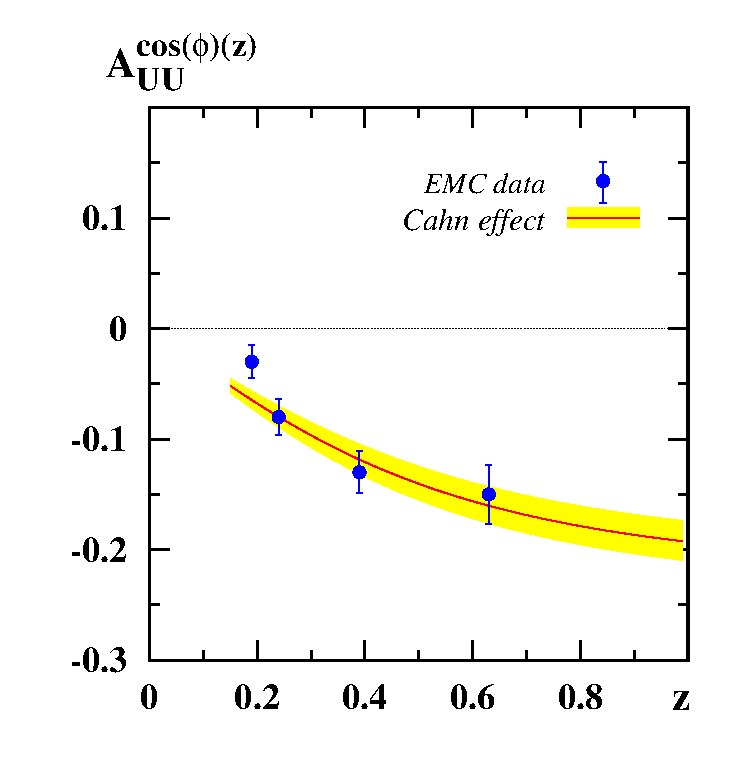
\includegraphics[height=8cm]{\FigPath/Fig06-EMC-cosphi-z.pdf}
        \vspace{-0.5cm}
        \caption{\label{Fig-02:EMC}
        Azimuthal asymmetry $A_{UU}^{\cos\phi}$ in charged hadron 
        production in SIDIS of $280\,{\rm GeV}$ muons off protons
        as function of $z$. The data from EMC \cite{Aubert:1983cz}
        refer to $\la Q\ra=4.8\,{\rm GeV}$. The theoretical
        curve is the ``WW-type and Cahn-effect-only'' approximation 
        for this observable in the Gauss model with parameters 
        fixed from HERMES data and neglecting evolution effects. 
	From Ref.~\cite{Schweitzer:2010tt}.}
        \end{figure}
%------ END FIGURE 4 -------------------------------------------------

\newpage
\subsection{\boldmath Subleading twist  $A_{UT}^{\sin(2\phi_h-\phi_S)}$ }
\label{Sec-7.8:FUTsin2phi-phiS}

In this last asymmetry we encounter the first case with more than 
1 contribution in our treatment. Assuming Gauss Ans\"atze for 
$f_T^{\perp q}(x,\kperp)$, $h_T^{\perp q}(x,\kperp)$, $h_T^q(x,\kperp)$ we find
\begin{subequations}\begin{alignat}{1}
	F_{UT}^{\sin(2\phi_h -\phi_S)}(x,z,\Phperp) \; \; 
	= \; \; \; \;
	\frac{2M}{Q}\;x\sum_q e_q^2\,\Biggl[
	x \; f_T^{\perp(2)q}(x) \; D_1(z) \;b^{(2)}_{\rm C}\;
	&\left(\frac{z\Phperp}{\lambda}\right)^{\!\!2}\;{ \cal G}(\Phperp) 
	\nonumber\\
	+ \;
	x\left(h_T^{(1)q}(x)+h_T^{\perp(1)q}(x)\right)H_1^{\perp(1)q}(z)\,
	\frac{b^{(2)}_{\rm AB}}{2}
	&\left(\frac{z\Phperp}{\lambda}\right)^{\!\!2}\;{\cal G}(\Phperp)\Biggr] 
	\label{Eq:FUTsin2phi-phiS-Gauss-PhT}\\
{ }
	F_{UT}^{\sin(2\phi_h -\phi_S)}(x,z,\Phperp) \; \; 
	= \; \; \; \;
	\frac{2M}{Q}\;x\sum_q e_q^2\,\Biggl[
	x \; f_T^{\perp(2)q}(x) \; D_1(z) \; c^{(2)}_{\rm C} \;
	&\biggl(\frac{z}{\lambda^{1/2}}\biggr)^{\!\!2}
	\nonumber\\
	+ \;
	x\left(h_T^{(1)q}(x)+h_T^{\perp(1)q}(x)\right)H_1^{\perp(1)q}(z)\,
	\frac{c^{(2)}_{\rm AB}}{2}
	&\biggl(\frac{z}{\lambda^{1/2}}\biggr)^{\!\!2}\Biggr] 
	\label{Eq:FUTsin2phi-phiS-Gauss}
\end{alignat}\end{subequations}
with respectively 
$\lambda=z^2\la\kperp^2\ra_{f_T^\perp}+\la\pperp^2\ra_{D_1}$ in the first, and  
$\lambda=z^2\la\kperp^2\ra_{h_T^\perp}+\la\pperp^2\ra_{H_1^\perp}$ in the second 
terms in 
Eqs.~(\ref{Eq:FUTsin2phi-phiS-Gauss-PhT},~\ref{Eq:FUTsin2phi-phiS-Gauss}).
We use $\la\kperp^2\ra_{h_T^\perp}=\la\kperp^2\ra_{h_T}$. The coefficients 
$b^{(2)}_i$ and $c^{(2)}_i$ are defined in App.~\ref{App:convol-details}.
We now explore the WW-type approximations in
Eqs.~(\ref{Eq:WW-type-fTperp},~\ref{Eq:WW-type-7},~\ref{Eq:WW-type-8}) to 
express the twist-3 TMDs in terms of the Sivers function and pretzelosity
as follows
\begin{subequations}\ba
   	x \, f_T^{\perp(2)q}(x) 
	&=& f_{1T}^{\perp (2)q}(x) 
	\equiv \frac{\la\kperp^2\ra_{f_{1T}^\perp}}{M_N^2}\,f_{1T}^{\perp (1)q}(x)\,,\\
   	-\,{\textstyle\frac12}\,x \left(h_T^{(1)q}(x) + h_T^{\perp(1)q}(x)\right)
	&=& h_{1T}^{\perp(2)q}(x) \, .
%	\equiv\frac{\la\kperp^2\ra_{f_{1T}^\perp}}{M_N^2}\,f_{1T}^{\perp(1)q}(x)
\ea\end{subequations}
%
%
% $xh_T^q(x,\kperp^2)        =-h_1^q(x,\kperp^2)-h_{1T}^{\perp(1)}(x,\kperp^2)$
% $xh_T^{\perp q}(x,\kperp^2)= h_1^q(x,\kperp^2)-h_{1T}^{\perp(1)}(x,\kperp^2)$
%
% $xf_T^{\perp q}(x,\kperp^2) = f_{1T}^{\perp   q}(x,\kperp^2)$
% $xf_T^{q}      (x,\kperp^2) =-f_{1T}^{\perp(1)q}(x,\kperp^2)$
%
% In our approach this is the only asymmetry which receives 2 contributions.
The asymmetries $A_{UT}^{\sin (2 \phi_h-\phi_S)}=F_{UT}^{\sin (2 \phi_h-\phi_S)}/F_{UU}$  
for Jefferson Lab 12 GeV are plotted in Fig.~\ref{autsin2phi_jlab}.

%%%%%%%%%%%%%%%%%%%%%%%%%%%%%%%%%%%%%%%%%%%%%%%%%%%%%%%%%%%%%%%%%%%%%%%%%%%%%%%
\begin{figure}[ht]
\centering
\includegraphics[width=0.45\textwidth]{\FigPath/AUTsin2phi_x.pdf} 
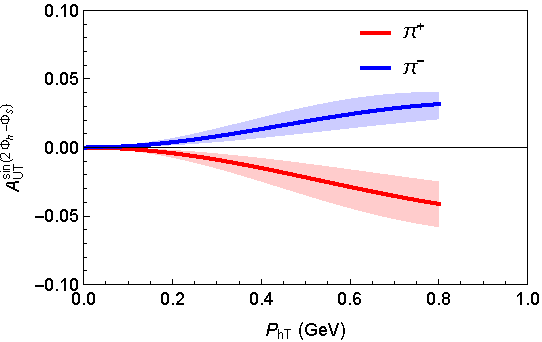
\includegraphics[width=0.45\textwidth]{\FigPath/AUTsin2phi_PT.pdf}
\caption{\label{autsin2phi_jlab} $A_{UT}^{\sin(2\phi_h- \phi_S)}$  as a function of $ x $ (left panel), and   as a function of $P_{hT}$ (right panel) at typical kinematics of Jefferson Lab 12 GeV, $\la x\ra = 0.25$, $\la z\ra = 0.54$, $\la Q^2\ra = 2.4$ GeV$^2$.
}
\end{figure}
%%%%%%%%%%%%%%%%%%%%%%%%%%%%%%%%%%%%%%%%%%%%%%%%%%%%%%%%%%%%%%%%%%%%%%%%%%%%%%%






{}

%======= SECTION 9: CONCLUSIONS ======================================
\newpage
\section{Conclusions  \judge{0$\,\%$ okay}}
\label{Sec-8:conclusions}

\red{\bf The following is just a collections of text fragments cut out
from the main text and pasted here in the hope it might be useful.}

\

% , and show that in this approximation all leading- and
% subleading-twist structure functions are expressed in terms of
% a ``basis'' consisting of 6 twist-2 TMDs and 2 twist-2 fragmentation 
% functions. 
It is important to remark that the generalized parton model 
approach of Ref.~\cite{Anselmino:2011ch} provides a description,
which is largely equivalent to ours.

\

The results presented in this work are of importance for several reasons.
First, to the best of our knowledge it is the first complete study 
of all SIDIS structure functions up to twist-3 in a unique approach. 
Second, the results are of use for experiments prepared in the near-term 
(Jefferson Lab 12) or proposed in the long-term (Electron Ion Collider),
and provide helpful input for Montecarlo event generators 
\cite{Avakian:2015vha}.
Third, our predictions will help to interpret data.
The quality of the approximations can only be determined experimentally. 
It is of importance to establish clear predictions, what we can expect 
to see in experiments on the basis of the WW approximation.
If our predictions will be confirmed, it will mean the WW-type approximations
for TMDs work well and call for theoretical explanations why.
If our predictions fail, it will mean that certain $\bar{q}gq$-terms are
sizable and call for theoretical studies to explain why.
In any case, we are going to learn important lessons


\

In the dedicated study \cite{Accardi:2009au} it was shown that the
error bars of the present data are compatible with a violation of the 
WW-approximation for $g_T^a(x)$ up to $40\,\%$ in certain regions of $x$. 
Rephrased in a more optimistic way, one may interpret the findings of
\cite{Accardi:2009au} as ``the WW approximation works to an accuracy of
 $40\,\%$ or better,'' and having an approximation with such a quality
for TMDs would be very valuable. It would help to interpret first
data, and allow us to make predictions for new experiments 
(JLab 12, EIC) where unknown TMDs contribute.

The aim of the presented study was to review what can be said about
the quality of  WW-(type-)approximations on the basis of results
from theory, models, and phenomenology. In particular, we have
presented a complete treatment of SIDIS observables in the
WW-type-approximation. This is what we found out.

Bla, bla, bla.



\section{Acknowledgments}
The authors would like to thank their families for the constant support during work on this project. This work was partially supported by the U.S.\
Department of Energy under Contract No.~DE-AC05-06OR23177 (A.P.) and by the National Science Foundation under Contract No. PHY-1623454 (A.P.).


 
\newpage
\appendix

\section{\boldmath The ``minimal basis" of TMDs and FFs}
\label{App:basis}

This Appendix describes the technical details of the parametrizations
used in this work.

\subsection{\boldmath Unpolarised functions $f_1^a(x,k_\perp)$ 
			and $D_1(z,P_\perp)$}
\label{App:basis-f1-D1}

In this work we use the leading-order parametrizations 
from \cite{Martin:2009iq} for the unpolarized PDF $f_1^a(x)$ and 
from \cite{deFlorian:2007aj} for the unpolarized FF $D_1^a(z)$.
If not otherwise stated the parametrizations are taken at the scale 
$Q^2=2.4\,{\rm GeV}^2$ typical for many currently available SIDIS data.
These parameterizations were used in \cite{Anselmino:2005nn} and other 
works whose extractions we adopt. 

To describe the transverse momentum dependence of $f_1^a(x,k_\perp)$ 
and $D_1(z,P_\perp)$ we use the Gaussian Ansatz in 
Eqs.~(\ref{Eq:Gauss-f1-D1}). All early 
\cite{Anselmino:2005nn,Collins:2005ie,D'Alesio:2007jt,Schweitzer:2010tt}
and some recent \cite{Signori:2013mda} analyses employed flavor and 
$x$- or $z$-independent widths $\avkperp$ and $\avpperp$.
In the the analysis \cite{Anselmino:2013lza} 
of HERMES multiplicities flavor-independence of the widths was 
assumed. On long run one may anticipate that new precision data will 
require to relax these assumptions. However, one may also expect that the 
Gaussian Ansatz will remain a useful {\it approximation} as long as one is 
interested in describing data on transverse hadron momenta $\Phperp \ll Q $. 

The parameters resulting from calculations or extractions are presented in
Table~\ref{Table:Gauss-paramaters}. 
As most extractions of TMDs that we will use are done with the choice of 
$\avkperp_{f_1} = 0.25$ GeV$^2$, $\avpperp_{D_1}= 0.2$ GeV$^2$, for our numerical estimates in this work  we will use these fixed widths.

Some comments are in order.
In \cite{Anselmino:2005nn} no attempt was made to assign an uncertainty of the 
best fit result. The uncertainty of the numbers from \cite{Schweitzer:2010tt}
includes only the statistical error, but no systematic uncertainty.
For comparison lattice results from \cite{Hagler:2009mb} are included
whose range indicates flavor-dependence 
(first number $u$-flavor,
second number $d$-flavor). 
Notice that this is the contribution of the flavor averaged
over contributions from the respective quarks and antiquarks.
Chiral theories predict significant differences in the $\kperp$-behavior
of sea and valence quarks \cite{Schweitzer:2012hh}.
We will comment more on the lattice results in the next section.
In view of the large (and partly underestimated) uncertainties and the 
fact that those parameters are anti-correlated the numbers from the 
different approaches quoted in Table~\ref{Table:Gauss-paramaters} 
can be considered to be in good agreement. 

\begin{table}[h!]
\centering
\begin{tabular}{|r|l|c|c|c|}
\hline
  & & & & \cr
  study \ \ \ \ 
	& $\;\;\la Q^2\ra$, $\la x\ra$, $\la z\ra$ 
	& $\avkperp_{f_1}$ 
  	& $\avpperp_{D_1}$ 
	& $\avkperp_{g_1}$ \cr
  	& {\footnotesize $[{\rm GeV}^2]$} 
  	& {\footnotesize $[{\rm GeV}^2]$} 
  	& {\footnotesize $[{\rm GeV}^2]$} 
  	& {\footnotesize $[{\rm GeV}^2]$} \cr
  & & & & \cr
\hline
  & & & & \cr
\ fit of \cite{Anselmino:2005nn} & 5, 0.1, 0.3
	& $\sim 0.25$ 
	& $\sim 0.2$ 
	& -- \cr
\ fit of \cite{Schweitzer:2010tt} & 2.5, 0.1, 0.4 
	& $0.38\pm0.06$ 
	& $0.16\pm0.01$ 
	& -- \cr
\ fit of \cite{Anselmino:2013lza} & 2.4, 0.1, 0.3 
	& $0.57\pm0.08$ 
	& $0.12\pm0.01$ 
	& -- \cr
\ fit of \cite{Signori:2013mda} & 2.4, 0.1, 0.5 
	& $\sim0.3$
	& $\sim0.18$ 
	& -- \cr
\ lattice \cite{Hagler:2009mb}  & 4, -- , --
	& 0.14--0.15   
	& -- 
	& 0.11-0.15 \cr
  & & & & \cr 
\hline
\end{tabular}
\caption{\label{Table:Gauss-paramaters}
  	Gauss model parameters for $f_1^a(x,k_\perp)$, $D_1^a(z,P_\perp)$, 
 	$g_{1}^a(x,k_\perp)$ from phenomenological and lattice QCD studies.
  	The kinematics to which the phenomenological results and the
	renormalization scale of the lattice results are indicated.
	The range of lattice values indicates flavor dependence
        (first number refers to $u$-flavor, second number to $d$-flavor).}
\end{table}


\subsection{\boldmath Helicity distribution $g_1^a(x,k_\perp)$}
\label{App:basis-g1}

For the helicity PDF $g_1^a(x)=\int d^2k_\perp\,g_1^a(x,k_\perp)\equiv 
\int d^2k_\perp\,g_{1L}^a(x,k_\perp)$ we use in this work the leading-order 
parameterizations from \cite{Gluck:1998xa}.
If not otherwise stated the parametrizations are taken at the scale 
$Q^2=2.5\,{\rm GeV}^2$.

In lack of phenomenological information on the $k_\perp$-dependence of
$g_1^a(x,k_\perp)$ we explore lattice QCD results from \cite{Hagler:2009mb}
to constrain the Gaussian width in Eq.~(\ref{eq:g1}). 
On a lattice with pion and nucleon masses 
$m_\pi\approx 500\,{\rm MeV}$ and $M_N=1.291(23)\,{\rm GeV}$ 
and with an axial coupling constant $g_A^{(3)}= 1.209(36)$ reasonably
close to its physical value $1.2695(29)$ the following results were
obtained for the mean square transverse parton momenta \cite{Hagler:2009mb}.
For the unpolarized TMDs it was found
$\langle \kperp^2 \rangle_{f_1^u} = (0.3741\,{\rm GeV})^2$ and
$\langle \kperp^2 \rangle_{f_1^d} = (0.3839\,{\rm GeV})^2$.
For the helicity TMDs it was found
$\avkperp_{g_1^u} = (0.327\,{\rm GeV})^2$ and
$\avkperp_{g_1^d} = (0.385\,{\rm GeV})^2$. 
These values are quoted in Table~\ref{Table:Gauss-paramaters}.

The lattice values for $\langle \kperp^2 \rangle_{f_1}$ consistently 
underestimate the phenomenological numbers, see 
Table~\ref{Table:Gauss-paramaters}.
The exact reasons for that are unknown, but it is natural to think it
might be related to the fact that the lattice predictions \cite{Hagler:2009mb}
do not refer to TMDs entering in SIDIS (or Drell-Yan or other process) 
because a different gauge link was chosen, see Sec.~\ref{Sec-3.5:WW-lattice}. 
Still one may expect these results to bear considerable information 
on QCD dynamics.\footnote{
	The results \cite{Hagler:2009mb} refer also to pion masses above the 
	physical value. This is caveat is presumably less critical and
	will be overcome as lattice QCD simulations are becoming feasible 
	at physical pion masses.}
To make use of this information we shall assume that the lattice results
\cite{Hagler:2009mb} provide robust predictions for the {\it ratios}
$\langle \kperp^2 \rangle_{g_1^u}/\langle \kperp^2 \rangle_{f_1^u}\approx 0.76$.
With the phenomenological value $\langle \kperp^2 \rangle_{f_1} = 0.25$ GeV$^2$ 
we then obtain the estimate for the width of the helicity TMD
$\langle \kperp^2 \rangle_{g_1} = 0.19$ GeV$^2$.
In our phenomenological study we use this value for $u$-quarks and for 
simplicity also for $d$-quarks. Even though the lattice values indicate 
an interesting flavor dependence, see Table~\ref{Table:Gauss-paramaters},
for a proton target this is a very good approximation due to $u$-quark 
dominance. When precision data for deuterium and especially for $^3$He
from Jefferson Lab become available, it will be interesting to 
re-investigate this point in detail.

\subsection{\boldmath Sivers function $f_{1T}^{\perp q}(x,k_\perp)$}
\label{App:basis-f1Tperp}

Sivers distribution function was studied in Refs.~\cite{Efremov:2004tp,Anselmino:2008sga,Anselmino:2011gs,Anselmino:2011ch, Aybat:2011ge,Gamberg:2013kla,Bacchetta:2011gx,Anselmino:2012aa,Sun:2013dya,Echevarria:2014xaa}. 
We will use parametrizations from  Refs.~\cite{Anselmino:2008sga,Anselmino:2011gs,Anselmino:2011ch}:
\ba
 \avkperp_{f_{1T}^\perp} &\equiv& \frac{\avkperp M_1^2}{\avkperp + M_1^2} \\
f_{1T}^{\perp}(x, \kperp^2)& =& - \frac {M}{M_1} \sqrt{2e} \;
{\cal N}_q(x) \, f_{q/p} (x,Q) \, \frac{e^{-\kperp^2/{\avkperp_{f_{1T}^\perp}}}}{\pi \avkperp} ,
\label{fiTp}
\ea
%
where $M_1$ is a mass parameter, $M$ the proton mass and
%
\ba
{\cal N}_q(x)= N_q \, x^{\alpha} (1-x)^{\beta} \,
\frac{(\alpha + \beta)^{(\alpha +\beta)}}
{\alpha^{\alpha} \beta^{\beta}}
 \ea
The first moment of Sivers function is:
\ba
f_{1T}^{\perp (1) q}(x)  = -\frac{\sqrt{\frac{e}{2}} \ \avkperp M_1^3}{M (\avkperp + M_1^2)^2}  \ {\cal N}_q(x)  f_q(x, Q) = -\sqrt{\frac{e}{2}} \frac{1}{M M_1}  \frac{\avkperp_{f_{1T}^\perp}^2}{\avkperp}    \ {\cal N}_q(x)  f_q(x, Q)
\label{siversm} \ .
\ea

We can rewrite parameterizations of Sivers functions as

\ba
f_{1T}^{\perp q}(x,\kperp) =  f_{1T}^{\perp (1) q}(x)   \frac{2 M^2}{\pi \avkperp_{f_{1T}^\perp}^2} e^{-\kperp^2/{\avkperp_{f_{1T}^\perp}}}
\label{sivers_new} \ .
\ea

The fit the HERMES proton and COMPASS deuteron data from 
including only Sivers functions for $u$ and $d$ quarks was done in Ref.~\cite{Anselmino:2011gs},
corresponding to seven free parameters, and parameters are shown in Table~\ref{tab:a}.


\begin{table}
\centering
\begin{tabular}{ccc}
\hline
$N_u=0.40$ & $\alpha_u=0.35$ & $\beta_u=2.6$ \\
$N_d=-0.97$ & $\alpha_d=0.44$ & $\beta_d=0.90$\\
& $M_1^2=0.19\textrm{(GeV}^2$) &   \\
\hline
\end{tabular}
\caption{Best values of the fit of the Sivers functions. Table from Ref.~\cite{Anselmino:2011gs}}
\label{tab:a}
\end{table}



\subsection{\boldmath Transversity $h_{1}^{q}(x,k_\perp)$ and 
Collins function $H_{1}^{\perp q}(x,P_\perp)$}
\label{App:basis-h1-H1perp}

These functions were studied in  
Refs.~\cite{Anselmino:2007fs,Anselmino:2008jk,Anselmino:2013vqa,
Kang:2014zza,Kang:2015msa,Anselmino:2015sxa}.
The following shape was assumed for parametrizations 
Refs.~\cite{Anselmino:2007fs,Anselmino:2008jk,Anselmino:2013vqa}:
 \ba
h_{1}^{q} (x, \kperp^2) &=&h_{1}^{q} (x)  \frac{e^{-{\kperp^2}/{\avkperp_{h_1} }}}{\pi \avkperp_{h_1}} \; ,\label{tr-funct}\\
h_{1}^{q} (x) &=&\frac{1}{2} {\cal N}^{\T}_q(x)\,
[f_{1}(x)+g_1(x)]\; ,\\
H_{1 h/q}^{\perp}(z, \pperp^2) = \frac{z m_h}{2 \pperp} \Delta^N \! D_{h/q^\uparrow}(z,\pperp^2) &=&  \frac{z m_h}{M_C} e^{-p_{\perp}^2/M_C^2} \sqrt{2 e} H_{1 h/q}^{\perp}(z) \,\frac{e^{-\pperp^2/{\avpperp}}}{\pi \avpperp}\,,
\label{coll-funct}
 \ea
 with $m_h$ produced hadron mass and
 \ba
 {\cal N}^{\T}_q(x)= N^{\T}_q
\,x^{\alpha} (1-x)^{\beta} \, \frac{(\alpha + \beta)^{(\alpha
+\beta)}} {\alpha^{\alpha} \beta^{\beta}}\; ,
\\
H_{1 h/q}^{\perp}(z) =  {\cal N}^{\C}_q(z) D_{h/q}(z)\, , \\
{\cal N}^{\C}_q(z)= N^{\C}_q \, z^{\gamma} (1-z)^{\delta} \,
\frac{(\gamma + \delta)^{(\gamma +\delta)}}
{\gamma^{\gamma} \delta^{\delta}}\, ,
 \ea
and $-1\le N^{\T}_q\le 1$, $-1 \le N^{\C}_q \le 1$. The helicity distributions $g_1(x)$ are taken
from Ref.~\cite{Gluck:2000dy}, parton distribution and fragmentation functions are the GRV98LO PDF set~\cite{Gluck:1998xa} and the
DSS fragmentation function set~\cite{deFlorian:2007aj}. Notice that with these choices both
the transversity and the Collins function automatically obey their
proper positivity bounds. Note that as in Ref.~\cite{Anselmino:2013vqa} we use two 
Collins fragmentation functions, {\it favored} and {\it disfavored} ones, see Ref.~\cite{Anselmino:2013vqa} for details on implementation, and corresponding parameters ${N}^{\C}_a$ are then  ${N}^{\C}_{fav}$ and ${N}^{\C}_{dis}$. For numerical estimates we use parameters extracted in Ref.~\cite{Anselmino:2013vqa}, see Table~\ref{fitpar}.

\begin{table}[h]
\centering
\renewcommand{\tabcolsep}{0.4pc} % enlarge column spacing
\renewcommand{\arraystretch}{1.2} % enlarge line spacing
\begin{tabular}{@{ }ll}
 \hline
 $N_{u}^{\T}$ = $0.46^{+0.20}_{-0.14}$ & $N_{d}^{\T}$ = $ -1.00^{+1.17}_{-0.00}$ \\
 $\alpha$ =  $1.11^{+0.89}_{-0.66}$ & $\beta$  = $3.64^{+5.80}_{-3.37}$ \\
 $\avkperp_{h_1} = 0.25$ (GeV$^2$) & \\
 \hline
 $N_{\rm fav}^{\C}$  = $0.49^{+0.20}_{-0.18}$ & $N_{\rm dis}^{\C}$  = 
 $-1.00^{+0.38}_{-0.00}$ \\
 $\gamma$  = $1.06^{+0.45}_{-0.32}$  & $\delta$   = $0.07^{+0.42}_{-0.07}$    \\
 $M^2_C = 1.50^{+2.00}_{-1.12}$ (GeV$^2$) & \\
 \hline
\end{tabular}
\caption{
Best values of the 9 free parameters fixing the $u$ and $d$ quark
transversity distribution functions and the favored and
disfavored Collins fragmentation functions. The table is from Ref.~\cite{Anselmino:2013vqa}.
\label{fitpar}}
\end{table}


According to Eq.~(\ref{eq:moments}) we obtain the following expression for the first moment of 
Collins fragmentation function: 
\ba
H_{1 h/q}^{\perp (1)}(z) = \frac{H_{1 h/q}^{\perp}(z) \sqrt{e/2}  \avpperp M_C^3}{z m_h  (M_C^2+\avpperp)^2}\; .
\ea 
We also define the following variable:
\ba
\avpperp_{H_1^\perp} = \frac{\avpperp M_C^2 }{\avpperp + M_C^2} .  
\ea

We can rewrite the parameterizations of Collins FF as

\ba
H_{1}^{\perp}(z,\pperp) =  H_{1}^{\perp (1)}(z)   \frac{2 z^2 m_h^2}{\pi \avpperp_{H_{1}^\perp}^2} e^{-\pperp^2/{\avpperp_{H_{1}^\perp}}}
\label{coll-funct_new} \, .
\ea

\subsection{\boldmath Boer-Mulders function $h_{1}^{\perp}(x,k_\perp)$} 
\label{App:basis-h1perp}

The Boer-Mulders function $h_{1}^{\perp}$~\cite{Boer:1997nt} measures 
the transverse polarization asymmetry of quarks inside an unpolarized 
nucleon. The Boer-Mulders functions were studied phenomenologically in 
Refs.~\cite{Barone:2009hw,Barone:2010gk,Barone:2015ksa}

The following parameterization was used in Refs.~\cite{Barone:2015ksa}:
\ba
\avkperp_{h_1^\perp} &=& \frac{\avkperp \, M^2_{BM}}{\avkperp + M^2_{BM}} \, , \\
h_{1}^{\perp}(x, \kperp^2) &= &
- \,\frac{M}{M_{BM}}  
\sqrt{2e}\; N_q 
\, f_{q/p} (x, Q)\frac{e^{-\kperp^2/\avkperp_{h_{1}^{\perp}}}}{\pi\avkperp},  
\label{BM-dist}
\ea
 
The first moment of Boer-Mulders function is:
\ba
h_{1}^{\perp (1) q}(x)  = -\frac{\sqrt{\frac{e}{2}} \ \avkperp M_{BM}^3}{M (\avkperp + M_{BM}^2)^2}  \ {N}_q f_q(x, Q) = -\sqrt{\frac{e}{2}} \frac{1}{M M_{BM}}  \frac{\avkperp_{h_1^\perp}^2}{\avkperp}    \ {N}_q  f_q(x, Q)
\label{bm} \ .
\ea
 
We can rewrite parameterization of Boer-Mulders functions as

\ba
h_{1}^{\perp q}(x,\kperp) =  h_{1}^{\perp (1) q}(x)   \frac{2 M^2}{\pi \avkperp_{h_{1}^\perp}^2} e^{-\kperp^2/{\avkperp_{h_{1}^\perp}}}\label{bm_new} \ .
\ea
 
 
%
\begin{table}[htb]
\centering
\begin{tabular}{l c l l c l}
\hline
 $N_{u}$ &=& $-0.49 \pm 0.15$ & $N_{d}$ &=& $-1 \pm 0.2$\\
 $M_{BM}^2$ &=& $0.1 \pm  0.2$&\multicolumn{3}{l}{(GeV$^2$)}\\ 
\hline
\end{tabular}
\caption{Fitted parameters of Boer-Mulders quark distributions. Values are from Ref.~\cite{Barone:2015ksa}}
\label{fitparbm}
\end{table}
 
\subsection{\boldmath Pretzelosity distribution $h_{1T}^{\perp}(x,k_\perp)$}
\label{App:basis-h1Tperp}

Pretzelosity   distribution function   
$h_{1T}^{\perp}$~\cite{Lefky:2014eia} describes transversely polarized quarks 
inside a transversely polarized nucleon.
We use the following form of $h_{1T}^{\perp a}$ ~\cite{Lefky:2014eia}:
\ba
h_{1T}^{\perp a}(x,k_{\perp}^2) = \frac{M^2}{M_{TT}^2} e^{-\kperp^2/M_{TT}^2} h^{\perp a}_{1T}(x) \frac{e^{-{\kperp^2}/{\avkperp}}}{\pi \avkperp}=\frac{M^2}{M_T^2} h^{\perp a}_{1T}(x) \frac{e^{-{\kperp^2}/{\avkperp_{h_{1T}^\perp}}}}{\pi \avkperp}\,\;,
\label{eq:h1Tperp}
\ea
where
\ba
h^{\perp a}_{1T}(x) = e  \ {\cal N}^a(x) (f_{1}^{a}(x, Q) - g_{1}^{a}(x, Q)), \label{eq:hx_par}\\
{\cal N}^a(x) = N^{a} x^{\alpha} (1-x)^{\beta} \frac{(\alpha + \beta)^{\alpha + \beta}}{\alpha^{\alpha} \beta^{\beta}}\, ,  \\
\avkperp_{h_{1T}^\perp}  = \frac{\avkperp M_{TT}^2}{\avkperp + M_{TT}^2}\, ,
\ea
where ${N}^a$, $\alpha$, $\beta$, and $M_T$ are parameters fitted to data that can be found in Table~\ref{fitparI}.

  We use Eq.~(\ref{eq:moments}) to calculate the second moment of $ h_{1T}^{\perp a}(x,\kperp^2)$
of Eq.~(\ref{eq:h1Tperp}) and obtain:
\be
h_{1T}^{\perp (2) a}(x) =  \frac{h^{\perp a}_{1T}(x) \avkperp_{h_{1T}^\perp}^3}{2 M^2 M_{TT}^2 \avkperp} \, .
\ee

We can rewrite parametrization of pretzelosity   functions as

\ba
h_{1T}^{\perp q}(x,\kperp) =  h_{1T}^{\perp (2) q}(x)   \frac{2 M^4}{\pi \avkperp_{h_{1T}^\perp}^3} e^{-\kperp^2/{\avkperp_{h_{1T}^\perp}}}
\label{pretzelosity_new} \ .
\ea

%
\begin{table}[htb]
\centering
\begin{tabular}{l c l l c l}
\hline
$\alpha$ &=& $2.5\pm1.5$ & $\beta$ &=& $2$ fixed \\
 $N_{u}$ &=& $1 \pm 1.4$ & $N_{d}$ &=& $-1 \pm 1.3$\\
 $M_{TT}^2$ &=& $0.18 \pm  0.7$&\multicolumn{3}{l}{(GeV$^2$)}\\ 
\hline
\end{tabular}
\caption{Fitted parameters of the pretzelosity quark distributions. Table from Ref.~\cite{Lefky:2014eia}}
\label{fitparI}
\end{table}
%
 
\newpage
\section{Convolution integrals and expressions in Gaussian Ansatz}}
\label{App:factor}

In this Appendix we explain the notation for convolution integrals
of TMDs and FFs and give the explicit results obtained assuming the
Gaussian Ansatz.

\subsection{Notation for convolution integrals \label{ApendixB1}}
 
Structure functions are expressed as convolutions of TMDs and FFs 
in the Bjorken limit at tree level. For reference we quote the 
convolution integrals in ``Amsterdam notation'' \cite{Bacchetta:2006tn}
\be
	{\cal C}\bigl[ w\slim f\slim D \bigr]
	=  x \, \sum_a e_a^2 \int d^2 {\bm p}_T \,  d^2 {\bm k}_T
	\, \delta^{(2)}\bigl({\bm p}_T - {\bm k}_T - {\bm P}_{h \perp}/z \bigr)
	\,w({\bm p}_T,{\bm k}_T)\,
	f^a( x ,p_T^2)\,D^a(z,z^2 k_T^2) , \label{eq:convolution-Amsterdam}
\ee
where all transverse momenta refer to the virtual photon-proton 
center-of-mass frame and $\bfhp  ={\bm P}_{h \perp}/{P}_{h\perp}$. 
Hereby ${\bm p}_T$ is 
the transverse momentum of quark with respect to nucleon, 
${\bm k}_T$ is the transverse momentum of the fragmenting quark 
with respect to produced hadron. The notation is not unique. 
The one chosen in this work, in comparison to other works, is 
\begin{alignat}{3} 
	\mbox{transverse momentum in TMD:}\;\;\;&
    	\left[\bfkperp\right]_{\rm our}
    &=& 	\left[{\bm k}_\perp\right]_{\mbox{\tiny Ref.\cite{Anselmino:2011ch}}} \;
    =  	\;\;\;\;\;\left[{\bm p}_T\right]_{\mbox{\tiny Ref.\cite{Bacchetta:2006tn}}}\,,
	\\
	\mbox{transverse momentum in \ FF:}\;\;\;&
	\left[\bfpperp\right]_{\rm our}
    &=& 	\left[{\bm p}_\perp\right]_{\mbox{\tiny Ref.\cite{Anselmino:2011ch}}} \;
    =  	-z\left[{\bm k}_T\right]_{\mbox{\tiny Ref.\cite{Bacchetta:2006tn}}}\,, 
	\\
	\mbox{transverse hadron momenta:}\;\;\;&
    	\left[\bfPhperp\right]_{\rm our}
    &=&	\left[{\bm P}_T\right]_{\mbox{\tiny Ref.\cite{Anselmino:2011ch}}} \;
    =  	\;\;\;\left[{\bm P}_{h\perp}\right]_{\mbox{\tiny Ref.\cite{Bacchetta:2006tn}}}\,.
\end{alignat}
Notice that 
$\left[\bfpperp\right]_{\rm our}=
-z\left[{\bm k}_T\right]_{\mbox{\tiny Ref.\cite{Bacchetta:2006tn}}}$ 
is the transverse momentum the hadron acquires in the fragmentation process.
The normalization for unpolarized fragmentation functions is 
\be
	D_1^a(z) 
	= \left[\,\int d^2{\bm P}_\perp D_1^a(z,P_\perp^2)\right]_{\rm our}
	= \left[z^2\int d^2{\bm k}_TD_1^a(z, z^2  k_T^2)
	  \right]_{\mbox{\tiny Ref.~\cite{Bacchetta:2006tn}}}
	\label{eq:D1}\;. 
\ee
The ``Amsterdam'' convolution integral (\ref{eq:convolution-Amsterdam})
reads in our notation
\be
	{\cal C}\bigl[ w\slim f\slim D \bigr]
	=  x \,
	\sum_a e_a^2 \int d^2 \bfkperp\,  d^2 \bfpperp^{ }
	\, \delta^{(2)}\bigl(z\bfkperp + \bfpperp - \bfPhperp \bigr)
	\,w\left(\bfkperp,-\frac{\bfpperp^{ }}{z}\right)
	f^a( x ,\kperp^2)\,D^a(z,\pperp^2) . \label{eq:convolution_our}
\ee

\subsection{Gaussian Ansatz}

For a generic TMD and FF the Gaussian Ansatz is given by 
\be
    f^a(x,\kperp^2)=
    f^a(x)\,\frac{\exp(-\kperp^2/\la\kperp^2\ra)}{\pi\la\kperp^2\ra}\,,\;\;\;
    D^a(z,\pperp^2)=
    D^a(z)\,\frac{\exp(-\pperp^2/\la\pperp^2\ra)}{\pi\la\pperp^2\ra}
\ee
where 
$\la\kperp^2\ra$ could be $x$-dependent,  
and $\la\pperp^2\ra$ $z$-dependent. 
Both could be flavor-dependent.
The variable $\pperp$ is convenient because phenomenological experience 
shows that $\pperp$ in $D_1^{q/h}(z,\pperp^2)$ exhibits a Gaussian distribution 
with weakly $z$-dependent Gaussian width. The distribution of transverse 
momenta in $\left[D^a(z,z^2 k_T^2)\right]_{\mbox{\tiny Ref.\cite{Bacchetta:2006tn}}}$ 
would require a strongly $z$-dependent Gaussian width. It is of course 
a matter of taste which one prefers to use.

It is convenient to work with transverse moments of TMDs and FFs
which are defined, and in the Gaussian model given by
\begin{alignat}{6}
	f^{(n)}(x) &=& \int d^2\bfkperp
	\left(\frac{\kperp^2}{2M^2}\right)^{\!\!n}\; f(x, \kperp^2)
	\;&\stackrel{\rm Gauss}{=}&\;
	\frac{n!\,\la \kperp^2\ra^n}{ 2^n\,M_N^{2n}}\, f(x),\;\;\;\nonumber\\
	D^{(n)}(z) &=& \int d^2\bfpperp
	\left(\frac{\pperp^2}{2 z^2 m_h^2}\right)^{\!\!n}\; D(z, \pperp^2)
	\;&\stackrel{\rm Gauss}{=}&\;
	\frac{n!\,\la \pperp^2\ra^n}{ 2^n_{ }z^{2n}_{ }\,m_{h}^{2n}} D(z)\,. \;\;\;
	\label{eq:moments}
\end{alignat}
It is important to keep in mind that these objects are well-defined
in the Gaussian model. However, in QCD and even in simple models
\cite{Avakian:2010br,Schweitzer:2012hh} one faces issues with UV 
divergences and has to carefully define how to deal with them. Results of Eqs.~(\ref{eq:moments}) assume that Gaussian dependence is factorized from $x$ or $z$ dependence and parametrizations are made with respect to either $f(x)$ or $D(z)$. As we saw in Appendix \ref{App:basis} some TMD functions are parametrized with higher moments directly as operator product expansion of TMDs may start from higher twist matrix element instead of the usual twist-2 one. In those cases equivalent formulas to Eqs.~(\ref{eq:moments}) can be easily derived.


\subsection{Convolution integrals in Gauss Ansatz}
\label{App:convol-details}

Solving the convolution integrals relevant for SIDIS in the 
Gaussian Ansatz yields 
\begin{subequations}\label{Eq:Gaussian-integrals-RAW}\ba
  {\cal C}\bigl[\;\omega^{\{0\}}\, f \, D \bigr]
    &=&	\phantom{-}\,u \;{\cal G}(\Phperp)\\
  {\cal C}\bigl[ \omega^{\{1\}}_{\rm A} \, f \, D \bigr]
    &=&	\phantom{-}\,u \;{\cal G}(\Phperp)\;
	\biggl(\frac{z\Phperp}{m_h}\biggr)\;\frac{\la\pperp^2\ra}{z^2\lambda}\\
  {\cal C}\bigl[\omega^{\{1\}}_{\rm B} \, f \, D \bigr]
    &=&	- \,u \;{\cal G}(\Phperp) \; 
	\biggl(\frac{z\Phperp}{M_N}\biggr)\;\frac{\la\kperp^2\ra}{\lambda}\\
  {\cal C}\bigl[ \omega^{\{2\}}_{\rm A} \, f \, D \bigr]
    &=&	\phantom{-}\,u \; {\cal G}(\Phperp)\;
	\frac{\la\kperp^2\ra\la\pperp^2\ra}{\lambda M_N m_h}
	\left(-1+\frac{2\Phperp^2}{\lambda}\right)\\
  {\cal C}\bigl[ \omega^{\{2\}}_{\rm B} \, f \, D \bigr]
    &=&	\phantom{-}\,u \; {\cal G}(\Phperp)\;
	\frac{\la\kperp^2\ra\la\pperp^2\ra}{\lambda M_N m_h}
	\left(1-\frac{\Phperp^2}{\lambda}\right)\\
  {\cal C}\bigl[ \, \omega^{\{2\}}_{\rm AB} \: f \, D \bigr]
    &=&	\phantom{-}\,u \; {\cal G}(\Phperp)\;
	\biggl(\frac{z\Phperp}{M_N}\biggr)
	\biggl(\frac{z\Phperp}{M_h}\biggr)
	\;\frac{\la\kperp^2\ra}{\lambda}
	\;\frac{\la\pperp^2\ra}{z^2\lambda}\\
  {\cal C}\bigl[ \, \omega^{\{2\}}_{\rm C} \: f \, D \bigr]
    &=&	\phantom{-}\,\frac{u}{2} \; {\cal G}(\Phperp)\;
	\biggl(\frac{z\Phperp}{M_N}\biggr)
	\biggl(\frac{z\Phperp}{M_N}\biggr)
	\;\frac{\la\kperp^2\ra}{\lambda}
	\;\frac{\la\kperp^2\ra}{\lambda}\\
  {\cal C}\bigl[ \, \omega^{\{3\}}_{\rm { }} \: f \, D \bigr]
    &=&	\phantom{-}\,\frac{u}{2} \; {\cal G}(\Phperp)\;
	\biggl(\frac{z\Phperp}{M_N}\biggr)
	\biggl(\frac{z\Phperp}{M_N}\biggr)
	\biggl(\frac{z\Phperp}{m_h}\biggr)
	\;\frac{\la\kperp^2\ra}{\lambda}
	\;\frac{\la\kperp^2\ra}{\lambda}
	\;\frac{\la\pperp^2\ra}{z^2\lambda} 
\ea\end{subequations}
with the $\omega^{\{n\}}_i$ as defined in Eq.~(\ref{Eq:wi}), 
and we introduced the abbreviations
\be
	u=x\,\sum_a e_a^2 f^a(x)D^a(z) \,, \;\;\;
	{\cal G}(\Phperp)=\frac{\exp(-\Phperp^2/\lambda)}{\pi\lambda}\,,\;\;\;
	\lambda = z^2\la\kperp^2\ra+\la\pperp^2\ra\,,
\ee
with the normalization $\int d^2\Phperp\,{\cal G}(\Phperp) = 1$.
It is important to keep in mind that strictly speaking 
${\cal G}(\Phperp) = {\cal G}(\Phperp,x,z)$ {\it also} depends
on $x$ and $z$.
The ``non-compact'' notation in Eqs.~(\ref{Eq:Gaussian-integrals-RAW}) 
was chosen to display the pattern. The masses $M_N$ or $m_h$ in the 
denominators of the $\Phperp$ indicate the ``origins'' of the
contributions: due to intrinsic $\kperp$ from target, due to 
transverse momenta $\pperp$ acquired during fragmentation, or both.
The weight $\omega^{\{2\}}_{\rm B}$ is the only which enters
cross sections and does not have a homogeneous scaling in $\Phperp$.

For practical application it is convenient to absorb as many 
(Gauss model) parameters as possible into expressions that can
be more easily fitted to data. One way to achieve this is to make 
use of the transverse moments (\ref{eq:moments}). 
We introduce the following abbreviations
\begin{alignat}{6}
u^{\{1\}}_{\rm A} 	&=& \;x\,\sum_a e_a^2 f^{   a}(x)D^{(1)a}(z) \,, &\hspace{1cm}&
u^{\{1\}}_{\rm B} 	&=& \;x\,\sum_a e_a^2 f^{(1)a}(x)D^{   a}(z) \,, \\
u^{\{2\}}_{\rm AB}	&=& \;x\,\sum_a e_a^2 f^{(1)a}(x)D^{(1)a}(z) \,, &\hspace{1cm}&
u^{\{2\}}_{\rm C}	&=& \;x\,\sum_a e_a^2 f^{(2)a}(x)D^{   a}(z) \,, \\
u^{\{3\}}_{\rm C}	&=& \;x\,\sum_a e_a^2 f^{(2)a}(x)D^{(1)a}(z) \,. &\hspace{1cm}& &&
\end{alignat}
In this notation the results in Eqs.~(\ref{Eq:Gaussian-integrals-RAW}) 
read 
\begin{subequations}\label{Eq:Gaussian-integrals-working}\ba
  {\cal C}\bigl[ \omega^{\{1\}}_{\rm A} \, f \, D \bigr]
    &=&	\phantom{-}\,u^{(1)}_{\rm A} \;{\cal G}(\Phperp)\;
	\biggl(\frac{z\Phperp}{m_h}\biggr)\;\frac{2m_h^2}{\lambda}\\
  {\cal C}\bigl[ \omega^{\{1\}}_{\rm B} \, f \, D \bigr]
    &=&	- \,u^{(1)}_{\rm B} \;{\cal G}(\Phperp) \; 
	\biggl(\frac{z\Phperp}{M_N}\biggr)\;\frac{2M_N^2}{\lambda}\\
  {\cal C}\bigl[ \omega^{\{2\}}_{\rm B} \, f \, D \bigr]
    &=&	\phantom{-}\, u^{(2)}_{\rm B}\; {\cal G}(\Phperp)\;
	\frac{4z^2 m_h\,M_N}{\lambda}
	\left(1-\frac{\Phperp^2}{\lambda}\right)\\
  {\cal C}\bigl[ \, \omega^{\{2\}}_{\rm AB} \: f \, D \bigr]
    &=&	\phantom{-}\,u^{(2)}_{\rm AB} \; {\cal G}(\Phperp)\;
	\biggl(\frac{z\Phperp}{M_N}\biggr)
	\biggl(\frac{z\Phperp}{M_h}\biggr)
	\;\frac{2M_N^2}{\lambda}
	\;\frac{2m_h^2}{\lambda}\\
  {\cal C}\bigl[ \, \omega^{\{2\}}_{\rm C} \: f \, D \bigr]
    &=&	\phantom{-}\,\frac{u^{(2)}_{\rm C}}{2} \; {\cal G}(\Phperp)\;
	\biggl(\frac{z\Phperp}{M_N}\biggr)
	\biggl(\frac{z\Phperp}{M_N}\biggr)
	\;\frac{2M_N^2}{\lambda}
	\;\frac{2M_N^2}{\lambda}\\
  {\cal C}\bigl[ \, \omega^{\{3\}}_{\rm { }} \: f \, D \bigr]
    &=&	\phantom{-}\,\frac{u^{(3)}_{\rm  }}{2} \; {\cal G}(\Phperp)\;
	\biggl(\frac{z\Phperp}{M_N}\biggr)
	\biggl(\frac{z\Phperp}{M_N}\biggr)
	\biggl(\frac{z\Phperp}{m_h}\biggr)
	\;\frac{2M_N^2}{\lambda}
	\;\frac{2M_N^2}{\lambda}
	\;\frac{2m_h^2}{\lambda} 
\ea\end{subequations}
In this notation the results in Eqs.~(\ref{Eq:Gaussian-integrals-RAW}) 
read 
\be
	{\cal C}\bigl[ \omega^{\{n\}}_{i} \, f \, D \bigr]
	= u^{(n)}_{i} \;{\cal G}(\Phperp)\;\times
	\left[
	\delta_{n2}\,\delta_{i\rm B}\;a^{(2)}_{B} + b^{(n)}_{i} 
	\left(\frac{z\Phperp}{\lambda}\right)^{\!\!n}\;\right]
\ee
with
\begin{alignat}{7}
	b^{(0)}_{\rm  } 	&= 1 \, , \\
	b^{(1)}_{\rm A} 	&= 2m_h	\, , &
	b^{(1)}_{\rm B} 	&= 2M_N	\, , \\
	a^{(2)}_{\rm B}	&= 4M_Nm_h\lambda^{-1}\,z^2  \, , \;\;\;\;\;\; & 
	b^{(2)}_{\rm AB} 	&= -\,b^{(2)}_{\rm B}
			 = 4M_Nm_h 	\, , \;\;\;\;\;\; & 
	b^{(2)}_{\rm C} 	&= M_N^2  \, ,\\
	b^{(3)}_{\rm  } 	&= 2M_N^2m_h \, .
	\label{Eq:Gaussian-integrals-working-III}
\end{alignat}
Finally, integrating out transverse hadron momenta yields
\be
	\int d^2\Phperp\;
	{\cal C}\bigl[\,\omega^{\{n\}}_{i} \, f \, D \bigr] 
	= u^{(n)}_{i} \;c^{(n)}_{i}\;\biggl(\frac{z}{\lambda^{1/2}}\biggr)^{\!\!n}
\ee
with
\begin{alignat}{7}
	c^{(0)}_{\rm  } 	&= 1 \, , \\
	c^{(1)}_{\rm A} 	&= \sqrt{\pi}\,m_h	\, , &
	c^{(1)}_{\rm A} 	&= \sqrt{\pi}\,M_N	\, , \\
	c^{(2)}_{\rm AB} 	&= 4M_Nm_h		\, , \;\;\;\;\;\; & 
	c^{(2)}_{\rm C} 	&= M_N^2 		\, , \;\;\;\;\;\;\;\;\;\; & 
	c^{(2)}_{\rm B}	&= 0 			\, ,\\
	c^{(3)}_{\rm  } 	&= {\textstyle\frac32}\sqrt{\pi} \,M_N^2m_h 
	\, . \;\;\;     &
			&
	\label{Eq:Gaussian-integrals-working-III}
\end{alignat}

 \bibliography{\BibPath/biblio_ww}

\newpage
\section*{Remarks  \& Corrections in version 00r (PS) {}}

\begin{itemize}

\item	I reshuffled some subsections with good intentions.
	Please, see whether you like it. {\color{red} AP good for me}

\item	Introduced a new procedure: first assume Gauss Ansatz,
	then evaluate convolution integrals, finally use WW.
	This gives \blue{\bf different} results from Saman \& Alexei.\\
	Advantages: \\
	1. The results can be written in a compact way.\\
	2. There is less model dependence due to the simpler expressions.\\
	3. In the new expressions it is more natural to incorporate the 
	sum rules (\ref{Eq:sum-rules-T-odd}) for T-odd twist-3 functions.
	{\color{red} AP good for me, we need to expand a little on differences with the previous version.}

\item   The numerical results are obtained with 
	DSS'07 and GRV'00 and GRSV'98.
	DSS is 10 years old. GRSV is from last millennium.
	I agree that DSS is acceptable (if we do not touch kaons). 
	However, we should use a more modern input for $f_1^q(x)$ and 
	$g_1^q(x)$ (even though I know and understand that it does not matter).
	 {\color{red} AP good for me, I implemented MRSTW instead.}

\item 	I introduced 
	{\textbackslash}begin\{subequations\} $\dots$
	{\textbackslash}end\{subequations\}. Notice that it comes
	before equations arrays start and after they end, and it can
	contain text in-between.  {\color{red} AP good for me}

\item	notation: in all(?) formulas 
	{\{{\textbackslash}bf $\dots$\}} changed to
	{\{{\textbackslash}bm $\dots$\}} \\
	${\bm \xi}_T$ changed to ${\bm \xi}_\perp$ in 
	Eqs.~(\ref{Eq:correlator},~\ref{Eq:correlator-FF})
	(Fourier variables of ${\bm k}_\perp$, ${\bm p}_\perp$)\\
	In Eq.~(\ref{Eq:correlator-FF}) the integration is over
	$\xi^+$ (not $\xi^-$), and $(-\infty)\to(+\infty)$.  {\color{red} AP good for me}

\item	more serious: in Eq.~(\ref{Eq:correlator-FF}) replacement 
	${\bm p}_\perp = \bfpperp$ was wrong. Correct:
	${\bm p}_\perp = -\bfpperp/z$.
	Because of that we have corrections
	$\pperp^k\to - \pperp^k/z$ in 
	(\ref{eq:DeltaTr-twist-2b},
	 \ref{eq:DeltaTr-twist-3b},
	 \ref{eq:DeltaTr-twist-3c},
	 \ref{Eq:WW-type-FF-4}). \\
	Luckily no influence on numerical results. \red{Please, double check 
	(\ref{eq:DeltaTr-twist-2a}-\ref{eq:DeltaTr-twist-3c})!}  {\color{red} AP have no time, anybody?}

\item	in several places correction $D_q^h(z)\to D_1^q(z)$, \\
	correction $H^\perp(z,\pperp^2) \to H(z,\pperp^2)$
	in (\ref{Eq:WW-type-FF-4})  {\color{red} AP good for me}

\item	after Eq.~(\ref{Eq:TMD-pdfs-VI}) changed
	$\epsilon_T^{ij}\equiv\epsilon^{-+ij}$ to
	$\epsilon^{ij}\equiv\epsilon^{-+ij}$
	(we use throughout $\epsilon^{ij}$)  {\color{red} AP good for me}

\item 	corrected sign of term with $f_T^\perp$ in (\ref{Eq:sub-TMD-pdfs-III}). 
	Should be negative. Compare to \cite{Bacchetta:2006tn}.   {\color{red} AP good for me, thank you}

\item	corrected sign typos in 
	Eq.~(\ref{FUTsinphiS}) (term with $\tilde{D}^\perp$) and 
	Eq.~(\ref{FLTsin(2phi-phiS)}) (term with $\tilde{G}^\perp$)\\
	Both drop out in WW, so no consequence.  {\color{red} AP good for me}

\item 	the figure names \\ {\tt
	ALLcosPhi\_x.pdf, ALLcosPhi\_PT.pdf,  \\
  	ALTcos2Phi\_x.pdf, ALTcos2Phi\_PT.pdf, \\
  	AULsinPhi\_x.pdf, AULsinPhi\_PT.pdf} \\
	were spelled incorrectly (in latex source: {\tt Phi}. Name of file
	{\tt phi}).\\
	Fixed in latex file, names of figures are unchanged.  {\color{red} AP good for me}

\item	We should not show predictions for JLab 12,
	but compare to available data. Often we will have huge error bars.
	Then we can say that JLab 12 will resolve the situation.  {\color{red} AP good for me, I change that}

\item	Often we write $M$ or $M_N$ and mean the nucleon mass.
	I would prefer $M_N$ but writing $M$ everywhere would be less work.
	We write sometimes $H^\perp(z,\pperp^2)$ and sometimes
	$H^\perp(z,\pperp)$, etc. We have to agree on a common notation. 
	I propose without square.  {\color{red} AP good for me, I prefer $H^\perp(z,\pperp^2)$}


{}
\end{itemize}




\end{document}

\subsubsection*{Old review-type text from $A_{UU}^{\cos\phi}$, 
to be saved partially?}


The asymmetry $A_{UU}^{\cos\phi}$ was measured in several experiments,
such as EMC \cite{Aubert:1983cz}, and more recently also at JLab 
\cite{Osipenko:2008aa,Mkrtchyan:2007sr}, HERMES \cite{Giordano:2009hi} 
and COMPASS \cite{Joosten:2009zz}.
The asymmetry was also subject to several theoretical studies.
In our context it is of interest to review two of them in some more 
detail, namely Refs.~\cite{Anselmino:2005nn} and \cite{Schweitzer:2010tt}.

In Ref.~\cite{Anselmino:2005nn} it was assumed that the EMC data on 
$A_{UU}^{\cos\phi}$ is due to the Cahn effect only, and on the basis 
of this assumption, the Gaussian widths of $f_1^a(x,\kperp)$ and 
$D_1^a(z,\pperp)$ were extracted from the EMC data \cite{Aubert:1983cz}.
In the WW-type approximation, the EMC data contain also contributions 
from the Boer-Mulders effect, see Eq.~(\ref{Eq:WW-type-FUUcosphi}). 
There are two reasons, why one may neglect this contribution with
a presumably good approximation \cite{Schweitzer:2010tt}.
First, one may expect it to be less dominant than the Cahn effect
contribution because the Boer-Mulders and Collins functions
are required by positivity inequalities to be smaller than
$f_1^a$ and $D_1^a$, and phenomenologically $h_1^{\perp a}$ 
and $H_1^{\perp a}$ are both observed to be clearly smaller than
the respectively allowed upper bounds.
Moreover, EMC has not detected specific final state hadrons, 
but summed over all charged hadrons. In such sums the Collins 
effect for positive and negative pions tends to cancel out largely.
Charged pions yield the main part of charged hadrons, and the 
Collins effect of for instance kaons is observed to be small.
Therefore, the analysis of the EMC data of \cite{Anselmino:2005nn}
gives insights mainly on the transverse momentum dependencies of 
$f_1^a$ and $D_1^a$, {\sl provided} the WW-type approximation holds.

In contrast to this in \cite{Schweitzer:2010tt} recent data
on cross sections and mean transverse hadron momenta 
from Jefferson Lab \cite{Osipenko:2008aa,Mkrtchyan:2007sr} and HERMES 
\cite{Airapetian:2009jy} were studied. The results from 
\cite{Schweitzer:2010tt} were also shown to be compatible
with COMPASS data, see \cite{Rajotte:2010ir}. The important
point is that the analysis of \cite{Schweitzer:2010tt} was free
of any WW-type-approximations. Nevertheless, the phenomenological
numbers from the studies \cite{Anselmino:2005nn} and
\cite{Schweitzer:2010tt} are in good agreement
(and both results are also supported by lattice QCD),
see Sec.~\ref{Sec-5.1:FUU-basis}.
The agreement of \cite{Anselmino:2005nn} and \cite{Schweitzer:2010tt}
indicates that the neglect of $\bar qgq$-terms in $A_{UU}^{\cos\phi}$ 
is, at least in the kinematics of the EMC experiment and within the
accuracy of that data \cite{Aubert:1983cz}, 
a useful assumption.

It is necessary to make one cautious comment though. In the EMC experiment
the data were taken with a $280\,{\rm GeV}$ muon beam, and one expects
$\kperp$-broadening effects \cite{Schweitzer:2010tt,Aybat:2011zv} as compared 
to HERMES or JLab energies. Without considering evolution effects,
one obtains a good agreement of the descriptions of HERMES and EMC data
with the same parameter set, see Fig.~\ref{Fig-02:EMC}.
If one takes these effects phenomenologically \cite{Schweitzer:2010tt}
or rigorously \cite{Aybat:2011zv} into account, one would expect
the theoretical curve in Fig.~\ref{Fig-02:EMC} to
overshoot the data by about $30\,\%$. This would indicate that the
$\bar qgq$-terms in this observable could about about $30\,\%$.
We stress that we would not expect WW-type approximations to
work better then that.
\PS{We probably can considerably shorten this lengthy review section
to 2--3 sentences. Any objections?}



{}

\newpage
\section{Convolution integrals and expressions in Gaussian Ansatz (OLD)}
\label{App:factor-old}

In this Appendix we explain the notation for convolution integrals
of TMDs and FFs and give the explicit results obtained assuming the
Gaussian Ansatz.

\subsection{Notation for convolution integrals \label{old-ApendixB1}}
 
Parton interpretation of structure functions can be obtained as convolution of distribution and fragmentation functions \cite{Mulders:1995dh,Bacchetta:2006tn,Anselmino:2011ch}
\be
{\cal C}\bigl[ w\slim f\slim D \bigr]
=  x \,
\sum_a e_a^2 \int d^2 {\bm p}_T \,  d^2 {\bm k}_T
\, \delta^{(2)}\bigl({\bm p}_T - {\bm k}_T - {\bm P}_{h \perp}/z \bigr)
\,w({\bm p}_T,{\bm k}_T)\,
f^a( x ,p_T^2)\,D^a(z,z^2 k_T^2) ,
\label{old-eq:convolution}
\ee
and the unit vector is defined as $\bfhp  ={\bm P}_{h \perp}/{P}_{h
  \perp}$, here ${\bm p}_T$ is the transverse momentum of quark with respect to the proton, ${\bm k}_T$ is the transverse momentum of fragmenting quark with respect to the produced hadron, and  $- {\bm P}_{h \perp}/z \simeq {\bm q}_T$ the transverse momentum of the virtual photon; these momenta are defined in ``target - produced hadron" cm frame.

Fragmentation function have probabilistic interpretation with respect to transverse momentum of produced hadron with respect to the fragmenting quark 
\be
{\bm P}_\perp\simeq -{z}\; {\bm k}_T\;,
\ee
so that for unpolarized fragmentation function one has
\be
D_{1 q/h}(z) \equiv  \int d^2 {\bm P}_\perp D_{1 q/h}(z, P_\perp^2) = z^2 \int d^2 {\bm k}_T D_{1 q/h}(z, z^2  k_T^2) \label{old-eq:D1}\;.
\ee
Experimental measurements are usually given in the photon-proton cm frame in which we can rewrite Eq.(\ref{old-eq:convolution}) using ``physical'' vector $ {\bm P}_\perp$
\be
{\cal C}\bigl[ w\slim f\slim D \bigr]
=  x \,
\sum_a e_a^2 \int d^2 \bfkperp\,  d^2 \bfpperp^{ }
\, \delta^{(2)}\bigl(z\bfkperp + \bfpperp - \bfPhperp \bigr)
\,w\left(\bfkperp,-\frac{\bfpperp^{ }}{z}\right)\,
f^a( x ,\kperp^2)\,D^a(z,\pperp^2) ,
\label{old-eq:convolution_our}
\ee
integrating $\delta$ function we obtain
\be
{\cal C}\bigl[ w\slim f\slim D \bigr]
=  x \,
\sum_a e_a^2 \int d^2 \bfkperp\, 
\, 
\,w\left(\bfkperp,-\frac{\left({\bm P}_{h \perp} - z\bfkperp\right)}{z}\right)\,
f^a( x ,\kperp^2)\,D^a\left(z,({\bm P}_{h \perp} - z\bfkperp)^2\right) .
\label{old-eq:convolution_our_main}
\ee

The notations of our paper can be readily compared to notations of other papers, such as Ref.~\cite{Anselmino:2011ch}, for instance, where $\bfpperp |_{our} \equiv {\bm p}_\perp |${\cite{Anselmino:2011ch}} and $\bfkperp |_{our} \equiv {\bm k}_\perp${\cite{Anselmino:2011ch}}.

We are using the following definitions of moments of TMDs
\ba
f^{(n)}(x) &=& \int d^2 \bfkperp \left(\frac{\kperp^2}{2M^2}\right)^n f(x, \kperp^2)\;, \\
D^{(n)}(z) &=& \int d^2 \bfpperp \left(\frac{\pperp^2}{2 z^2 m_h^2}\right)^n D(z, \pperp^2)\; .
\label{old-eq:moments}
\ea


\subsection{Gaussian factors}
 
The gaussian factor for $F_{UU}$:


\be
{ \cal G}_{UU}(x,z,\Phperp ) = \frac{1}{\pi \la \Phperp^2 \ra}e^{-\Phperp^2/\la \Phperp^2 \ra}, \; \la \Phperp^2 \ra =  z^2 \avkperp + \avpperp .
\label{old-eq:factor_fuu}
\ee


 
The gaussian factor for $F_{LL}$:

\be
{ \cal G}_{LL}(x,z,\Phperp ) = \frac{1}{\pi \la \Phperp^2 \ra_{g_1}}e^{-\Phperp^2/\la \Phperp^2 \ra_{g_1}}, \; \la \Phperp^2 \ra_{g_1} =  z^2 \avkperp_{g_1} + \avpperp .
\label{old-eq:factor_fll}
\ee

The gaussian factors for $F_{LT}^{\cos(\phi_h-\phi_S)}$:

\be
{ \cal G}_{LT}(x,z,\Phperp ) = \frac{M^2}{\pi \la \Phperp^2 \ra_{g_{1T}^\perp}^2}e^{-\Phperp^2/\la \Phperp^2 \ra_{g_{1T}^\perp}}, \; \la \Phperp^2 \ra_{g_{1T}^\perp} =  z^2 \avkperp_{g_{1T}^\perp} + \avpperp .
\label{old-eq:factor_flt}
\ee

\be
{\cal A}_{LT}^{\cos(\phi_h -\phi_S)} = \frac{M
z \sqrt{\pi}}{\sqrt{\la \Phperp^2 \ra_{g_{1T}^\perp}}} .
\label{old-eq:factor_aflt}
\ee

The gaussian factors for $F_{UL}^{\sin(2\phi_h)}$:
\be
{ \cal G}_{UL}^{\sin(2\phi_h)}(x,z,\Phperp ) = \frac{M^4}{\pi \la \Phperp^2 \ra_{h_{1L}^\perp}^3}e^{-\Phperp^2/\la \Phperp^2 \ra_{h_{1L}^\perp}}, \; \la \Phperp^2 \ra_{h_{1L}^\perp} =  z^2 \avkperp_{h_{1L}^\perp} + \avpperp_{H_1^\perp} .
\label{old-eq:factor_hlt}
\ee

\be
{\cal A}_{UL}^{\sin(2\phi_h)} = \frac{4 m_h M 
z^2}{ \la \Phperp^2 \ra_{h_{1L}^\perp}} .
\label{old-eq:factor_ahlt}
\ee
 
The gaussian factors for $F_{UT}^{\sin(\phi_h+\phi_S)}$:
\be
{ \cal G}_{UT}^{\sin(\phi_h+\phi_S)}(x,z,\Phperp ) = \frac{M^2}{\pi \la \Phperp^2 \ra_{h_{1}}^2}e^{-\Phperp^2/\la \Phperp^2 \ra_{h_{1}}}, \; \la \Phperp^2 \ra_{h_{1}} =  z^2 \avkperp_{h_{1}} + \avpperp_{H_1^\perp} .
\label{old-eq:factor_h1}
\ee

\be
{\cal A}_{UT}^{\sin(\phi_h+\phi_S)} = \frac{m_h 
z \sqrt{\pi}}{ \sqrt{\la \Phperp^2 \ra_{h_{1}}}} .
\label{old-eq:factor_ah1}
\ee


The gaussian factors for $F_{UT}^{\sin(\phi_h-\phi_S)}$:
\be
{ \cal G}_{UT}^{\sin(\phi_h-\phi_S)}(x,z,\Phperp ) = \frac{M^2}{\pi \la \Phperp^2 \ra_{f_{1T}^\perp}^2}e^{-\Phperp^2/\la \Phperp^2 \ra_{f_{1T}^\perp}}, \; \la \Phperp^2 \ra_{f_{1T}^\perp} =  z^2 \avkperp_{f_{1T}^\perp} + \avpperp .
\label{old-eq:factor_f1t}
\ee

\be
{\cal A}_{UT}^{\sin(\phi_h-\phi_S)} = \frac{M 
z \sqrt{\pi}}{ \sqrt{\la \Phperp^2 \ra_{f_{1T}^\perp}}} .
\label{old-eq:factor_af1t}
\ee

The gaussian factors for $F_{UT}^{\sin(3 \phi_h-\phi_S)}$:
\be
{ \cal G}_{UT}^{\sin(3 \phi_h-\phi_S)}(x,z,\Phperp ) = \frac{M^4 \avkperp_{h_{1T}^\perp}}{\pi \la \Phperp^2 \ra_{h_{1T}^\perp}^4}e^{-\Phperp^2/\la \Phperp^2 \ra_{h_{1T}^\perp}}, \; \la \Phperp^2 \ra_{h_{1T}^\perp} =  z^2 \avkperp_{h_{1T}^\perp} + \avpperp_{H_1^\perp} .
\label{old-eq:factor_h1tp}
\ee

\be
{\cal A}_{UT}^{\sin(3 \phi_h-\phi_S)} = \frac{3 m_h \avkperp_{h_{1T}^\perp}
z^3  \sqrt{\pi}}{ 2 \sqrt{\la \Phperp^2 \ra_{f_{1T}^\perp}^3}} .
\label{old-eq:factor_ah1tp}
\ee


The gaussian factors for $F_{UU}^{\cos(2\phi_h)}$:
\be
{ \cal G}_{UU}^{\cos(2\phi_h)}(x,z,\Phperp ) = \frac{M^4}{\pi \la \Phperp^2 \ra_{h_{1}^\perp}^3}e^{-\Phperp^2/\la \Phperp^2 \ra_{h_{1}^\perp}}, \; \la \Phperp^2 \ra_{h_{1}^\perp} =  z^2 \avkperp_{h_{1}^\perp} + \avpperp_{H_1^\perp} .
\label{old-eq:factor_h1perp}
\ee

\be
{\cal A}_{UU}^{\cos(2\phi_h)} = \frac{4 m_h M 
z^2}{ \la \Phperp^2 \ra_{h_{1}^\perp}} .
\label{old-eq:factor_ah1perp}
\ee



The gaussian factor for $F_{LT}^{\cos\phi_S}$:
\be
{ \cal G}_{LT}^{\cos\phi_S}(x,z,\Phperp ) = \frac{z^2\avkperp_{g_{1T}^\perp} (\Phperp^2+\avpperp) + \avpperp^2}{\pi \la \Phperp^2 \ra_{g_{1T}^\perp}^3}e^{-\Phperp^2/\la \Phperp^2 \ra_{g_{1T}^\perp}}, \; \la \Phperp^2 \ra_{g_{1T}^\perp} =  z^2 \avkperp_{g_{1T}^\perp} + \avpperp .
\label{old-eq:factor_gltcosphi}
\ee

The gaussian factors for $F_{UL}^{\sin \phi_h}$:
\ba
{ \cal G}_{UL}^{\sin \phi_h}(x,z,\Phperp ) &=& \frac{4 M^2 \left(z^2\avkperp_{h_{1L}^\perp} (\Phperp^2-z^2\avkperp_{h_{1L}^\perp}) + \avpperp^2_{H_1^\perp}\right)}{\pi \la \Phperp^2 \ra_{h_{1L}^\perp}^4}e^{-\Phperp^2/\la \Phperp^2 \ra_{h_{1L}^\perp}}, \nonumber \\
\la \Phperp^2 \ra_{h_{1L}^\perp} &= & z^2 \avkperp_{h_{1L}^\perp} + \avpperp_{H_1^\perp}  .
\label{old-eq:factor_gulsinphi}
\ea

\be
{\cal A}_{UL}^{\sin \phi_h} = \frac{m_h  
z \sqrt{\pi} \left(2 \avpperp_{H_1^\perp} + z^2 \avkperp_{h_{1L}^\perp}\right)} { \sqrt{\la \Phperp^2 \ra_{h_{1L}^\perp}^3 }} \; .
\label{old-eq:factor_aulsinphi}
\ee

The gaussian factors for $F_{LL}^{\cos\phi_h}$:
\be
{ \cal G}_{LL}^{\cos\phi_h}(x,z,\Phperp ) =\frac{\avkperp_{g_{1}}}{\pi \la \Phperp^2 \ra_{g_{1}}^2}e^{-\Phperp^2/\la \Phperp^2 \ra_{g_{1}}}, 
\la \Phperp^2 \ra_{g_{1}} =  z^2 \avkperp_{g_{1}} + \avpperp .
\label{old-eq:factor_gllcosphi}
\ee

\be
{\cal A}_{LL}^{\cos\phi_h} = \frac{
z \sqrt{\pi} \avkperp_{g_{1}}}{ 2 M \sqrt{\la \Phperp^2 \ra_{g_{1}}}} .
\label{old-eq:factor_allcosphi}
\ee

  The gaussian factors for $F_{LT}^{\cos(2\phi_h-\phi_S)}$:

\be
{ \cal G}_{LT}^{\cos(2\phi_h-\phi_S)}(x,z,\Phperp ) = \frac{M^2 \avkperp_{g_{1T}^\perp}}{\pi \la \Phperp^2 \ra_{g_{1T}^\perp}^3}e^{-\Phperp^2/\la \Phperp^2 \ra_{g_{1T}^\perp}}, \; \la \Phperp^2 \ra_{g_{1T}^\perp} =  z^2 \avkperp_{g_{1T}^\perp} + \avpperp .
\label{old-eq:factor_gltcos2phi}
\ee

\be
{\cal A}_{LT}^{\cos(2\phi_h -\phi_S)} = \frac{M^2 \avkperp_{g_{1T}^\perp}
z^2 }{ \la \Phperp^2 \ra_{g_{1T}^\perp}} .
\label{old-eq:factor_altcos2phi}
\ee

The gaussian factors for $F_{UU}^{\cos \phi_h}$:

\ba
{ \cal G}_{UU1}^{\cos \phi_h}(x,z,\Phperp ) = \frac{ 4 M^2 (\avpperp_{H_{1}^\perp}+z^2 \avkperp_{h_{1}^\perp} (  \Phperp^2  -z^2\avkperp_{h_{1}^\perp} ) }{\pi \la \Phperp^2 \ra_{h_{1}^\perp}^4}e^{-\Phperp^2/\la \Phperp^2 \ra_{h_{1}^\perp}}, \nonumber \\
\; \la \Phperp^2 \ra_{h_{1}^\perp} =  z^2 \avkperp_{h_{1}^\perp} + \avpperp_{H_{1}^\perp} .
\label{old-eq:factor_guucosphi1}
\ea

\be
{\cal A}_{UU1}^{\cos \phi_h} = \frac{m_h  
z \sqrt{\pi} \left(2 \avpperp_{H_1^\perp} + z^2 \avkperp_{h_{1}^\perp}\right)} { \sqrt{\la \Phperp^2 \ra_{h_{1}^\perp}^3 }} \; .
\label{old-eq:factor_auucosphi1}
\ee


\be
{ \cal G}_{UU2}^{\cos\phi_h}(x,z,\Phperp ) =\frac{\avkperp}{\pi \la \Phperp^2 \ra^2}e^{-\Phperp^2/\la \Phperp^2 \ra}, \la \Phperp^2 \ra =  z^2 \avkperp + \avpperp .
\label{old-eq:factor_guucosphi2}
\ee

\be
{\cal A}_{UU2}^{\cos\phi_h} = \frac{
z \sqrt{\pi} \avkperp}{ 2 M \sqrt{\la \Phperp^2 \ra}} .
\label{old-eq:factor_auucosphi2}
\ee

The gaussian factors for $F_{UT}^{\sin\phi_S}$:
\ba
{ \cal G}_{UT1}^{\sin\phi_S}(x,z,\Phperp ) = \frac{z^2\avkperp_{f_{1T}^\perp} \left(\Phperp^2+\avpperp\right) + \avpperp^2}{\pi \la \Phperp^2 \ra_{f_{1T}^\perp}^3}e^{-\Phperp^2/\la \Phperp^2 \ra_{f_{1T}^\perp}}, \nonumber \\
\; \la \Phperp^2 \ra_{f_{1T}^\perp} =  z^2 \avkperp_{f_{1T}^\perp} + \avpperp .
\label{old-eq:factor_gutsinphi1}
\ea


\be
{ \cal G}_{UT2}^{\sin\phi_S}(x,z,\Phperp ) = \frac{\avkperp_{h_{1}} \left(-\Phperp^2+\la \Phperp^2 \ra_{h_{1}}\right)}{\pi \la \Phperp^2 \ra_{h_{1}}^3}e^{-\Phperp^2/\la \Phperp^2 \ra_{h_{1}}}, \; \la \Phperp^2 \ra_{h_{1}} =  z^2 \avkperp_{h_{1}} + \avpperp_{H_{1}^\perp} .
\label{old-eq:factor_gutsinphi2}
\ee

The gaussian factors for $F_{UT}^{\sin( 2\phi_h -\phi_S)}$:

\ba
{ \cal G}_{UT1}^{\sin( 2\phi_h -\phi_S)}(x,z,\Phperp ) = \frac{M^2 \avkperp_{f_{1T}^\perp}  }{\pi \la \Phperp^2 \ra_{f_{1T}^\perp}^3}e^{-\Phperp^2/\la \Phperp^2 \ra_{f_{1T}^\perp}}, \; \nonumber \\
 \la \Phperp^2 \ra_{f_{1T}^\perp} =  z^2 \avkperp_{f_{1T}^\perp} + \avpperp. \nonumber \\
\label{old-eq:factor_gutsin2phi1}
\ea

\be
{\cal A}_{UT1}^{\sin( 2\phi_h -\phi_S)} = \frac{
z^2 \avkperp_{f_{1T}^\perp}}{  \la \Phperp^2 \ra_{f_{1T}^\perp}} \; .
\label{old-eq:factor_autsin2phi1}
\ee


\ba
{ \cal G}_{UT2}^{\sin( 2\phi_h -\phi_S)}(x,z,\Phperp ) =  \frac{ 2 M^2 m_h \avkperp_{h_{1T}^\perp} \left(2 \avpperp_{H_{1}^\perp}^2+z^2 \avkperp_{h_{1T}^\perp} \left(  \Phperp^2  + \avpperp_{H_{1}^\perp} \right) - z^4 \avkperp_{h_{1T}^\perp}^2 \right) }{\pi \la \Phperp^2 \ra_{h_{1T}^\perp}^5} \times \nonumber \\ e^{-\Phperp^2/\la \Phperp^2 \ra_{h_{1T}^\perp}}, \nonumber \\ 
\; \la \Phperp^2 \ra_{h_{1T}^\perp} =  z^2 \avkperp_{h_{1T}^\perp} + \avpperp_{H_{1}^\perp} \nonumber \\ 
\label{old-eq:factor_gutsin2phi2}
\ea

\be
{\cal A}_{UT2}^{\sin( 2\phi_h -\phi_S)} =  \frac{2 m_h  M
z^2 \avkperp_{h_{1T}^\perp} \left(2 \avpperp_{H_1^\perp} + z^2 \avkperp_{h_{1T}^\perp}\right)} { \la \Phperp^2 \ra_{h_{1T}^\perp}^2 }.
\label{old-eq:factor_autsin2phi2}
\ee

{}


\newpage